% !TeX TXS-program:compile = txs:///arara
% arara: pdflatex: {shell: yes, synctex: no, interaction: batchmode}
% arara: pdflatex: {shell: yes, synctex: no, interaction: batchmode} if found('log', '(undefined references|Please rerun|Rerun to get)')
% arara: pdflatex: {shell: yes, synctex: no, interaction: batchmode} if found('log', '(undefined references|Please rerun|Rerun to get)')

\documentclass[11pt,a4paper]{ltxdoc}
\usepackage[utf8]{inputenc}
\usepackage[T1]{fontenc}
\usepackage{amssymb}
\usepackage{tkz-grapheur}
\usetikzlibrary{fit,backgrounds}
\pgfplotsset{compat=newest}
\usepackage{alphalph}
\usepackage{amsmath}
\usepackage{enumitem}
\usepackage{fancyvrb}
\usepackage{fancyhdr}
\usepackage{hyperref}
\usepackage{nicefrac}
\usepackage{fontawesome5}
%utile pour certaines macros, pas de bug si nons chargés, mais pas de rendu
\usepackage{tabularray}
\usepackage{csvsimple}
%back to normal
\usepackage{tcolorbox}
\usepackage{minted2}
\tcbuselibrary{skins,minted}
\fancyhf{}
\renewcommand{\headrulewidth}{0pt}
\lfoot{\sffamily\small [tkz-grapheur]}
\rfoot{\sffamily\small - \thepage{} -}
\usepackage{hologo}
\providecommand\tikzlogo{Ti\textit{k}Z}
\providecommand\TeXLive{\TeX{}Live\xspace}
\providecommand\PSTricks{\textsf{PSTricks}\xspace}
\let\pstricks\PSTricks
\let\TikZ\tikzlogo

\urlstyle{same}
\hypersetup{pdfborder=0 0 0}
\usepackage[margin=2cm]{geometry}
\setlength{\parindent}{0pt}
\def\TPversion{\tkzgrapheurversion}
\def\TPdate{\tkzgrapheurdatefrversion}
\usepackage{soul}
\usepackage{codehigh}
\usepackage{tabularray}
\sethlcolor{lightgray!25}
\NewDocumentCommand\MontreCode{ m }{%
  \hl{\vphantom{\texttt{pf}}\texttt{#1}}%
}
\usepackage[french]{babel}
\sisetup{group-minimum-digits=4}
\renewcommand{\footnoterule}{\vfill\kern -3pt \hrule width 0.4\columnwidth \kern 2.6pt}

\begin{document}

\pagestyle{fancy}

\thispagestyle{empty}

\begin{center}
  \begin{minipage}{0.88\linewidth}
  \begin{tcolorbox}[colframe=yellow,colback=yellow!15]
    \begin{center}
      \begin{tabular}{c}
        {\Huge \texttt{tkz-grapheur [fr]}}\\
        \\
        {\LARGE Un système de grapheur,}\\
        \\
        {\LARGE basé sur \textsf{\TikZ} et \textsf{xint}.}\\
        \\
        {\small \texttt{Version \TPversion{} -- \TPdate}}
    \end{tabular}
    \end{center}
  \end{tcolorbox}
\end{minipage}
\end{center}

\begin{center}
  \begin{tabular}{c}
  \texttt{Cédric Pierquet}\\
  {\ttfamily c pierquet -- at -- outlook . fr}\\
  \texttt{\url{https://github.com/cpierquet/latex-packages/tree/main/tkz-grapheur}} \\
\end{tabular}
\end{center}

\hrule

\vfill

\begin{tcolorbox}[colframe=lightgray,colback=lightgray!5,halign=center]
\begin{GraphiqueTikz}[x=0.85cm,y=0.35cm,Xmin=0,Xmax=10,Ymin=0,Ymax=16]
  %préparation de la fenêtre
  \TracerAxesGrilles[Elargir=2.5mm,Police=\small]{0,1,...,10}{0,2,...,16}
  %déf des fonctions avec nom courbe + nom fonction + expression
  \DefinirCourbe[Nom=cf]<f>{3*x-6}
  \DefinirCourbe[Nom=cg]<g>{-(x-6)^2+12}
  %antécédents et intersection
  \TrouverIntersections[Aff=false,Nom=K]{cf}{cg}
  \TrouverAntecedents[AffDroite,Couleur=orange,Nom=I]{cg}{8}
  \TrouverAntecedents[Aff=false,Nom=J]{cg}{0}
  %intégrale sous une courbe, avec intersection
  \TracerIntegrale%
  [Couleurs=blue/purple,Bornes=noeuds,Style=hachures,Hachures=bricks]%
    {g(x)}%
    {(I-2)}{(J-2)}
  %intégrale entre les deux courbes
  \TracerIntegrale[Bornes=noeuds,Type=fct/fct]{f(x)}[g(x)]{(K-1)}{(K-2)}
  %tracé des courbes et des points
  \TracerCourbe[Couleur=red]{f(x)}
  \TracerCourbe[Couleur=teal]{g(x)}
  \PlacerPoints<\small>{(K-1)/below right/L,(K-2)/above left/M}%
  \PlacerPoints[violet]<\small>{(I-1)/above left/D,(I-2)/above right/E}%
  %essai de tangente
  \TracerTangente[Couleurs=pink!75!black/yellow,kl=2,kr=2,AffPoint]{g}{5}
  %essai d'image
  \PlacerImages[Couleurs=cyan]{g}{7,7.25,7.5}
  %surimpression des axes
  \TracerAxesGrilles[Grads=false,Grille=false,Elargir=2.5mm]{0,1,...,10}{0,2,...,16}
\end{GraphiqueTikz}
\end{tcolorbox}

\vspace*{5mm}

\begin{tcolorbox}[colframe=lightgray,colback=lightgray!5,halign=center]
\begin{GraphiqueTikz}%
  [x=3.5cm,y=4cm,
  Xmin=0,Xmax=3.5,Xgrille=pi/12,Xgrilles=pi/24,
  Ymin=-1.05,Ymax=1.05,Ygrille=0.2,Ygrilles=0.05]
  %préparation de la fenêtre
  \TracerAxesGrilles[Grads=false,Elargir=2.5mm,Format=ntrig/nsqrt]%
  {pi/6,pi/4,pi/3,pi/2,2*pi/3,3*pi/4,5*pi/6,pi}
  {0,sqrt(2)/2,1/2,sqrt(3)/2,1,-1,-sqrt(3)/2,-1/2,-sqrt(2)/2}
  %rajouter des valeurs
  \RajouterValeursAxeX{0.25,1.4,3.3}{\num{0.25},\num{1.4},\num{3.3}}
  %fonction trigo (déf + tracé)
  \DefinirCourbe[Nom=ccos,Debut=0,Fin=pi]<fcos>{cos(x)}
  \DefinirCourbe[Nom=csin,Debut=0,Fin=pi]<fsin>{sin(x)}
  %intégrale
  \TrouverIntersections[Aff=false,Nom=JKL]{ccos}{csin}
  %\DefinirPts{FIN/pi/0}
  \TracerIntegrale%
  [Bornes=noeud/abs,Type=fct/fct,Couleurs=cyan/cyan!50]%
    {fsin(x)}[fcos(x)]%
    {(JKL-1)}{pi}
  %tracé des courbes
  \TracerCourbe[Couleur=red,Debut=0,Fin=pi]{fcos(x)}
  \TracerCourbe[Couleur=olive,Debut=0,Fin=pi]{fsin(x)}
  %antécédent(s)
  \PlacerAntecedents[Couleurs=blue/teal!50!black,Traits]{ccos}{-0.25}
  \PlacerAntecedents[Couleurs=red/magenta!50!black,Traits]{csin}{0.5}
  \PlacerAntecedents[Couleurs=orange/orange!50!black,Traits]{csin}{sqrt(2)/2}
  \PlacerAntecedents[Couleurs=green!50!black/green,Traits]{csin}{sqrt(3)/2}
  %surimpression axes
  \TracerAxesGrilles[Grille=false,Elargir=2.5mm,Format=ntrig/nsqrt]%
  {pi/6,pi/4,pi/3,pi/2,2*pi/3,3*pi/4,5*pi/6,pi}
  {0,sqrt(2)/2,1/2,sqrt(3)/2,1,-1,-sqrt(3)/2,-1/2,-sqrt(2)/2}
\end{GraphiqueTikz}
\end{tcolorbox}

\vfill

\hfill{\footnotesize\textit{\ttfamily À mon papa.}}

\vspace*{5mm}

\pagebreak

\phantomsection

\hypertarget{matoc}{}

\tableofcontents

\vspace*{5mm}

\hrule

\vspace*{5mm}

\pagebreak

\section{Introduction}

\subsection{Description et idées générales}

Avec ce modeste package, loin des capacités offertes par exemple par les excellents packages \MontreCode{pgfplots}\footnote{CTAN : \url{https://ctan.org/pkg/pgfplots}}, \MontreCode{tkz-*}\footnote{par exemple tkz-base \url{https://ctan.org/pkg/tkz-base} et tkz-fct \url{https://ctan.org/pkg/tkz-fct}.} (d'Alain Matthes) ou \MontreCode{tzplot}\footnote{CTAN :  \url{https://ctan.org/pkg/tzplot}.} (de In-Sung Cho), il est possible de travailler sur des graphiques de fonctions, en langage \TikZ, de manière \textit{intuitive} et \textit{explicite}.

\smallskip

Concernant le fonctionnement global :

\smallskip

\begin{itemize}
  \item des styles particuliers pour les objets utilisés ont été définis (modifiables localement) ;
  \item le nom des commandes est sous forme \textit{opérationnelle}, de sorte que la construction des éléments graphiques a une forme quasi \textit{algorithmique}.
\end{itemize}

\subsection{Fonctionnement global}

Pour schématiser le fonctionnement global du package :

\begin{center}
  \begin{tikzpicture}[
    every node/.style={font=\small\sffamily},
    tuile/.style={draw,rounded corners=6pt,minimum width=9cm,
      minimum height=1.1cm,align=center,line width=0.4pt},
    tuileext/.style={draw,rounded corners=6pt,minimum width=5cm,%
      minimum height=1.1cm,align=center,line width=0.4pt},
    fleche/.style={->,>=latex,line width=1pt},
    flechetiret/.style={->,>=latex,line width=1pt},
    flechedouble/.style={<->,>=latex,line width=1pt}
    ]

    %-- Zone DANS l'environnement
    \node[tuile,fill=teal!15,draw=teal!60] (fenetre) at (0,0)
    {\textbf{1. Fenêtre graphique}\\
      {\footnotesize\color{gray}Unités en dur ou via les dimensions}};

    \node[tuile,fill=teal!15,draw=teal!60] (axes) at (0,-1.5)
    {\textbf{2. Axes, grilles, graduations}\\
      {\footnotesize\color{gray}\texttt{\textbackslash TracerAxesGrilles} — \texttt{[Derriere]} pour intégrales}};

    \node[tuile,fill=teal!15,draw=teal!60] (courbes) at (0,-3)
    {\textbf{3. Définir/Tracer courbes et points}\\
      {\footnotesize\color{gray}\texttt{\textbackslash DefinirCourbe} — \texttt{\textbackslash TracerCourbe} — \ldots }};

    \node[tuile,fill=teal!15,draw=teal!60] (exploit) at (0,-4.5)
    {\textbf{4. Exploitation(s) graphique(s)}\\
      {\footnotesize\color{gray}Dérivée, intégrale, image, antécédent, intersection, extrema\ldots}};

    \node[tuile,fill=teal!15,draw=teal!60] (recup) at (0,-6)
    {\textbf{5. Récupération de coordonnées}\\
      {\footnotesize\color{gray}\texttt{\textbackslash RecupererAbscisse} — \texttt{\textbackslash CreerListeAbscisses}}};

    \node[tuile,fill=teal!15,draw=teal!60] (axesdevant) at (0,-7.5)
    {\textbf{6. (Optionnel) Axes, grilles, graduations}\\
      {\footnotesize\color{gray}\texttt{\textbackslash TracerAxesGrilles} — \texttt{[Devant]} pour une surimpression}};

    %-- cadre environnement
    \begin{scope}[on background layer]
      \node[draw=teal!60,fill=teal!5,rounded corners=8pt,
      fit=(fenetre)(axes)(courbes)(exploit)(recup)(axesdevant),
      inner sep=12pt,line width=0.5pt] (envbox) {} ;
    \end{scope}
    \node[font=\small\sffamily\bfseries,text=teal!70!black]
    at (envbox.north) [above=2pt]
    {\texttt{\textbackslash begin\{GraphiqueTikz\}\ldots\textbackslash end\{GraphiqueTikz\}}};

    %-- flèches dans l'environnement
    \draw[fleche,teal!60] (fenetre) -- (axes);
    \draw[fleche,teal!60] (axes) -- (courbes);
    \draw[fleche,teal!60] (courbes) -- (exploit);
    \draw[fleche,teal!60] (exploit) -- (recup);
    \draw[fleche,teal!60,densely dashed] (recup) -- (axesdevant);

    %-- Zone HORS environnement
    \node[tuileext,fill=orange!15,draw=orange!60] (genfct) at (9,0)
    {\textbf{Définir fonctions}\\
      {\footnotesize\color{gray}Réutilisables globalement}};

    \node[tuileext,fill=orange!15,draw=orange!60] (calcnum) at (9,-2)
    {\textbf{Calculs numériques}\\
      {\footnotesize\color{gray}Dérivée, intégrale, solutions, \ldots}};

    \node[tuileext,fill=orange!15,draw=orange!60] (exploitres) at (9,-4)
    {\textbf{Exploitation des résultats}\\
      {\footnotesize\color{gray}Rédaction, conclusion, \ldots}};

    %-- cadre hors environnement
    \begin{scope}[on background layer]
      \node[draw=orange!60,fill=orange!5,rounded corners=8pt,
      fit=(genfct)(calcnum)(exploitres),
      inner sep=12pt,line width=0.5pt] (horsbox) {} ;
    \end{scope}
    \node[font=\small\sffamily\bfseries,text=orange!70!black]
    at (horsbox.north) [above=2pt] {Hors environnement};

    %-- flèches entre zones
    \draw[flechedouble,gray!70] (genfct.west) -- +(-0.8,0)
    |- (courbes.east) ;
    \draw[flechedouble,gray!70] (genfct.west) -- +(-0.8,0)
    |- (calcnum.west) ;
    \draw[flechetiret,gray!70] (recup.east) -- +(0.8,0)
    |- (exploitres.west) ;

  \end{tikzpicture}
\end{center}

%Pour schématiser, il \textit{suffit} :
%
%\smallskip
%
%\begin{itemize}
%  \item de déclarer les paramètres de la fenêtre graphique ;
%  \item d'afficher grille/axes/graduations ;
%  \item de déclarer les fonctions ou les courbes d'interpolation ;
%  \item de déclarer éventuellement des points particuliers ;
%  \item de placer un nuage de points.
%\end{itemize}
%
%\smallskip
%
%Il sera ensuite possible :
%
%\begin{itemize}
%  \item de tracer des courbes ;
%  \item de déterminer graphiquement des images ou des antécédents ;
%  \item de rajouter des éléments de dérivation (tangentes) ou d'intégration (domaine) ;
%  \item de tracer une droite d'ajustement linéaire ou la courbe d'un autre ajustement ;
%  \item \dots
%\end{itemize}

\subsection{Packages utilisés, et options du package}

Le package utilise :

\smallskip

\begin{itemize}
  \item \MontreCode{tikz}, avec les librairies \MontreCode{calc,intersections,patterns,patterns.meta,bbox} ;
  \item \MontreCode{simplekv}, \MontreCode{xintexpr}, \MontreCode{xstring}, \MontreCode{listofitems} ;
  \item \MontreCode{pgfplots}, avec la librairie \MontreCode{fillbetween} (désactivable via \MontreCode{[nonpgfplots]}) ;
  \item \MontreCode{xint-regression}\footnote{CTAN : \url{https://ctan.org/pkg/xint-regression}.} (pour les régressions, désactivable via \MontreCode{[nonxintreg]}).
\end{itemize}

\smallskip

Le package charge également \MontreCode{siunitx} avec les options classiques \texttt{[fr]}, mais il est possible de ne pas le charger en utilisant l'option \MontreCode{[nonsiunitx]}.

\pagebreak

\subsection{Chargement du package}

Le package charge également la librairie \TikZ\ \MontreCode{babel}, mais il est possible de ne pas la charger en utilisant l'option \MontreCode{[nontikzbabel]}.

\smallskip

Les différentes options sont bien évidemment cumulables.

\begin{tcblisting}{listing engine=minted,minted language=latex,colframe=lightgray,colback=lightgray!5,listing only}
%chargement par défaut
\usepackage{tkz-grapheur}

%chargement sans sinuitx, à charger manuellement
\usepackage[nonsiunitx]{tkz-grapheur}

%chargement sans tikz.babel
\usepackage[nontikzbabel]{tkz-grapheur}

%chargement sans pgfplots + options compat
\usepackage[nonpgfplots]{tkz-grapheur}
\pgfplotsset{compat=...}
\end{tcblisting}

À noter également que certaines commandes peuvent utiliser des packages comme \MontreCode{nicefrac}, qui sera donc à charger le cas échéant.

\smallskip

Concernant la partie \textit{calculs} et \textit{tracés}, c'est le package \MontreCode{xint} qui s'en occupe.

\subsection{Avertissements}

Il est possible, dû aux calculs (multiples) effectués en interne, que le temps de compilation soir un peu \textit{allongé}.

\smallskip

La précision des résultats (de détermination) semble être aux environs de $10^{-4}$, ce qui devrait normalement garantir des tracés et lectures \textit{satisfaisantes}. Il est quand même conseillé d'être prudent quant aux résultats obtenus et ceux attendus.

\subsection{Architecture du package}

Afin de faciliter la maintenance et l'évolution du package, les commandes sont organisées en trois fichiers distincts, chargés automatiquement par \MontreCode{tkz-grapheur.sty} : les commandes graphiques en français et en anglais d'une part, les macros de calcul d'autre part.

\begin{center}
  \begin{tikzpicture}[
  every node/.style={font=\footnotesize\sffamily},
  boite/.style={draw,rounded corners=4pt,minimum width=3.25cm,minimum height=1.2cm,
    align=center,line width=0.5pt},
  fleche/.style={->,>=latex,line width=0.6pt},
  flechetiret/.style={<-,>=latex,line width=0.6pt,dashed}
  ]
  %-- nœuds
  \node[boite,fill=violet!15,draw=violet!60] (sty) at (0,0)
  {\textbf{tkz-grapheur.sty}\\{\footnotesize\color{gray}chargement + styles + options}};
  \node[boite,fill=teal!15,draw=teal!60] (fr) at (-6,-4)
  {\textbf{tkz-grapheur-fr.tex}\\{\footnotesize\color{gray}commandes FR}};
  \node[boite,fill=teal!15,draw=teal!60] (en) at (-2,-4)
  {\textbf{tkz-grapheur-en.tex}\\{\footnotesize\color{gray}commandes EN}};
  \node[boite,fill=orange!15,draw=orange!60] (calc) at (2,-4)
  {\textbf{tkz-grapheur-calc.tex}\\\textbf{tkz-grapheur-macros.tex}};
  \node[boite,fill=olive!15,draw=olive!60] (lua) at (6,-4)
  {\textbf{tkz-grapheur-lua.tex}\\{\footnotesize\color{gray}macros LUA}};
  %-- flèches \input
  \draw[fleche] (sty) -- node[fill=white,inner sep=1pt,font=\scriptsize\ttfamily,pos=0.5]  {\textbackslash input} (fr);
  \draw[fleche] (sty) -- node[fill=white,inner sep=1pt,font=\scriptsize\ttfamily,pos=0.5] {\textbackslash input} (en);
  \draw[fleche] (sty) -- node[fill=white,inner sep=1pt,font=\scriptsize\ttfamily,pos=0.5] {\textbackslash input} (calc);
  \draw[fleche] (sty) -- node[fill=white,inner sep=1pt,font=\scriptsize\ttfamily,pos=0.5] {\textbackslash input} (lua);
  %-- flèches utilisation
  \draw[flechetiret] (fr)  to[bend right=20] (calc);
  \draw[flechetiret] (en) -- (calc);
  %-- légende
  \matrix[below right,font=\footnotesize\sffamily] at ($(fr.south west)+(0,-0.375)$) {
    %\draw[fleche]       (0,0) -- (0.6,0); & \node[right]{~~\texttt{\textbackslash input} direct}; \\[4pt]
    \draw[flechetiret]  (0,0) -- (0.75,0); & \node[right]{utilise des macros}; \\
  };
\end{tikzpicture}
\end{center}

\pagebreak

\subsection{Exemple introductif}

On peut par exemple partir de l'exemple suivant, pour \textit{illustrer} le cheminement des commandes de ce package. Les commandes et la syntaxe seront détaillées dans les sections suivantes !

\begin{tcblisting}{listing engine=minted,minted language=latex,colframe=lightgray,colback=lightgray!5}
\begin{GraphiqueTikz}%
  [x=10cm,y=10cm,Xmin=0,Xmax=1.001,Xgrille=0.1,Xgrilles=0.02,
  Ymin=0,Ymax=1.001,Ygrille=0.1,Ygrilles=0.02]
  \TracerAxesGrilles[Elargir=2.5mm,Police=\small]%
    {0,0.1,0.2,0.3,0.4,0.5,0.6,0.7,0.8,0.9,1}
    {0,0.1,0.2,0.3,0.4,0.5,0.6,0.7,0.8,0.9,1}
  \DefinirCourbe[Nom=cf,Debut=0,Fin=1]<f>{x*exp(x-1)}
  \DefinirCourbe[Nom=delta,Debut=0,Fin=1]<D>{x}
  \TracerIntegrale[Type=fct/fct]{f(x)}[D(x)]{0}{1}
  \TracerCourbe[Couleur=red]{f(x)}
  \TracerCourbe[Couleur=teal,StyleTrace=dashed]{D(x)}
  \PlacerImages[Couleurs=blue/cyan,Traits]{f}{0.8,0.9}
  \PlacerAntecedents[Couleurs=green!50!black/olive,Traits]{cf}{0.5}
\end{GraphiqueTikz}
\end{tcblisting}

\newpage

\section{Styles de base et création de l'environnement}

\subsection{Styles de base}

Les styles utilisés pour les tracés sont donnés ci-dessous.

\smallskip

Dans une optique de \textit{simplicité}, seule la couleur des éléments peut être paramétrée, mais si l'utilisateur le souhaite, il peut redéfinir les styles proposés.

\begin{tcblisting}{listing engine=minted,minted language=latex,colframe=lightgray,colback=lightgray!5,listing only}
%paramètres déclarés et stockés (utilisables dans l'environnement a posteriori)
\tikzset{
  Xmin/.store in=\pflxmin,Xmin/.default=-3,Xmin=-3,
  Xmax/.store in=\pflxmax,Xmax/.default=3,Xmax=3,
  Ymin/.store in=\pflymin,Ymin/.default=-3,Ymin=-3,
  Ymax/.store in=\pflymax,Ymax/.default=3,Ymax=3,
  Origx/.store in=\pflOx,Origx/.default=0,Origx=0,
  Origy/.store in=\pflOy,Origy/.default=0,Origy=0,
  Xgrille/.store in=\pflgrillex,Xgrille/.default=1,Xgrille=1,
  Xgrillei/.store in=\pflgrillexi,Xgrillei/.default=1,Xgrillei=1,
  Xgrilles/.store in=\pflgrillexs,Xgrilles/.default=0.5,Xgrilles=0.5,
  Ygrille/.store in=\pflgrilley,Ygrille/.default=1,Ygrille=1,
  Ygrillei/.store in=\pflgrilleyi,Ygrillei/.default=1,Ygrillei=1,
  Ygrilles/.store in=\pflgrilleys,Ygrilles/.default=0.5,Ygrilles=0.5
}
\end{tcblisting}

On retrouve donc :

\smallskip

\begin{itemize}
  \item l'origine du repère (\MontreCode{Origx}/\MontreCode{Origy}) ;
  \item les valeurs extrêmes des axes (\MontreCode{Xmin}/\MontreCode{Xmax}/\MontreCode{Ymin}/\MontreCode{Ymax}) ;
  \item les paramètres des grilles principales et secondaires (\MontreCode{Xgrille}/\MontreCode{Xgrilles}/\MontreCode{Ygrille}/\MontreCode{Ygrilles}).
\end{itemize}

À noter que, depuis la version \texttt{0.2.8}, un troisième niveau de grille est accessible, via les valeurs \MontreCode{Xgrillei}/\MontreCode{Ygrillei}.

\smallskip

Concernant les styles des \textit{objets}, ils sont donnés ci-dessous.

\begin{tcblisting}{listing engine=minted,minted language=latex,colframe=lightgray,colback=lightgray!5,listing only}
%styles grilles/axes
\tikzset{pflgrillep/.style={thin,lightgray}}
\tikzset{pflgrilles/.style={very thin,lightgray}}
\tikzset{pflaxes/.style={line width=0.8pt,->,>=latex}}
\end{tcblisting}

\begin{tcblisting}{listing engine=minted,minted language=latex,colframe=lightgray,colback=lightgray!5,listing only}
%style des points (courbe / nuage /labels / montecarlo)
\tikzset{pflpoint/.style={line width=0.95pt}}
\tikzset{pflpointc/.style={radius=1.75pt}}
\tikzset{pflpointnuage/.style={radius=1.75pt}}
\tikzset{pflpointmc/.style={radius=0.875pt}}
\tikzset{pflnoeud/.style={}} %pour les inner sep par exemple :-)
\tikzset{pflcourbediscont/.style={line width=1.1pt}}
\end{tcblisting}

\begin{tcblisting}{listing engine=minted,minted language=latex,colframe=lightgray,colback=lightgray!5,listing only}
%style des courbes
\tikzset{pflcourbe/.style={line width=1.05pt}}
\end{tcblisting}

\begin{tcblisting}{listing engine=minted,minted language=latex,colframe=lightgray,colback=lightgray!5,listing only}
%style des traits (normaux, antécédents, images)
\tikzset{pfltrait/.style={line width=0.8pt}}
\tikzset{pfltraitantec/.style={line width=0.95pt,densely dashed}}
\tikzset{pfltraitimg/.style={line width=0.95pt,densely dashed,->,>=latex}}

%style des flèches
\tikzset{pflflecheg/.style={<-,>=latex}}
\tikzset{pflfleched/.style={->,>=latex}}
\tikzset{pflflechegd/.style={<->,>=latex}}
\end{tcblisting}

\begin{tcblisting}{listing engine=minted,minted language=latex,colframe=lightgray,colback=lightgray!5,listing only}
%style des constructions ECC (courbe / paramètres)
\tikzset{pfltraitsparamecc/.style={line width=0.9pt,densely dashed}}
\tikzset{pflcourbeecc/.style={line width=1.05pt}}
\end{tcblisting}

\begin{tcblisting}{listing engine=minted,minted language=latex,colframe=lightgray,colback=lightgray!5,listing only}
%style des constructions récurrence
\tikzset{pfltraitrec/.style={line width=0.8pt}}
\tikzset{pfltraitrecpointill/.style={pfltraitrec,densely dashed}}
\end{tcblisting}

L'idée est donc de pouvoir redéfinir globalement ou localement les styles, et éventuellement de rajouter des éléments, en utilisant \mintinline{latex}|monstyle/.append style={...}|.

\subsection{Création de l'environnement}\label{creaenvt}

\subsubsection{Valeurs manuelles}

L'environnement proposé est basé sur \TikZ, de sorte que toute commande \textit{classique} liée à \TikZ\ peut être utilisée en marge des commandes du package !

\begin{tcblisting}{listing engine=minted,minted language=latex,colframe=lightgray,colback=lightgray!5,listing only}
\begin{GraphiqueTikz}[options tikz]<clés>
  %code(s)
\end{GraphiqueTikz}
\end{tcblisting}

Les \MontreCode{[options tikz]} sont les options \textit{classiques} qui peuvent être passées à un environnement \TikZ, ainsi que les clés des \textsf{axes/grilles/fenêtre} présentées précédemment.

\smallskip

Les \MontreCode{<clés>} spécifiques (et optionnelles) sont :

\smallskip

\begin{itemize}
  \item \MontreCode{TailleGrad} : taille des graduations des axes (\MontreCode{3pt} pour 3pt \textit{dessus} et 3pt \textit{dessous}) ;
  \item \MontreCode{Theme} : thème \textit{couleurs} de la grille ;
  \item \MontreCode{NomFigure} : préfixe pour les nœuds de la fenêtre ;
  \item \MontreCode{AffCadre} : booléen (\MontreCode{false} par défaut) pour afficher un cadre qui délimite la fenêtre graphique (hors graduations éventuelles).
\end{itemize}

\begin{tcblisting}{listing engine=minted,minted language=latex,colframe=lightgray,colback=lightgray!5}
\begin{GraphiqueTikz}
  [x=0.075cm,y=0.03cm,Xmin=0,Xmax=160,Xgrille=20,Xgrilles=10,
  Origy=250,Ymin=250,Ymax=400,Ygrille=25,Ygrilles=5]
  <AffCadre>
\end{GraphiqueTikz}
\end{tcblisting}

\begin{tcblisting}{listing engine=minted,minted language=latex,colframe=lightgray,colback=lightgray!5}
\begin{GraphiqueTikz}%
  [x=0.9cm,y=0.425cm,Xmin=4,Xmax=20,Origx=4,
  Ymin=40,Ymax=56,Ygrille=2,Ygrilles=1,Origy=40]
  <AffCadre>
\end{GraphiqueTikz}
\end{tcblisting}

Ce sera bien évidemment plus parlant avec les éléments graphiques rajoutés !

\pagebreak

\subsubsection{Avec choix des dimensions}

Il est également possible (c'est en test) de spécifier les dimensions du graphique, en laissant le code déterminer les bonnes unités.

\smallskip

Les paramètres des axes et de la grille peuvent (et doivent) dans ce cas être spécifiés dans l'argument entre \MontreCode{<...>}.

\smallskip

Dans ce cas, les clés et arguments diffèrent légèrement, notamment via les clés \MontreCode{<Taille=larg/haut>} ou \MontreCode{<Largeur=...,XYratio=...>} ou \MontreCode{<Hauteur=...,XYratio=...>}.

\begin{tcblisting}{listing engine=minted,minted language=latex,colframe=lightgray,colback=lightgray!5}
%dimensions fixées (hors graduations)
\begin{GraphiqueTikz}%
    [Xgrille=10,Xgrilles=5,Ygrille=50,Ygrilles=25]
    %Xgrille(s) et/ou Ygrille(s) dans ce cas
    <Xmin=0,Xmax=100,Ymin=0,Ymax=250,Taille={10cm/5cm}>
  \TracerAxesGrilles[]{auto}{auto}
\end{GraphiqueTikz}
\end{tcblisting}

Il est également possible de spécifier une \MontreCode{<Largeur>} et /ou une \MontreCode{<Hauteur>} et/ou un \MontreCode{<XYratio>} :

\begin{tcblisting}{listing engine=minted,minted language=latex,colframe=lightgray,colback=lightgray!5}
%largeur + ratio 0.5
\begin{GraphiqueTikz}%
    <Xmin=0,Xmax=10,Ymin=0,Ymax=5,Largeur=12cm,XYratio=0.5>
  \TracerAxesGrilles{auto}{auto}
\end{GraphiqueTikz}
\end{tcblisting}

\pagebreak

\subsection{Grilles et axes}\label{creaaxesgr}

\subsubsection{Fonctionnement global}

La première commande \textit{utile} va permettre de créer les grilles, les axes et les graduations.

\begin{tcblisting}{listing engine=minted,minted language=latex,colframe=lightgray,colback=lightgray!5,listing only}
%dans l'environnement GraphiqueTikz
\TracerAxesGrilles[clés]{gradX}{gradY}
\end{tcblisting}

Les \MontreCode{[clés]}, optionnelles, disponibles sont :

\smallskip

\begin{itemize}
  \item \MontreCode{Grille} : booléen (\MontreCode{true} par défaut) pour afficher les grilles (pour une grille unique, il suffit de mettre les paramètres identiques pour \MontreCode{Xgrille}/\MontreCode{Xgrilles} ou \MontreCode{Ygrille}/\MontreCode{Ygrilles}) ;
  \item \MontreCode{Elargir} : rajout à la fin des axes (\MontreCode{0} par défaut) ;
  \item \MontreCode{Grads} : booléen (\MontreCode{true} par défaut) pour les graduations ;
  \item \MontreCode{Police} : police globale des graduations {\MontreCode{vide} par défaut} ;
  \item \MontreCode{Format} : formatage particulier (voir en dessous) des valeurs des axes.
\end{itemize}

\smallskip

Concernant la clé \MontreCode{Format}, elle permet de spécifier un paramétrage spécifique pour les valeurs des axes.

\smallskip

Elle peut être donnée sous la forme \MontreCode{fmt} pour un formatage combiné, ou sous la forme \MontreCode{fmtX/fmtY} pour différencier le formatage.

\smallskip

Les options possible sont :

\smallskip

\begin{itemize}
  \item \MontreCode{num} : formater avec \textsf{siunitx} ;
  \item \MontreCode{annee} : formater en année ;
  \item \MontreCode{frac} : formater en fraction \textsf{frac} ;
  \item \MontreCode{dfrac} : formater en fraction \textsf{dfrac} ;
  \item \MontreCode{nfrac} : formater en fraction \textsf{nicefrac} ;\hfill(à charger !)
  \item \MontreCode{trig} : formater en trigo avec \textsf{frac} ;
  \item \MontreCode{dtrig} : formater en trigo avec \textsf{dfrac} ;
  \item \MontreCode{ntrig} : formater en trigo avec \textsf{nfrac} ;
  \item \MontreCode{sqrt} : formater en racine avec \textsf{frac} ;
  \item \MontreCode{dsqrt} : formater en racine avec \textsf{dfrac} ;
  \item \MontreCode{nsqrt} : formater en racine avec \textsf{nicefrac}.
\end{itemize}

\smallskip

\begin{tcblisting}{listing engine=minted,minted language=latex,colframe=lightgray,colback=lightgray!5}
\begin{GraphiqueTikz}
  [x=0.075cm,y=0.03cm,Xmin=0,Xmax=160,Xgrille=20,Xgrilles=10,
  Origy=250,Ymin=250,Ymax=400,Ygrille=25,Ygrilles=5]
  \TracerAxesGrilles[Elargir=2.5mm,Police=\small]{0,10,...,160}{250,275,...,400}
\end{GraphiqueTikz}
\end{tcblisting}

\begin{tcblisting}{listing engine=minted,minted language=latex,colframe=lightgray,colback=lightgray!5}
\begin{GraphiqueTikz}%
  [x=0.9cm,y=0.425cm,Xmin=4,Xmax=20,Origx=4,
  Ymin=40,Ymax=56,Ygrille=2,Ygrilles=1,Origy=40]
  \TracerAxesGrilles[Elargir=2.5mm,Police=\small]{4,5,...,20}{40,42,...,56}
\end{GraphiqueTikz}
\end{tcblisting}

À noter qu'il existe les clés booléennes \MontreCode{[Derriere]} (sans les graduations) et \MontreCode{[Devant]} (sans la grille) pour afficher les axes en mode \textit{sous/sur}-impression dans le cas d'intégrales par exemple.

\begin{tcblisting}{listing engine=minted,minted language=latex,colframe=lightgray,colback=lightgray!5}
\begin{GraphiqueTikz}%
  [x=2.75cm,y=3cm,
  Xmin=0,Xmax=3.5,Xgrille=pi/12,Xgrilles=pi/24,
  Ymin=-1.05,Ymax=1.05,Ygrille=0.2,Ygrilles=0.05]
  \TracerAxesGrilles[Elargir=2.5mm,Format=dtrig/nsqrt,Police=\footnotesize]%
    {pi/6,pi/4,pi/3,pi/2,2*pi/3,3*pi/4,5*pi/6,pi}
    {0,sqrt(2)/2,1/2,sqrt(3)/2,1,-1,-sqrt(3)/2,-1/2,-sqrt(2)/2}
\end{GraphiqueTikz}
\end{tcblisting}

Dans le cas où le formatage ne donne pas de résultat(s) satisfaisant(s), il est possible d'utiliser une commande générique de placement des graduations.

\pagebreak

Dans le cas où les graduations sont \textit{naturellement} définies par les données de la fenêtre et de la grille (principale), il est possible de préciser \MontreCode{auto} dans les arguments obligatoires (dans ce cas le formatage ne sera pas possible, et \MontreCode{Format=num} sera obligatoirement utilisé).

\begin{tcblisting}{listing engine=minted,minted language=latex,colframe=lightgray,colback=lightgray!5}
\begin{GraphiqueTikz}%
  [x=1.5cm,y=6cm,Xmin=0,Xmax=7,Xgrille=0.5,Xgrilles=0.25,
  Ymin=0,Ymax=1,Ygrille=0.1,Ygrilles=0.05]
  \TracerAxesGrilles[Elargir=2.5mm,Dernier]{auto}{auto}
\end{GraphiqueTikz}
\end{tcblisting}

À noter qu'une clé (expérimentale), \MontreCode[Grille Intermediaire], permet d'afficher un troisième niveau de grille, définie par \MontreCode{[Xgrillei=...,Ygrillei=...]}.

\begin{tcblisting}{listing engine=minted,minted language=latex,colframe=lightgray,colback=lightgray!5}
\begin{GraphiqueTikz}%
  [x=1.5cm,y=6cm,Xmin=0,Xmax=7,Xgrille=0.5,Xgrillei=0.25,Xgrilles=0.05,
  Ymin=0,Ymax=1,Ygrille=0.1,Ygrillei=0.05,Ygrilles=0.01]
  \TracerAxesGrilles[Elargir=2.5mm,Dernier,Grille Intermediaire]{auto}{auto}
\end{GraphiqueTikz}
\end{tcblisting}

\pagebreak

\subsubsection{Thème de couleurs de la grille}

Il existe de plus 6 thèmes prédéfinis de couleurs pour les grilles, parmi :

\MontreCode{<Theme=standard/gris/bleu/vert/chaud/contraste>}.

\begin{tcblisting}{listing engine=minted,minted language=latex,colframe=lightgray,colback=lightgray!5,listing only}
\begin{GraphiqueTikz}[options]<Theme=...>
  ...
\end{GraphiqueTikz}
\end{tcblisting}

\begin{tcblisting}{listing engine=minted,minted language=latex,colframe=lightgray,colback=lightgray!5,text only}
\begin{GraphiqueTikz}[x=0.9cm,y=0.9cm,Xmin=-1,Ymin=-1]<Theme=standard,Milli>
  \TracerAxesGrilles[Elargir=2.5mm,Police=\small,Grille Intermediaire]{auto}{auto}
  \PlacerTexte[Position=above,Police=\large\ttfamily]{([yshift=2.5mm]0,\pflymax)}{Theme=standard}
\end{GraphiqueTikz}
\begin{GraphiqueTikz}[x=0.9cm,y=0.9cm,Xmin=-1,Ymin=-1]<Theme=gris,Milli>
  \TracerAxesGrilles[Elargir=2.5mm,Police=\small,Grille Intermediaire]{auto}{auto}
  \PlacerTexte[Position=above,Police=\large\ttfamily]{([yshift=2.5mm]0,\pflymax)}{Theme=gris}
\end{GraphiqueTikz}

\begin{GraphiqueTikz}[x=0.9cm,y=0.9cm,Xmin=-1,Ymin=-1]<Theme=bleu,Milli>
  \TracerAxesGrilles[Elargir=2.5mm,Police=\small,Grille Intermediaire]{auto}{auto}
  \PlacerTexte[Position=above,Police=\large\ttfamily]{([yshift=2.5mm]0,\pflymax)}{Theme=bleu}
\end{GraphiqueTikz}
\begin{GraphiqueTikz}[x=0.9cm,y=0.9cm,Xmin=-1,Ymin=-1]<Theme=vert,Milli>
  \TracerAxesGrilles[Elargir=2.5mm,Police=\small,Grille Intermediaire]{auto}{auto}
  \PlacerTexte[Position=above,Police=\large\ttfamily]{([yshift=2.5mm]0,\pflymax)}{Theme=vert}
\end{GraphiqueTikz}

\begin{GraphiqueTikz}[x=0.9cm,y=0.9cm,Xmin=-1,Ymin=-1]<Theme=chaud,Milli>
  \TracerAxesGrilles[Elargir=2.5mm,Police=\small,Grille Intermediaire]{auto}{auto}
  \PlacerTexte[Position=above,Police=\large\ttfamily]{([yshift=2.5mm]0,\pflymax)}{Theme=chaud}
\end{GraphiqueTikz}
\begin{GraphiqueTikz}[x=0.9cm,y=0.9cm,Xmin=-1,Ymin=-1]<Theme=contraste,Milli>
  \TracerAxesGrilles[Elargir=2.5mm,Police=\small,Grille Intermediaire]{auto}{auto}
  \PlacerTexte[Position=above,Police=\large\ttfamily]{([yshift=2.5mm]0,\pflymax)}{Theme=contraste}
\end{GraphiqueTikz}
\end{tcblisting}

Les épaisseurs des traits pour ce type de grille sont données (et modifiables) via :

\begin{tcblisting}{listing engine=minted,minted language=latex,colframe=lightgray,colback=lightgray!5,listing only}
\setlength\pflthickgridp{0.65pt}    %épaisseur grille principale
\setlength\pflthickgridi{0.5pt}     %épaisseur grille intermédiaire
\setlength\pflthickgrids{0.35pt}    %épaisseur grille secondaire
\end{tcblisting}

\pagebreak

\subsection{Ajout de valeurs manuellement}\label{ajoutvals}

Il est également possible d'utiliser une commande spécifique pour placer des valeurs sur les axes, indépendamment d'un système \textit{automatisé} de formatage.

\begin{tcblisting}{listing engine=minted,minted language=latex,colframe=lightgray,colback=lightgray!5,listing only}
%dans l'environnement GraphiqueTikz
\RajouterValeursAxeX[clés]{positions}{valeurs formatées}
\RajouterValeursAxeY[clés]{positions}{valeurs formatées}
\end{tcblisting}

Les \MontreCode{[clés]}, optionnelles, disponibles sont :

\smallskip

\begin{itemize}
  \item \MontreCode{Police} : police globale des graduations {\MontreCode{vide} par défaut} ;
  \item \MontreCode{Traits} : booléen pour ajouter les traits des graduations {\MontreCode{true} par défaut}.
\end{itemize}

\smallskip

Les arguments obligatoires correspondent aux abscisses (en langage\TikZ) et aux labels (en langage \LaTeX) des graduations.

\begin{tcblisting}{listing engine=minted,minted language=latex,colframe=lightgray,colback=lightgray!5}
\begin{GraphiqueTikz}%
  [x=2.75cm,y=3cm,
  Xmin=0,Xmax=3.5,Xgrille=pi/12,Xgrilles=pi/24,
  Ymin=-1.05,Ymax=1.05,Ygrille=0.2,Ygrilles=0.05]
  \TracerAxesGrilles[Grad=false,Elargir=2.5mm,]{}{}
  \RajouterValeursAxeX
    {0.15,0.6,pi/2,2.8284}
    {\num{0.15},$\frac35$,$\displaystyle\frac{\pi}{2}$,$\sqrt{8}$}
  \RajouterValeursAxeY
    {-1,0.175,0.3,sqrt(3)/2}
    {\num{-1},\num{0.175},$\nicefrac{3}{10}$,$\frac{\sqrt{3}}{2}$}
\end{GraphiqueTikz}
\end{tcblisting}

\pagebreak

\subsection{Nœuds liés à la fenêtre et aux axes}

En marge de la création de la fenêtre (et éventuellement des axes), des nœuds sont créés pour réutilisation ultérieure (placement de texte par exemple).

\begin{itemize}
  \item 9 \textcolor{red}{nœuds} liés à la fenêtre :
  \begin{itemize}
    \item \MontreCode{(graphe-nw)}, \MontreCode{(graphe-n)}, \MontreCode{(graphe-ne)} ;
    \item \MontreCode{(graphe-w)}, \MontreCode{(graphe-c)}, \MontreCode{(graphe-e)} ;
    \item \MontreCode{(graphe-sw)}, \MontreCode{(graphe-s)}, \MontreCode{(graphe-se)} ;
  \end{itemize}
  \item 4 \textcolor{blue}{nœuds} liés aux axes :
  \begin{itemize}
    \item \MontreCode{(axeox-w)}, \MontreCode{(axeox-e)} ;
    \item \MontreCode{(axeoy-s)}, \MontreCode{(axeoy-n)} ;
  \end{itemize}
  \item 1 \textcolor{violet}{nœud} liés à l'origine :
  \begin{itemize}
    \item \MontreCode{(axes-orig)} ;
  \end{itemize}
  \item 2 \textcolor{purple}{nœuds} liés aux axes \textit{élargis} (si nécessaire) :
  \begin{itemize}
    \item \MontreCode{(axeox-ee)} ;
    \item \MontreCode{(axeoy-nn)}.
  \end{itemize}
\end{itemize}

\begin{center}%démo !!
\begin{GraphiqueTikz}[Xmin=-7,Xmax=4,Ymin=-3,Ymax=5,Xgrillei=0.5,Xgrilles=0.1,Ygrillei=0.5,Ygrilles=0.1]<Theme=gris>
  \tikzset{labellegende/.style={outer sep=2.25pt,inner sep=0.75pt,font=\scriptsize\ttfamily,fill=white}}
  \TracerAxesGrilles[Grille Intermediaire,Elargir=5mm]{}{}
  %nœuds (v0.30a)
  \draw[red,fill=yellow] (graphe-nw) circle[radius=2pt] node[above left,labellegende] {nw} ;
  \draw[red,fill=yellow] (graphe-n) circle[radius=2pt] node[above,labellegende] {n} ;
  \draw[red,fill=yellow] (graphe-ne) circle[radius=2pt] node[above right,labellegende] {ne} ;
  \draw[red,fill=yellow] (graphe-e) circle[radius=2pt] node[right,labellegende] {e} ;
  \draw[red,fill=yellow] (graphe-se) circle[radius=2pt] node[below right,labellegende] {se} ;
  \draw[red,fill=yellow] (graphe-s) circle[radius=2pt] node[below,labellegende] {s} ;
  \draw[red,fill=yellow] (graphe-sw) circle[radius=2pt] node[below left,labellegende] {sw} ;
  \draw[red,fill=yellow] (graphe-w) circle[radius=2pt] node[left,labellegende] {w} ;
  \draw[red,fill=yellow] (graphe-c) circle[radius=2pt] node[above,labellegende] {c} ;
  \draw[blue,fill=orange] (axeox-w) circle[radius=2pt] node[left,labellegende] {w} ;
  \draw[blue,fill=orange] (axeox-e) circle[radius=2pt] node[above,labellegende] {e} ;
  \draw[blue,fill=orange] (axeoy-s) circle[radius=2pt] node[below,labellegende] {w} ;
  \draw[blue,fill=orange] (axeoy-n) circle[radius=2pt] node[right,labellegende] {n} ;
  \draw[violet,fill=teal] (axes-orig) circle[radius=2pt] node[above right,labellegende] {orig} ;
  \draw[purple,fill=gray] (axeox-ee) circle[radius=2pt] node[right,labellegende] {ee} ;
  \draw[purple,fill=gray] (axeoy-nn) circle[radius=2pt] node[above,labellegende] {nn} ;
\end{GraphiqueTikz}
\end{center}

À noter qu'avec la clé \MontreCode{<NomFigure=...>}, il est possible d'ajouter un préfixe pour les nœuds, pour des rajouts ultérieurs via \texttt{overlay} par exemple.

Les nœuds créés seront de ce fait accessibles via \MontreCode{(<nomfigure>-graphe-nw)}, etc.

\pagebreak

\section{Commandes spécifiques de définitions}

\subsection{Création de fonctions hors environnement}\label{genererfct}

Ces commandes permettent de définir des fonctions \textsf{xint} accessibles
en dehors d'un environnement \MontreCode{GraphiqueTikz}, notamment pour
les calculs numériques ou les exercices sans graphique.

La version étoilée force une définition \textbf{globale}.

\begin{tcblisting}{listing engine=minted,minted language=latex,colframe=lightgray,colback=lightgray!5,listing only}
%fonction simple
\GenererFonction<nom>{expr}

%fonction globale (version étoilée) si besoin
\GenererFonction*<nom>{expr}
\end{tcblisting}

\begin{tcblisting}{listing engine=minted,minted language=latex,colframe=lightgray,colback=lightgray!5}
%définition hors environnement
\GenererFonction<f>{x^2+2*x-3}

%calculs sans graphique
$f(2) = \xintfloateval{f(2)}$

\tkzgCalcIntegrale*{f(x)}{0}{3}[\monres]
$\displaystyle\int_0^3 f(x)\,dx \approx \monres$

\tkzgResolApproch*{f(x)=0}{-5:0}[\myzero]
La racine négative est $x \approx \myzero$.
\end{tcblisting}

\begin{tcblisting}{listing engine=minted,minted language=latex,colframe=lightgray,colback=lightgray!5,listing only}
%famille de fonctions
\GenererFamilleFonctions<nom famille>{expr, avec paramètre n}{début n}{fin n}

%famille globale (version étoilée)
\GenererFamilleFonctions*<nom famille>{expr, avec paramètre n}{début n}{fin n}
\end{tcblisting}

\begin{tcblisting}{listing engine=minted,minted language=latex,colframe=lightgray,colback=lightgray!5}
%définition hors environnement
\GenererFamilleFonctions<parab>{n*x^2}{1}{4}

%calculs sur un membre de la famille
$f_2(3) = \xintfloateval{parab_2(3)}$

\tkzgCalcIntegrale*{parab_3(x)}{0}{2}[\monres]
$\displaystyle\int_0^2 f_3(x)\,dx \approx \monres$
\end{tcblisting}

\subsection{Tracer une droite}\label{tracdroite}

L'idée est de proposer une commande pour tracer une droite, à partir :

\begin{itemize}
  \item de deux points (ou nœuds) ;
  \item d'un point (ou nœud) et de la pente.
\end{itemize}

Il existe également une commande pour une asymptote verticale.

\begin{tcblisting}{listing engine=minted,minted language=latex,colframe=lightgray,colback=lightgray!5,listing only}
%dans l'environnement GraphiqueTikz
\TracerDroite[clés]{point ou nœud}{point ou noeud ou pente}
\TracerAsymptote[clés]{abscisse}
\end{tcblisting}

Les \MontreCode{[clés]}, optionnelles, disponibles sont :

\smallskip

\begin{itemize}
  \item \MontreCode{Nom} : nom éventuel du tracé (pour réutilisation) ;
  \item \MontreCode{Pente} : booléen pour préciser que la pente est utilisée (\MontreCode{false} par défaut) ;
  \item \MontreCode{Debut} : début du tracé (\MontreCode{\textbackslash pflxmin} par défaut) ;
  \item \MontreCode{Fin} : fin du tracé (\MontreCode{\textbackslash pflxmax} par défaut) ;
  \item \MontreCode{StyleTrace} : style du tracé (\MontreCode{vide} par défaut) ;
  \item \MontreCode{Couleur} : couleur du tracé (\MontreCode{black} par défaut).
\end{itemize}

\begin{tcblisting}{listing engine=minted,minted language=latex,colframe=lightgray,colback=lightgray!5}
\begin{GraphiqueTikz}%
  [x=0.8cm,y=1cm,Xmin=-7,Xmax=4,Ymin=-3,Ymax=5]
  \TracerAxesGrilles[Elargir=2.5mm]{auto}{auto}
  \DefinirPts[Aff,Couleur=gray]{A/-4/3,B/2/0,C/0/-1}
  \TracerDroite[Couleur=red]{(-2,-1)}{(2,4)}
  \TracerDroite[Couleur=blue,Debut=-5,Fin=3]{(A)}{(B)}
  \TracerDroite[Couleur=olive,Pente]{(C)}{0.25}
  \TracerAsymptote[Couleur=brown]{-6}
\end{GraphiqueTikz}
\end{tcblisting}

\pagebreak

\subsection{Gestion de fonctions, de courbes}

\subsubsection{Définir une fonction, tracer la courbe d'une fonction}\label{deftracfct}

L'idée est de définir une fonction, pour réutilisation ultérieure. Cette commande \textit{crée} la fonction, sans la tracer, car dans certains cas des éléments devront être tracés au préalable.

\smallskip

Il existe également une commande pour tracer la courbe d'une fonction précédemment définie.

\begin{tcblisting}{listing engine=minted,minted language=latex,colframe=lightgray,colback=lightgray!5,listing only}
%dans l'environnement GraphiqueTikz
\DefinirCourbe[clés]<nom fct>{formule xint}
\TracerCourbe[clés]{formule xint}
\end{tcblisting}

Les \MontreCode{[clés]} pour la définition ou le tracé, optionnelles, disponibles sont :

\smallskip

\begin{itemize}
  \item \MontreCode{Debut} : borne inférieure de l'ensemble de définition (\MontreCode{\textbackslash pflxmin} par défaut) ;
  \item \MontreCode{Fin} : borne inférieure de l'ensemble de définition (\MontreCode{\textbackslash pflxmax} par défaut) ;
  \item \MontreCode{Nom} : nom de la courbe (important pour la suite !) ;
  \item \MontreCode{Couleur} : couleur du tracé (\MontreCode{black} par défaut) ;
  \item \MontreCode{Pas} : pas du tracé (il est déterminé \textit{automatiquement} au départ mais peut être modifié) ;
  \item \MontreCode{StyleTrace} : style du tracé (\MontreCode{vide} par défaut) ;
  \item \MontreCode{Trace} : booléen pour tracer également la courbe (\MontreCode{false} par défaut) ;
  \item \MontreCode{DefGlobale} : booléen (\MontreCode{false} par défaut)
  pour rendre la définition de la fonction \textsf{xint} globale,
  accessible après l'environnement \MontreCode{GraphiqueTikz}.
\end{itemize}

\begin{tcblisting}{listing engine=minted,minted language=latex,colframe=lightgray,colback=lightgray!5}
\begin{GraphiqueTikz}%
  [x=0.9cm,y=0.425cm,Xmin=4,Xmax=20,Origx=4,
  Ymin=40,Ymax=56,Ygrille=2,Ygrilles=1,Origy=40]
  \TracerAxesGrilles[Elargir=2.5mm,Police=\small]{4,5,...,20}{40,42,...,56}
  %définition de la fonction + tracé de la courbe
  %la fonction ln a été créée pour xint !
  \DefinirCourbe[Nom=cf,Debut=5,Fin=19]<f>{-2*x+3+24*ln(2*x)}
  \TracerCourbe[Couleur=red,Debut=5,Fin=19]{f(x)}
  %ou en une seule commande si "suffisant"
  %\DefinirCourbe[Nom=cf,Debut=5,Fin=19,Trace]<f>{-2*x+3+24*ln(2*x)}
\end{GraphiqueTikz}
\end{tcblisting}

\pagebreak

\subsubsection{Définir/tracer une courbe d'interpolation (simple)}\label{deftracinterpo}

Il est également possible de définir une courbe via des points supports, donc une courbe d'interpolation simple.

\begin{tcblisting}{listing engine=minted,minted language=latex,colframe=lightgray,colback=lightgray!5,listing only}
%dans l'environnement GraphiqueTikz
\DefinirCourbeInterpo[clés]{liste des points support}
\TracerCourbeInterpo[clés]{liste des points support}
\end{tcblisting}

Les \MontreCode{[clés]} pour la définition ou le tracé, optionnelles, disponibles sont :

\smallskip

\begin{itemize}
  \item \MontreCode{Nom} : nom de la courbe d'interpolation (important pour la suite !) ;
  \item \MontreCode{Couleur} : couleur du tracé (\MontreCode{black} par défaut) ;
  \item \MontreCode{Tension} : paramétrage de la \textit{tension} du tracé d'interpolation (\MontreCode{0.5} par défaut) ;
  \item \MontreCode{StyleTrace} : style du tracé (\MontreCode{vide} par défaut) ;
  \item \MontreCode{Trace} : booléen pour tracer également la courbe (\MontreCode{false} par défaut).
\end{itemize}

L'argument obligatoire permet quant à lui de spécifier la liste des points supports sous la forme \MontreCode{(x1,y1)(x2,y2)...}.

\begin{tcblisting}{listing engine=minted,minted language=latex,colframe=lightgray,colback=lightgray!5}
\begin{GraphiqueTikz}%
  [x=0.8cm,y=1cm,Xmin=-7,Xmax=4,Ymin=-3,Ymax=5]
  \TracerAxesGrilles[Elargir=2.5mm]{-7,-6,...,4}{-3,-2,...,5}
  %courbes d'interpolation simples (avec tension diff)
  \DefinirCourbeInterpo[Nom=interpotest,Couleur=blue,Trace]%
    {(-6,4)(-2,-2)(3,3.5)}
  \DefinirCourbeInterpo[Nom=interpotest,Couleur=red,Trace,Tension=1]%
    {(-6,4)(-2,-2)(3,3.5)}
\end{GraphiqueTikz}
\end{tcblisting}

\newpage

\subsubsection{Définir/tracer une courbe d'interpolation (Hermite)}\label{deftracfctspline}

Il est également possible de définir une courbe via des points supports, donc une courbe d'interpolation avec contrôle de la dérivée.

\smallskip

Certaines exploitations demandant des techniques différentes suivant le type de fonction utilisée, une clé booléenne \MontreCode{Spline} permettra au code d'adapter ses calculs suivant l'objet utilisé.

\begin{tcblisting}{listing engine=minted,minted language=latex,colframe=lightgray,colback=lightgray!5,listing only}
%dans l'environnement GraphiqueTikz
\DefinirCourbeSpline[clés]{liste des points support}[\macronomspline]
\TracerCourbeSpline[clés]{liste des points support}[\macronomspline]
\end{tcblisting}

Les \MontreCode{[clés]} pour la définition ou le tracé, optionnelles, disponibles sont :

\smallskip

\begin{itemize}
  \item \MontreCode{Nom} : nom de la courbe d'interpolation (important pour la suite !) ;
  \item \MontreCode{Coeffs} : modifier (voir la documentation de \textsf{ProfLycee}\footnote{CTAN : \url{https://ctan.org/pkg/proflycee}} pour les \textit{coefficients} du spline) ;
  \item \MontreCode{Couleur} : couleur du tracé (\MontreCode{black} par défaut) ;
  \item \MontreCode{Trace} : booléen pour tracer également la courbe (\MontreCode{false} par défaut) ;
  \item \MontreCode{StyleTrace} : style du tracé (\MontreCode{vide} par défaut) ;
  \item \MontreCode{Alt} : booléen pour activer une autre \textit{méthode de calcul} (\MontreCode{false} par défaut).
\end{itemize}

L'argument obligatoire permet quant à lui de spécifier la liste des points supports sous la forme \MontreCode{x1/y1/f'1§x2/y2/f'2§...} avec :

\begin{itemize}
  \item \MontreCode{xi/yi} les coordonnées du point ;
  \item \MontreCode{f'i} la dérivé au point support.
\end{itemize}

\smallskip

\begin{tcblisting}{listing engine=minted,minted language=latex,colframe=lightgray,colback=lightgray!5}
\begin{GraphiqueTikz}%
  [x=0.8cm,y=0.8cm,Xmin=-7,Xmax=4,Ymin=-3,Ymax=5]
  \TracerAxesGrilles[Elargir=2.5mm]{-7,-6,...,4}{-3,-2,...,5}
  %définition de la liste des points support du spline
  \def\LISTETEST{-6/4/-2§-5/2/-2§-4/0/-2§-2/-2/0§1/2/2§3/3.5/0.5}
  %définition et tracé du spline cubique (x2)
  \DefinirCourbeSpline[Nom=splinetest,Trace,Couleur=olive]{\LISTETEST}
  \DefinirCourbeSpline[Alt,Nom=splinetest,Trace,Couleur=teal]{\LISTETEST}
\end{GraphiqueTikz}
\end{tcblisting}

\subsubsection{Définir/tracer une courbe d'interpolation (Lagrange)}\label{lagrangeinterpo}

Il est également possible de définir une courbe d'interpolation de Lagrange (merci à \textit{JF Burnol} pour son aide !).

L'idée est d'utiliser une commande permettant de générer le polynôme de Lagrange, utilisable comme une fonction \MontreCode{xint} à l'aide des commandes classiques
\begin{tcblisting}{listing engine=minted,minted language=latex,colframe=lightgray,colback=lightgray!5,listing only}
%dans l'environnement GraphiqueTikz
\GenererPolynomeLagrange[nom fonction]{liste X}{liste Y}
\TracerCourbe[clés]{f(x)}
\end{tcblisting}

par défaut, le nom de la fonction définie est \MontreCode{polylagrange}, mais il peut être modifié.

Une clé (booléenne) spécifique lors du tracé, \MontreCode{RestreindreY}, permet de limiter les valeurs verticales liées au phénomène de Runge.

Une commande spécifique de placements des points est également disponible, afin de conserver la syntaxe de la commande de génération.

\begin{tcblisting}{listing engine=minted,minted language=latex,colframe=lightgray,colback=lightgray!5}
\begin{GraphiqueTikz}[Xmin=-5,Xmax=5,Ymin=-2,Ymax=5]
  \TracerAxesGrilles[Elargir=2.5mm,Police=\small]{auto}{auto}
  \GenererPolynomeLagrange{-4,-1,2,4}{-1,3.5,0,4}
  \TracerCourbe[Couleur=violet]{polylagrange(x)}
  \MarquerPtsLagrange*[Couleur=blue]{-4,-1,2,4}{-1,3.5,0,4}
\end{GraphiqueTikz}
\end{tcblisting}

\begin{tcblisting}{listing engine=minted,minted language=latex,colframe=lightgray,colback=lightgray!5}
\begin{GraphiqueTikz}[Xmin=-5,Xmax=5,Ymin=-2,Ymax=5]
  \TracerAxesGrilles[Elargir=2.5mm,Police=\small]{auto}{auto}
  \GenererPolynomeLagrange{-4,-3,0,2,4}{-1,3.5,2,1,0}
  \TracerCourbe[Couleur=red,Nom=cf]{polylagrange(x)}
  \MarquerPtsLagrange*[Couleur=blue]{-4,-3,0,2,4}{-1,3.5,2,1,0}
  \PlacerAntecedents[Couleurs=teal/cyan,Traits,Nom=PO]{cf}{1.75}
\end{GraphiqueTikz}
\end{tcblisting}

\begin{tcblisting}{listing engine=minted,minted language=latex,colframe=lightgray,colback=lightgray!5}
\begin{GraphiqueTikz}%
    [x=6cm,y=3cm,Xmin=-1.25,Xmax=1.25,Ymin=-0.5,Ymax=2,
    Xgrille=0.125,Xgrilles=1,Ygrille=0.25,Ygrilles=0.25]
  \TracerAxesGrilles[Elargir=2.5mm,Police=\footnotesize]%
    {-1.25,-1,...,1.25}%
    {auto}
  \GenererPolynomeLagrange%
    {seq(i,i=-1..[0.2]..1)}               %langage xint :-)
    {seq(1/(1+25*i^2),i=-1..[0.2]..1)}    %langage xint :-)
  \TracerCourbe[Couleur=lime]{1/(25*x^2+1)}
  \TracerCourbe[Couleur=red,RestreindreY]{polylagrange(x)}
  \MarquerPtsLagrange*[Couleur=blue]%
    {-1,-0.8,-0.6,-0.4,-0.2,0,0.2,0.4,0.6,0.8,1}%
    {0.038,0.058,0.1,0.2,0.5,1.0,0.5,0.2,0.1,0.058,0.038}
\end{GraphiqueTikz}
\end{tcblisting}

\pagebreak

\subsection{Gestion de points}

\subsubsection{Définir des points sous forme de nœuds}\label{defpts}

La seconde idée est de travailler avec des nœuds \TikZ, qui pourront être utiles pour des tracés de tangentes, des représentations d'intégrales$\ldots$

\smallskip

Il est également possible de définir des nœuds pour des points \textit{image}.

\smallskip

Certaines commandes (explicités ultérieurement) permettent de déterminer des points particuliers des courbes sous forme de nœuds, donc il semble intéressant de pouvoir en définir directement.

\begin{tcblisting}{listing engine=minted,minted language=latex,colframe=lightgray,colback=lightgray!5,listing only}
%par les coordonnées
\DefinirPts[clés]{Nom1/x1/y1,Nom2/x2/y2,...}
\end{tcblisting}

Les \MontreCode{[clés]}, optionnelles, disponibles sont :

\smallskip

\begin{itemize}
  \item \MontreCode{Aff} : booléen pour marquer les points (\MontreCode{false} par défaut) ;
  \item \MontreCode{Couleur} : couleur des points, si \MontreCode{Aff=true} (\MontreCode{black} par défaut).
\end{itemize}

\begin{tcblisting}{listing engine=minted,minted language=latex,colframe=lightgray,colback=lightgray!5,listing only}
%sous forme d'image
\DefinirImage[clés]{objet}{abscisse}
\end{tcblisting}

Les \MontreCode{[clés]}, optionnelles, disponibles sont :

\smallskip

\begin{itemize}
  \item \MontreCode{Nom} : nom du nœud (\MontreCode{vide} par défaut) ;
  \item \MontreCode{Spline} : booléen pour spécifier qu'un spline est utilisé (\MontreCode{false} par défaut).
\end{itemize}

Le premier argument obligatoire est l'\textit{objet} considéré (nom de la courbe pour le spline, fonction sinon) ; le second est l'abscisse du point considéré.

\begin{tcblisting}{listing engine=minted,minted language=latex,colframe=lightgray,colback=lightgray!5}
\begin{GraphiqueTikz}%
  [x=0.9cm,y=0.425cm,Xmin=4,Xmax=20,Origx=4,
  Ymin=40,Ymax=56,Ygrille=2,Ygrilles=1,Origy=40]
  \TracerAxesGrilles[Elargir=2.5mm,Police=\small]{4,5,...,20}{40,42,...,56}
  %définition de la fonction + tracé de la courbe
  \DefinirFonction[Nom=cf,Debut=5,Fin=19,Trace,Couleur=red]<f>{-2*x+3+24*log(2*x)}
  %nœuds manuels
  \DefinirPts[Aff,Couleur=brown]{A/7/42,B/16/49}
  %nœud image
  \DefinirImage[Nom=IMGf]{f}{14}
  \MarquerPts*[Style=x,Couleur=blue]{(IMGf)}
\end{GraphiqueTikz}
\end{tcblisting}

\pagebreak

\subsubsection{Marquage de points}\label{markpts}

L'idée est de proposer de quoi marquer des points avec un style particulier.

\begin{tcblisting}{listing engine=minted,minted language=latex,colframe=lightgray,colback=lightgray!5,listing only}
%dans l'environnement GraphiqueTikz
\MarquerPts(*)[clés]<police>{liste}
\end{tcblisting}

La version \textit{étoilée} marque les points sans les \og noms \fg, alors que la version \textit{non étoilée} les affiche :

\begin{itemize}
  \item dans le cas de la version \textit{étoilée}, la liste est à donner sous la forme \MontreCode{(ptA),(ptB),...} ;
  \item sinon, la liste est à donner sous la forme \MontreCode{(ptA)/labelA/poslabelA,...}.
\end{itemize}

\smallskip

Les \MontreCode{[clés]}, optionnelles, disponibles sont :

\smallskip

\begin{itemize}
  \item \MontreCode{Couleur} : couleur (\MontreCode{black} par défaut) ;
  \item \MontreCode{Style} : style des marques (\MontreCode{o} par défaut).
\end{itemize}

\begin{tcblisting}{listing engine=minted,minted language=latex,colframe=lightgray,colback=lightgray!5}
\begin{GraphiqueTikz}[x=1.5cm,y=1.5cm,Ymin=-2]
  \TracerAxesGrilles[Elargir=2.5mm]{auto}{auto}
  \DefinirPts{A/1.75,-1.25}\MarquerPts[Couleur=pink]{(A)/A/below} %rond (par défaut)
  \MarquerPts[Style=ggb,Couleur=darkgray/teal]{(1,1)/M/below}
  \MarquerPts[Couleur=red,Style=x]{(1.25,1)/$A$/below} %croix
  \MarquerPts[Couleur=orange,Style=+]<\small\sffamily>{(1.5,1)/K/below} %plus
  \MarquerPts[Couleur=blue,Style=c]{(1.75,1)/P/below} %carré
  \MarquerPts[Couleur=gray,Style=d]{(2,1)/Q/below} %diamant
  \MarquerPts*[Couleur=orange/yellow]{(2,2),(2.5,2.25)} %rond bicolore
  \MarquerPts*[Style=+,Couleur=red]{(1,2)}
  \MarquerPts*[Style=x,Couleur=blue]{(2.25,1)}
  \MarquerPts*[Style=c,Couleur=magenta]{(-2,-1)}
  \MarquerPts[Couleur=red,Style=x]{(-1,1)/$A$/below,(-2,2)/$B$/below left}
\end{GraphiqueTikz}
\end{tcblisting}

À noter qu'il est également possible de modifier la taille des marques \MontreCode{o/x/+/c} via les \MontreCode{[clés]} :

\begin{itemize}
  \item \MontreCode{Taillex=...} (\MontreCode{2pt} par défaut) pour les points \textit{croix} ;
  \item \MontreCode{Tailleo=...} (\MontreCode{1.75pt} par défaut) pour les points \textit{cercle} ;
  \item \MontreCode{Taillec=...} (\MontreCode{2pt} par défaut) pour les points \textit{carré}.
\end{itemize}

\pagebreak

\begin{tcblisting}{listing engine=minted,minted language=latex,colframe=lightgray,colback=lightgray!5}
\begin{GraphiqueTikz}[x=1cm,y=1cm,Xmin=0,Ymin=0]
  \TracerAxesGrilles[Elargir=2.5mm]{auto}{auto}
  \MarquerPts[Couleur=red,Style=x,Taillex=3.5pt]{(1.25,1.25)/$A$/below}
  \MarquerPts[Couleur=teal,Tailleo=2.5pt]{(2,2)/$A$/right}
  \MarquerPts*[Couleur=orange,Style=c,Taillec=4pt]{(0.5,2.5)}
\end{GraphiqueTikz}
\end{tcblisting}

\subsubsection{Marquer des points de discontinuité}\label{ptsdiscont}

Il est possible de marquer des points de discontinuité, mais c'est commande est \textit{déconnectée} des commandes de tracé de courbes/splines.

\begin{tcblisting}{listing engine=minted,minted language=latex,colframe=lightgray,colback=lightgray!5,listing only}
%dans l'environnement GraphiqueTikz
\AfficherPtsDiscont[clés]{liste}
\end{tcblisting}

Le premier argument, \textit{optionnel} et entre \MontreCode{[...]}, contient les \MontreCode{Clés} suivantes :

\begin{itemize}
  \item \MontreCode{Couleur=...} (\MontreCode{black} par défaut) ;
  \item \MontreCode{Pos=...} (\MontreCode{D} par défaut) pour choisir la position de la discontinuité (parmi \MontreCode{G/D}) ;
  \item \MontreCode{Echelle=...} (\MontreCode{1} par défaut) pour modifier l'échelle du symbole ;
  \item \MontreCode{Type=...} (\MontreCode{par} par défaut) pour choisir le type de symbole, parmi \MontreCode{par/cro/rond/demirond}.
\end{itemize}

Le second argument, obligatoire et entre \MontreCode{\{...\}} permet de préciser la liste des points en lesquels le symbole de discontinuité sera positionné, sous la forme \MontreCode{x1/y1/d1 § x2/y2/d2 § ...} avec les points \MontreCode{(xi;yi)} et \MontreCode{f'(xi)=di}.

\begin{tcblisting}{listing engine=minted,minted language=latex,colframe=lightgray,colback=lightgray!5}
\begin{GraphiqueTikz}[x=1cm,y=1cm,Xmin=0,Xmax=10,Ymin=0,Ymax=5]
  \TracerAxesGrilles[Elargir=2.5mm]{auto}{auto}
  \DefinirCourbeSpline[Trace,Couleur=red]{0/1/-1 § 4/4/0}
  \AfficherPtsDiscont{4/4/0}
  \AfficherPtsDiscont[Pos=G,Type=cro]{0/1/-1}
  \DefinirCourbeSpline[Trace,Couleur=blue]{5/1/1.5 § 8/4/0.5}
  \AfficherPtsDiscont[Couleur=blue,Type=rond]{8/4/0.5}
  \AfficherPtsDiscont[Couleur=blue,Pos=G,Type=demirond,Echelle=2]{5/1/1.5}
\end{GraphiqueTikz}
\end{tcblisting}

\subsection{Récupérer les coordonnées de nœuds}\label{recupcoordo}

Il est également possible, dans l'optique d'une réutilisation de coordonnées, de récupérer les coordonnées d'un nœud (défini ou déterminé).

\smallskip

Les calculs étant effectués en flottant en fonction des unités (re)calculées, les valeurs sont donc approchées !

\begin{tcblisting}{listing engine=minted,minted language=latex,colframe=lightgray,colback=lightgray!5,listing only}
%dans l'environnement GraphiqueTikz
\RecupererAbscisse{nœud}[\macrox]
\RecupererOrdonnee{nœud}[\macroy]
\RecupererCoordonnees{nœud}[\macrox][\macroy]
\end{tcblisting}

\subsection{Placer du texte}\label{placetxt}

À noter qu'une commande de placement de texte est disponible.

\begin{tcblisting}{listing engine=minted,minted language=latex,colframe=lightgray,colback=lightgray!5,listing only}
%dans l'environnement GraphiqueTikz
\PlacerTexte[clés]{(nœud ou coordonnées)}{texte}
\end{tcblisting}

Les \MontreCode{[clés]} disponibles sont :

\begin{itemize}
  \item \MontreCode{Police=...} (\MontreCode{\textbackslash normalsize\textbackslash normalfont} par défaut) pour la police ;
  \item \MontreCode{Couleur=...} (\MontreCode{black} par défaut) pour la couleur ;
  \item \MontreCode{Position=...} (\MontreCode{vide} par défaut) pour la position du texte par rapport aux coordonnées.
\end{itemize}

\begin{tcblisting}{listing engine=minted,minted language=latex,colframe=lightgray,colback=lightgray!5}
  \begin{GraphiqueTikz}[x=1cm,y=1cm,Xmin=0,Xmax=5,Ymin=0,Ymax=1]
    \TracerAxesGrilles[Elargir=2.5mm]{auto}{auto}
    \PlacerTexte[Couleur=red,Police=\LARGE,Position=right]{(1.5,0.5)}{courbe $C_1$}
  \end{GraphiqueTikz}
\end{tcblisting}

\pagebreak

\section{Commandes spécifiques d'exploitation des courbes}

\subsection{Placement d'images}\label{images}

Il est possible de la placer des points (images) sur une courbe, avec traits de construction éventuels.

La fonction/courbe utilisée doit avoir été déclarée précédemment pour que cette commande fonctionne.

\begin{tcblisting}{listing engine=minted,minted language=latex,colframe=lightgray,colback=lightgray!5,listing only}
%dans l'environnement GraphiqueTikz
\PlacerImages[clés]{fonction ou courbe}{liste d'abscisses}
\end{tcblisting}

Les \MontreCode{[clés]}, optionnelles, disponibles sont :

\smallskip

\begin{itemize}
  \item \MontreCode{Traits} : booléen pour afficher les traits de construction (\MontreCode{false} par défaut) ;
  \item \MontreCode{Couleurs} : couleur des points/traits, sous la forme \MontreCode{Couleurs} ou \MontreCode{CouleurPoint/CouleurTraits} ;
  \item \MontreCode{Spline} : booléen pour préciser que la courbe utilisée est définie comme un \textsf{spline} (\MontreCode{false} par défaut).
\end{itemize}

\smallskip

Le premier argument obligatoire, permet de spécifier :

\smallskip

\begin{itemize}
  \item le nom de la courbe dans la cas \MontreCode{Spline=true} ;
  \item le nom de la fonction sinon.
\end{itemize}

\begin{tcblisting}{listing engine=minted,minted language=latex,colframe=lightgray,colback=lightgray!5}
\begin{GraphiqueTikz}%
  [x=0.9cm,y=0.425cm,Xmin=4,Xmax=20,Origx=4,
  Ymin=40,Ymax=56,Ygrille=2,Ygrilles=1,Origy=40]
  \TracerAxesGrilles[Elargir=2.5mm,Police=\small]{4,5,...,20}{40,42,...,56}
  %définition de la fonction + tracé de la courbe
  \DefinirCourbe[Nom=cf,Debut=5,Fin=19,Trace,Couleur=red]<f>{-2*x+3+24*log(2*x)}
  %images
  \PlacerImages[Traits,Couleurs=teal/blue]{f}{6,7,8,9,10}
\end{GraphiqueTikz}
\end{tcblisting}

\pagebreak

\subsection{Antécédents}

\subsubsection{Détermination d'antécédents}\label{defanteced}

Il est possible de déterminer graphiquement les antécédents d'un réel donné.

La fonction/courbe utilisée doit avoir été déclarée précédemment pour que cette commande fonctionne.

\begin{tcblisting}{listing engine=minted,minted language=latex,colframe=lightgray,colback=lightgray!5,listing only}
%dans l'environnement GraphiqueTikz
\TrouverAntecedents[clés]{courbe}{k}<\myantec>
\TrouverRacines[clés]{courbe}<\myantec>
\end{tcblisting}

Les \MontreCode{[clés]}, optionnelles, disponibles sont :

\smallskip

\begin{itemize}
  \item \MontreCode{Nom} : base du nom des \textbf{nœuds} intersection (\MontreCode{S} par défaut, ce qui donnera \textsf{S-1}, \textsf{S-2}, etc) ;
  \item \MontreCode{ListeRes} : permet (si non vide) de créer une macro contenant les différentes solutions ;
  \item \MontreCode{Aff} : booleen pour afficher les points (\MontreCode{true} par défaut) ;
  \item \MontreCode{Couleur} : couleur des points (\MontreCode{black} par défaut) ;
  \item \MontreCode{AffDroite} : booleen pour afficher la droite horizontale (\MontreCode{false} par défaut).
\end{itemize}

\smallskip

Le premier argument obligatoire, permet de spécifier le \textbf{nom} de la courbe.

\smallskip

Le second argument obligatoire, permet de spécifier la valeur à atteindre.

\smallskip

Le dernier argument, optionnel, permet de stocker le nombre d'antécédents.

\medskip

À noter que \MontreCode{ListeRes} (nom de la \textbf{macro} dans laquelle sera stockée
la liste CSV des abscisses des intersections) via \MontreCode{ListeRes=mesracines}, permet de créer
la macro \verb|\mesracines| exploitable ensuite via
\MontreCode{\textbackslash tkzgCalcElementListe},
\MontreCode{\textbackslash tkzgCalcLongueurListe} ou
\MontreCode{\textbackslash xintFor*}.

\begin{tcblisting}{listing engine=minted,minted language=latex,colframe=lightgray,colback=lightgray!5}
\begin{GraphiqueTikz}%
  [x=0.9cm,y=0.425cm,Xmin=4,Xmax=20,Origx=4,
  Ymin=46,Ymax=56,Ygrille=2,Ygrilles=1,Origy=46]
  \TracerAxesGrilles[Elargir=2.5mm,Police=\small]{4,5,...,20}{46,48,...,56}
  %définition de la fonction + tracé de la courbe
  \DefinirCourbe[Nom=cf,Debut=5,Fin=19,Trace,Couleur=red]<f>{-2*x+3+24*log(2*x)}
  %antécédents
  \TrouverAntecedents%
    [Couleur=teal,AffDroite,Aff,ListeRes=listesols]%
    {cf}{53}<\nbsols>
  %les deux antécédents sont aux nœuds (S-1) et (S-2)
\end{GraphiqueTikz}

Il y a donc \nbsols\ solutions, qui sont
$\left\lbrace \listesols\right\rbrace$.
\end{tcblisting}

\pagebreak

\subsubsection{Construction d'antécédents}\label{tracanteced}

Il est possible de construire graphiquement les antécédents d'un réel donné.

La fonction/courbe utilisée doit avoir été déclarée précédemment pour que cette commande fonctionne.

\begin{tcblisting}{listing engine=minted,minted language=latex,colframe=lightgray,colback=lightgray!5,listing only}
%dans l'environnement GraphiqueTikz
\PlacerAntecedents[clés]{courbe}{k}
\end{tcblisting}

Les \MontreCode{[clés]}, optionnelles, disponibles sont :

\smallskip

\begin{itemize}
  \item \MontreCode{Couleurs} : couleur des points/traits, sous la forme \MontreCode{Couleurs} ou \MontreCode{CouleurPoint/CouleurTraits} ;
  \item \MontreCode{Nom} : nom \textit{éventuel} pour les points d'intersection liés aux antécédents (\MontreCode{vide} par défaut) ;
  \item \MontreCode{Traits} : booleen pour afficher les traits de construction (\MontreCode{false} par défaut).
\end{itemize}

\smallskip

Le premier argument obligatoire, permet de spécifier le \textbf{nom} de la courbe.

\smallskip

Le second argument obligatoire, permet de spécifier la valeur à atteindre.

\begin{tcblisting}{listing engine=minted,minted language=latex,colframe=lightgray,colback=lightgray!5}
\begin{GraphiqueTikz}%
  [x=0.9cm,y=0.425cm,Xmin=4,Xmax=20,Origx=4,
  Ymin=40,Ymax=56,Ygrille=2,Ygrilles=1,Origy=40]
  \TracerAxesGrilles[Elargir=2.5mm,Police=\small]{4,5,...,20}{40,42,...,56}
  %définition de la fonction + tracé de la courbe
  \DefinirCourbe[Nom=cf,Debut=5,Fin=19,Trace,Couleur=red]<f>{-2*x+3+24*log(2*x)}
  %antécédents
  \PlacerAntecedents[Couleurs=teal/cyan,Traits,Nom=PO]{cf}{53}
  \RecupererAbscisse{(PO-1)}[\premsol]
  \RecupererAbscisse{(PO-2)}[\deuxsol]
\end{GraphiqueTikz}

Graphiquement, les antécédents de 53 sont (environ) :

\begin{itemize}
  \item \num{\premsol}
  \item \num{\deuxsol}
\end{itemize}
\end{tcblisting}

\pagebreak

\subsection{Intersections de deux courbes}\label{intersect}

Il est également possible de déterminer (sous forme de nœuds) les éventuels points d'intersection de deux courbes préalablement définies.

\begin{tcblisting}{listing engine=minted,minted language=latex,colframe=lightgray,colback=lightgray!5,listing only}
%dans l'environnement GraphiqueTikz
\TrouverIntersections[clés]{courbe1}{courbe2}<\myt>
\end{tcblisting}

Les \MontreCode{[clés]}, optionnelles, disponibles sont :

\smallskip

\begin{itemize}
  \item \MontreCode{Nom} : base du nom des \textbf{nœuds} intersection (\MontreCode{S} par défaut, ce qui donnera \textsf{S-1}, \textsf{S-2}, etc) ;
  \item \MontreCode{ListeRes} : permet (si non vide) de créer une macro contenant les différentes solutions ;
  \item \MontreCode{Aff} : booléen pour afficher les points (\MontreCode{true} par défaut) ;
  \item \MontreCode{Couleur} : couleur des points (\MontreCode{black} par défaut).
\end{itemize}

\smallskip

Le premier argument obligatoire, permet de spécifier le \textbf{nom} de la première courbe.

\smallskip

Le premier argument obligatoire, permet de spécifier le \textbf{nom} de la seconde courbe.

\smallskip

Le dernier argument, optionnel, permet de stocker le nombre d'antécédents.

\medskip

À noter que \MontreCode{ListeRes} (nom de la \textbf{macro} dans laquelle sera stockée
la liste CSV des abscisses des intersections) via \MontreCode{ListeRes=mesracines}, permet de créer
la macro \verb|\mesracines| exploitable ensuite via
\MontreCode{\textbackslash tkzgCalcElementListe},
\MontreCode{\textbackslash tkzgCalcLongueurListe} ou
\MontreCode{\textbackslash xintFor*}.

\begin{tcblisting}{listing engine=minted,minted language=latex,colframe=lightgray,colback=lightgray!5}
\begin{GraphiqueTikz}%
  [x=0.9cm,y=0.425cm,Xmin=4,Xmax=20,Origx=4,
  Ymin=40,Ymax=56,Ygrille=2,Ygrilles=1,Origy=40]
  \TracerAxesGrilles[Elargir=2.5mm,Police=\small]{4,5,...,20}{40,42,...,56}
  \DefinirCourbe[Nom=cf,Debut=5,Fin=19,Trace,Couleur=red]<f>{-2*x+3+24*log(2*x)}
  \DefinirCourbe[Nom=cg,Debut=5,Fin=19,Trace,Couleur=blue]<g>{0.25*(x-12)^2+46}
  %intersections, nommées (TT-1) et (TT-2)
  \TrouverIntersections[Nom=TT,Couleur=darkgray,Aff,Traits]{cf}{cg}
  %récupération des points d'intersection
  \RecupererCoordonnees{(TT-1)}[\alphaA][\betaA]
  \RecupererCoordonnees{(TT-2)}[\alphaB][\betaB]
\end{GraphiqueTikz}\\
Les solutions de $f(x)=g(x)$ sont $\alpha \approx \num{\alphaA}$ et
$\beta \approx \num{\alphaB}$.\\
Les points d'intersection des courbes de $f$ et de $g$ sont donc
$(\ArrondirNum[2]{\alphaA};\ArrondirNum[2]{\betaA})$ et
$(\ArrondirNum[2]{\alphaB};\ArrondirNum[2]{\betaB})$.
\end{tcblisting}

\pagebreak

\subsection{Extremums}\label{maximum}\label{minimum}

L'idée (encore \textit{expérimentale}) est de proposer des commandes pour extraire les extremums d'une courbe définie par le package.

La commande crée le nœud correspondant, et il est du coup possible de récupérer ses coordonnées pour exploitation ultérieure.

\smallskip

Il est possible, en le spécifiant, de travailler sur les différentes courbes gérées par le package (fonction, interpolation, spline).

Pour des courbes singulières, il est possible que les résultats ne soient pas tout à fait ceux attendus\ldots

\smallskip

{\small\faBomb} Pour le moment, les \textit{limitations} sont :

\begin{itemize}
  \item pas de gestion d'extremums multiples (seul le premier sera traité)\ldots
  \item pas de gestion d'extremums aux bornes du tracé\ldots
  \item pas de récupération automatique des paramètres de définition des courbes\ldots
  \item le temps de compilation peut être plus long\ldots
\end{itemize}

\begin{tcblisting}{listing engine=minted,minted language=latex,colframe=lightgray,colback=lightgray!5,listing only}
%dans l'environnement GraphiqueTikz
\TrouverMaximum[clés]{objet}[nœud créé]
\TrouverMinimum[clés]{objet}[nœud créé]
\end{tcblisting}

Les \MontreCode{[clés]}, optionnelles, disponibles sont :

\smallskip

\begin{itemize}
  \item \MontreCode{Methode} : méthode, parmi \MontreCode{fonction/interpo/spline} pour les calculs (\MontreCode{fonction} par défaut) ;
  \item \MontreCode{Debut} : début du tracé (\MontreCode{\textbackslash pflxmin} par défaut) ;
  \item \MontreCode{Fin} : fin du tracé (\MontreCode{\textbackslash pflxmax} par défaut) ;
  \item \MontreCode{Pas} : pas du tracé si \MontreCode{fonction} (il est déterminé \textit{automatiquement} au départ mais peut être modifié) ;
  \item \MontreCode{Coeffs} : modifier les \textit{coefficients} du spline si \MontreCode{spline} ;
  \item \MontreCode{Tension} : paramétrage de la \textit{tension} du tracé d'interpolation si \MontreCode{interpo}(\MontreCode{0.5} par défaut).
\end{itemize}

\begin{tcblisting}{listing engine=minted,minted language=latex,colframe=lightgray,colback=lightgray!5}
\begin{GraphiqueTikz}[x=1cm,y=1cm,Xmin=-1,Xmax=5,Ymin=-1,Ymax=3]
  \TracerAxesGrilles[Elargir=2.5mm]{auto}{auto}
  \DefinirCourbe[Nom=cf,Debut=0.35,Fin=4.2,Trace]%
    <f>{0.6*cos(4.5*(x-4)+2.1)-1.2*sin(x-4)+0.1*x+0.2}
  \TrouverMaximum[Debut=0.35,Fin=4.2]{f}[cf-max]
  \TrouverMaximum[Debut=3,Fin=4]{f}[cf-maxlocal]
  \TrouverMinimum[Debut=1,Fin=2]{f}[cf-minlocal]
  \MarquerPts*[Couleur=red,Traits]{(cf-max)}
  \MarquerPts*[Couleur=blue,Traits]{(cf-maxlocal)}
  \MarquerPts*[Couleur=olive,Traits]{(cf-minlocal)}
  \RecupererCoordonnees{(cf-max)}[\MonMaxX][\MonMaxY]
\end{GraphiqueTikz}\\
Le maximum est $M\approx\ArrondirNum{\MonMaxY}$, atteint en $x\approx\ArrondirNum{\MonMaxX}$
\end{tcblisting}

\begin{tcblisting}{listing engine=minted,minted language=latex,colframe=lightgray,colback=lightgray!5}
\begin{GraphiqueTikz}[x=0.8cm,y=1cm,Xmin=-7,Xmax=4,Ymin=-3,Ymax=5]
  \TracerAxesGrilles[Elargir=2.5mm]{-7,-6,...,4}{-3,-2,...,5}
  \DefinirCourbeInterpo[Nom=interpotest,Couleur=red,Trace,Tension=1]%
  {(-6,4)(-2,-2)(3,3.5)}
  \TrouverMinimum[Methode=interpo,Tension=1]{(-6,4)(-2,-2)(3,3.5)}[interpo-min]
  \MarquerPts*[Couleur=blue]{(interpo-min)}
  \RecupererCoordonnees{(interpo-min)}[\MinInterpoX][\MinInterpoY]
\end{GraphiqueTikz}\\
Le minimum est $M\approx\ArrondirNum[3]{\MinInterpoY}$, atteint en $x\approx\ArrondirNum[3]{\MinInterpoX}$
\end{tcblisting}

\begin{tcblisting}{listing engine=minted,minted language=latex,colframe=lightgray,colback=lightgray!5}
\begin{GraphiqueTikz}%
  [x=1.2cm,y=1.6cm,Xmin=-7,Xmax=4,Ymin=-3,Ymax=3,Ygrille=0.5,Ygrilles=0.25]
  \TracerAxesGrilles[Elargir=2.5mm]{auto}{auto}
  \def\LISTETEST{-6/2/0§-1/-2/0§2/1/0§3.5/0/-1}
  \DefinirCourbeSpline[Nom=splinetest,Trace]{\LISTETEST}
  \TrouverMinimum[Methode=spline]{\LISTETEST}[spline-min]
  \MarquerPts*[Couleur=red]{(spline-min)}
\end{GraphiqueTikz}
\end{tcblisting}

\pagebreak

\subsection{Intégrales (version améliorée)}\label{integr}

On peut également travailler avec des intégrales.

Dans ce cas il est préférable de mettre en évidence le domaine \textbf{avant} les tracés, pour éviter la surimpression par rapport aux courbes/points.

\smallskip

Il est possible de :

\begin{itemize}
  \item représenter une intégrale \textbf{sous} une courbe définie ;
  \item représenter une intégrale \textbf{entre} deux courbes ;
  \item les bornes d'intégration peuvent être des abscisses et/ou des nœuds.
\end{itemize}

\smallskip

{\small\faBomb} Compte-tenu des différences de traitement entre les courbes par formule, les courbes par interpolation simple ou les courbes par interpolation cubique, les arguments et clés peuvent différer suivant la configuration !

\begin{tcblisting}{listing engine=minted,minted language=latex,colframe=lightgray,colback=lightgray!5,listing only}
%dans l'environnement GraphiqueTikz
\TracerIntegrale[clés]<options spécifiques>{objet1}[objet2]{A}{B}
\end{tcblisting}

Les \MontreCode{[clés]} pour la définition ou le tracé, optionnelles, disponibles sont :

\begin{itemize}
  \item \MontreCode{Couleurs} =: couleurs du remplissage, sous la forme \MontreCode{Couleur} ou \MontreCode{CouleurBord/CouleurFond} (\MontreCode{gray} par défaut) ;
  \item \MontreCode{Style} : type de remplissage, parmi \MontreCode{remplissage}/\MontreCode{hachures} (\MontreCode{remplissage} par défaut) ;
  \item \MontreCode{Opacite} : opacité (\MontreCode{0.5} par défaut) du remplissage ;
  \item \MontreCode{Hachures} : style (\MontreCode{north west lines} par défaut) du remplissage hachures ;
  \item \MontreCode{Type} : type d'intégrale parmi
  \begin{itemize}
    \item \MontreCode{fct} (défaut) pour une intégrale sous une courbe définie par une formule ;
    \item \MontreCode{spl} pour une intégrale sous une courbe définie par un spline cublique ;
    \item \MontreCode{fct/fct} pour une intégrale entre deux courbes définie par une formule ;
    \item \MontreCode{fct/spl} pour une intégrale entre une courbe (dessus) définie par une formule et une courbe (dessous) définie par un spline cubique ;
    \item etc
  \end{itemize}
  \item \MontreCode{Pas} : pas (calculé par défaut sinon) pour le tracé ;
  \item \MontreCode{Jonction} : jonction des segments (\MontreCode{bevel} par défaut) ;
  \item \MontreCode{Bornes} : type des bornes parmi :
  \begin{itemize}
    \item \MontreCode{abs} pour les bornes données par les abscisses ;
    \item \MontreCode{noeuds} pour les bornes données par les nœuds ;
    \item \MontreCode{abs/noeud} pour les bornes données par abscisse et nœud ;
    \item \MontreCode{noeud/abs} pour les bornes données par nœud et abscisse ;
  \end{itemize}
  \item \MontreCode{Bord} : booléen (\MontreCode{true} par défaut) pour afficher les traits latéraux,%
  \item \MontreCode{NomSpline} : macro (important !) du spline généré précédemment pour un spline en version supérieure ;
  \item \MontreCode{NomSplineB} : macro (important !) du spline généré précédemment pour un spline en version inférieure ;
  \item \MontreCode{NomInterpo} : nom (important !) de la courbe d'interpolation générée précédemment, en version supérieure ;
  \item \MontreCode{NomInterpoB} : nom (important !) de la courbe d'interpolation générée précédemment, en version inférieure ;
  \item \MontreCode{Tension} : tension pour la courbe d'interpolation générée précédemment, en version supérieure ;
  \item \MontreCode{TensionB} : tension de la courbe d'interpolation générée précédemment, en version inférieure.
\end{itemize}

\smallskip

Le premier argument obligatoire est la fonction ou la courbe du spline ou la liste de points d'interpolation.

\smallskip

L'argument suivant, optionnel, est la fonction ou la courbe du spline ou la liste de points d'interpolation.

\smallskip

Les deux derniers arguments obligatoires sont les bornes de l'intégrale, données sous une forme en adéquation avec la clé \MontreCode{Bornes}.

\pagebreak

Dans le cas de courbes définies par des \textit{points}, il est nécessaire de travailler sur des intervalles sur lesquels la première courbe est \textbf{au-dessus} de la deuxième.

Il sera sans doute intéressant de travailler avec les \textit{intersections} dans ce cas.

\begin{tcblisting}{listing engine=minted,minted language=latex,colframe=lightgray,colback=lightgray!5}
\begin{GraphiqueTikz}%
  [x=0.6cm,y=0.06cm,
  Xmin=0,Xmax=21,Xgrille=1,Xgrilles=0.5,
  Ymin=0,Ymax=155,Ygrille=10,Ygrilles=5]
  \TracerAxesGrilles%
    [Grads=false,Elargir=2.5mm]{}{}
  \DefinirCourbe[Nom=cf,Debut=1,Fin=20,Couleur=red]<f>{80*x*exp(-0.2*x)}
  \TracerIntegrale
    [Bornes=abs,Couleurs=blue/cyan!50]%
    {f(x)}{3}{12}
  \TracerCourbe[Couleur=red,Debut=1,Fin=20]{f(x)}
  \TracerAxesGrilles%
    [Grille=false,Elargir=2.5mm,Police=\small]{0,1,...,20}{0,10,...,150}
\end{GraphiqueTikz}
\end{tcblisting}

\begin{tcblisting}{listing engine=minted,minted language=latex,colframe=lightgray,colback=lightgray!5}
\begin{GraphiqueTikz}%
  [x=1.2cm,y=1.6cm,Xmin=-7,Xmax=4,Ymin=-3,Ymax=3,Ygrille=0.5,Ygrilles=0.25]
  \TracerAxesGrilles[Grads=false,Elargir=2.5mm]{}{}
  \def\LISTETEST{-6/2/0§-1/-2/0§2/1/0§3.5/0/-1}
  \DefinirCourbeSpline[Nom=splinetest]{\LISTETEST}
  \TracerIntegrale[Type=spl,Style=hachures,Couleurs=purple]{splinetest}{-5.75}{-4.75}
  \TracerIntegrale[Type=spl,Couleurs=blue]{splinetest}{-2}{-1}
  \TracerIntegrale[Type=spl,Couleurs=orange]{splinetest}{1}{3}
  \TracerCourbeSpline[Couleur=olive]{\LISTETEST}
  \TracerAxesGrilles[Grille=false,Elargir=2.5mm]
    {-7,-6,...,4}%
    {-3,-2.5,...,3}
\end{GraphiqueTikz}
\end{tcblisting}

\pagebreak

\subsection{Tangentes}\label{tgte}

L'idée de cette commande est de tracer la tangente à une courbe précédemment définie, en spécifiant :

\begin{itemize}
  \item le point (abscisse ou nœud) en lequel on souhaite travailler ;
  \item éventuellement le direction (dans le cas d'une discontinuité ou d'une borne) ;
  \item éventuellement le pas ($h$) du calcul ;
  \item les \textit{écartements latéraux} pour tracer la tangente.
\end{itemize}

\begin{tcblisting}{listing engine=minted,minted language=latex,colframe=lightgray,colback=lightgray!5,listing only}
%dans l'environnement GraphiqueTikz
\TracerTangente[clés]{fonction ou courbe}{point}<options traits>
\end{tcblisting}

Les \MontreCode{[clés]} pour la définition ou le tracé, optionnelles, disponibles sont :

\begin{itemize}
  \item \MontreCode{Couleurs} =: couleurs des tracés, sous la forme \MontreCode{Couleur} ou \MontreCode{CouleurLigne/CouleurPoint} (\MontreCode{black} par défaut) ;
  \item \MontreCode{DecG} =: écartement horizontal gauche pour débuter le tracé (\MontreCode{1} par défaut) ;
  \item \MontreCode{DecD} =: écartement horizontal gauche pour débuter le tracé (\MontreCode{1} par défaut) ;
  \item \MontreCode{AffPoint} : booléen pour afficher le point support (\MontreCode{false} par défaut) ;
  \item \MontreCode{Spline} : booléen pour préciser qu'un spline est utilisé (\MontreCode{false} par défaut) ;
  \item \MontreCode{h} : pas $h$ utilisé pour les calculs (\MontreCode{0.01} par défaut) ;
  \item \MontreCode{Sens} : permet de sprécifier le \textit{sens} de la tangente, parmi \MontreCode{gd}/\MontreCode{g}/\MontreCode{d} (\MontreCode{gd} par défaut) ;
  \item \MontreCode{Noeud} : booléen pour préciser qu'un nœud est utilisé (\MontreCode{false} par défaut).
\end{itemize}

\smallskip

Le premier argument obligatoire est la fonction ou la courbe du spline (le cas échéant).

\smallskip

Le dernier argument obligatoire est le point de travail (version abscisse ou nœud suivant la clé \MontreCode{Noeud}).

\begin{tcblisting}{listing engine=minted,minted language=latex,colframe=lightgray,colback=lightgray!5}
\begin{GraphiqueTikz}%
  [x=0.9cm,y=0.425cm,Xmin=4,Xmax=20,Origx=4,
  Ymin=40,Ymax=56,Ygrille=2,Ygrilles=1,Origy=40]
  \TracerAxesGrilles[Elargir=2.5mm,Police=\small]{4,5,...,20}{40,42,...,56}
  \DefinirCourbe[Nom=cf,Debut=5,Fin=19,Couleur=red,Trace]<f>{-2*x+3+24*log(2*x)}
  \TrouverAntecedents[Couleur=teal,Nom=JKL,Aff=false]{cf}{53}
  %tangente
  \TracerTangente%
    [Couleurs=cyan/gray,DecG=2.5,DecD=2.5,Noeud,AffPoint]{f}{(JKL-1)}
\end{GraphiqueTikz}
\end{tcblisting}

\begin{tcblisting}{listing engine=minted,minted language=latex,colframe=lightgray,colback=lightgray!5}
\begin{GraphiqueTikz}%
  [x=0.8cm,y=1cm,Xmin=-7,Xmax=4,Ymin=-3,Ymax=5]
  \TracerAxesGrilles[Elargir=2.5mm]{-7,-6,...,4}{-3,-2,...,5}
  \def\LISTETEST{-6/4/-0.5§-5/2/-2§-4/0/-2§-2/-2/0§1/2/2§3/3.5/0.5}
  \DefinirCourbeSpline[Nom=splinetest,Trace,Couleur=olive]{\LISTETEST}
  \TracerTangente[Couleurs=red,Spline,AffPoint]{splinetest}{1}
  \TracerTangente%
    [Couleurs=blue,Spline,DecG=1.5,DecD=1.5,AffPoint]{splinetest}{-3}%
    <pflflechegd>
  \TracerTangente[Sens=g,Couleurs=orange,Spline,DecG=1.5,AffPoint]{splinetest}{3}
  \TracerTangente[Sens=d,Couleurs=violet,Spline,DecD=1.5,AffPoint]{splinetest}{-6}
\end{GraphiqueTikz}
\end{tcblisting}

\pagebreak

\subsection{Suites}

\subsubsection{Nuage de points d'une suite}\label{nuagesuite}

Il est possible de représenter les premiers termes d'une suite sous forme de nuage de points.

\begin{tcblisting}{listing engine=minted,minted language=latex,colframe=lightgray,colback=lightgray!5,listing only}
\TracerNuageSuite(*)[clés]{formule xint en n}
\end{tcblisting}

La version étoilée n'affiche pas le label des termes, sous la forme $u_{i}$ en dessous (expérimental).

\smallskip

Les clés disponibles sont :

\begin{itemize}
  \item \MontreCode{Debut} : indice initial (\MontreCode{0} par défaut) ;
  \item \MontreCode{Fin} : indice final (\MontreCode{10} par défaut) ;
  \item \MontreCode{Style} : style des points (\MontreCode{o} par défaut) ;
  \item \MontreCode{Nom} : nom de la suite (\MontreCode{u} par défaut) ;
  \item \MontreCode{TaillePts} : taille des points (\MontreCode{1.75pt} par défaut) ;
  \item \MontreCode{CouleurNuage} : couleur des points (\MontreCode{black} par défaut).
\end{itemize}

\begin{tcblisting}{listing engine=minted,minted language=latex,colframe=lightgray,colback=lightgray!5}
\begin{GraphiqueTikz}[Xmin=0,Xmax=12,Ymin=0,Ymax=5]
  \TracerAxesGrilles[Elargir=2.5mm]{auto}{auto}
  \TracerNuageSuite[CouleurNuage=blue,Fin=10]{sqrt(n)+1}
  \TracerNuageSuite*[CouleurNuage=red,Style=x,Fin=10]{0.8^n*2}
\end{GraphiqueTikz}
\end{tcblisting}

\pagebreak

\subsubsection{Suites récurrentes et toiles}\label{toilerecurr}

L'idée est d'obtenir une commande pour tracer la \og toile \fg{} permettant d'obtenir -- graphiquement -- les termes d'une suite récurrente définie par une relation $u_{n+1}=f(u_n)$.

La commande est compatible avec une fonction précédemment définie, mais également avec une courbe type \textit{spline} précédemment définie.

\begin{tcblisting}{listing engine=minted,minted language=latex,colframe=lightgray,colback=lightgray!5,listing only}
%dans l'environnement GraphiqueTikz
\TracerToileRecurrence[clés]{fct ou courbe}
\end{tcblisting}

Le premier argument, \textit{optionnel} et entre \MontreCode{[...]}, contient les \MontreCode{Clés} suivantes :

\begin{itemize}
  \item \MontreCode{Couleur=...} (\MontreCode{black} par défaut) ;
  \item \MontreCode{Spline=...} (\MontreCode{false} par défaut) pour spécifier qu'une courbe \textit{spline} est utilisée ;
  \item \MontreCode{No=...} (\MontreCode{0} par défaut) est l'indice initial ;
  \item \MontreCode{Uno=...} est qui est la valeur du terme initial (à donner obligatoirement !) ;
  \item \MontreCode{Nom=...} (\MontreCode{u} par défaut) est le nom de la suite ;
  \item \MontreCode{Nb=...} (\MontreCode{5} par défaut) ;
  \item \MontreCode{AffTermes=...} (\MontreCode{false} par défaut) qui est un booléen pour afficher les termes ;
  \item \MontreCode{AffPointilles=...} (\MontreCode{true} par défaut) pour afficher les pointillés ;
  \item \MontreCode{TailleLabel=...} (\MontreCode{\textbackslash small} par défaut) ;
  \item \MontreCode{PosLabel=...} (\MontreCode{below} par défaut).
\end{itemize}

Le second argument, obligatoire et entre \MontreCode{\{...\}} permet de préciser l'objet avec lequel il faut effectuer les tracés (fonction ou nom\_courbe).

\begin{tcblisting}{listing engine=minted,minted language=latex,colframe=lightgray,colback=lightgray!5}
\begin{GraphiqueTikz}%
  [x=0.75cm,y=0.75cm,Xmin=0,Xmax=10,Xgrille=1,Xgrilles=0.5,
  Ymin=0,Ymax=8,Ygrille=1,Ygrilles=0.5]
  \TracerAxesGrilles[Elargir=2.5mm,Police=\small]{auto}{auto}
  \DefinirCourbe[Couleur=red,Nom=cf,Debut=0,Fin=10,Trace]<f>{sqrt(5*x)+1}
  \TracerCourbe[Couleur=blue]{x}
  \TracerToileRecurrence[Couleur=orange,No=1,Uno=1]{f}
\end{GraphiqueTikz}
\end{tcblisting}

\begin{tcblisting}{listing engine=minted,minted language=latex,colframe=lightgray,colback=lightgray!5}
\begin{GraphiqueTikz}[x=4cm,y=3cm,Xmin=0,Xmax=2.5,Xgrille=1,Xgrilles=0.25,
  Ymin=0,Ymax=1.25,Ygrille=0.5,Ygrilles=0.25]
  \TracerAxesGrilles[Elargir=2.5mm,Police=\small]{auto}{auto}
  \DefinirCourbeInterpo[Nom=interpotest,Couleur=blue,Trace]%
    {(0,0)(0.5,0.75)(1,0.25)(2,1)(2.5,0.25)}
  \TracerCourbe[Couleur=olive]{x}
  \TracerToileRecurrence%
    [AffTermes,Couleur=purple,Spline,No=0,Uno=2,PosLabel=above left]%
    {interpotest}
\end{GraphiqueTikz}
\end{tcblisting}

\pagebreak

\subsection{Inégalité linéaire}\label{ineglin}

L'idée (en test) est d'obtenir une commande pour représenter graphiquement une inégalité linéaire.

\begin{tcblisting}{listing engine=minted,minted language=latex,colframe=lightgray,colback=lightgray!5,listing only}
%dans l'environnement GraphiqueTikz
\InegaliteLineaire[clés]<nom fct>{expression}{sens inégalité}
\end{tcblisting}

Le premier argument, \textit{optionnel} et entre \MontreCode{[...]}, contient les \MontreCode{Clés} suivantes :

\begin{itemize}
  \item \MontreCode{Opacite=...} (\MontreCode{0.25} par défaut) ;
  \item \MontreCode{Couleur=...} (\MontreCode{black} par défaut) ;
  \item \MontreCode{Style=...} (\MontreCode{hachures} par défaut) ;
  \item \MontreCode{Hachures=...} (\MontreCode{north west lines} par défaut).
\end{itemize}

\begin{tcblisting}{listing engine=minted,minted language=latex,colframe=lightgray,colback=lightgray!5}
\begin{GraphiqueTikz}[x=0.4cm,y=0.4cm,Xmin=-5,Xmax=5,Ymin=-5,Ymax=5]
  \TracerAxesGrilles[Police=\tiny]{auto}{auto}
  \InegaliteLineaire[Couleur=blue]{-3x+2}{>0}
\end{GraphiqueTikz}
~~
\begin{GraphiqueTikz}[x=0.4cm,y=0.4cm,Xmin=-5,Xmax=5,Ymin=-5,Ymax=5]
  \TracerAxesGrilles[Police=\tiny]{auto}{auto}
  \InegaliteLineaire[Couleur=pink]{-x+y+2}{<=0}
\end{GraphiqueTikz}
~~
\begin{GraphiqueTikz}[x=0.4cm,y=0.4cm,Xmin=-5,Xmax=5,Ymin=-5,Ymax=5]
  \TracerAxesGrilles[Police=\tiny]{auto}{auto}
  \InegaliteLineaire[Couleur=teal]{-x+y-4}{>0}
\end{GraphiqueTikz}
\end{tcblisting}

\begin{tcblisting}{listing engine=minted,minted language=latex,colframe=lightgray,colback=lightgray!5}
\begin{GraphiqueTikz}[x=0.4cm,y=0.4cm,Xmin=-5,Xmax=5,Ymin=-5,Ymax=5]
  \TracerAxesGrilles[Police=\tiny]{auto}{auto}
  \InegaliteLineaire[Couleur=blue]{-4*y+5}{<=0}
\end{GraphiqueTikz}
~~
\begin{GraphiqueTikz}[x=0.4cm,y=0.4cm,Xmin=-5,Xmax=5,Ymin=-5,Ymax=5]
  \TracerAxesGrilles[Police=\tiny]{auto}{auto}
  \InegaliteLineaire[Couleur=pink,Hachures={north east lines}]{-x-2y+2}{<=0}
\end{GraphiqueTikz}
~~
\begin{GraphiqueTikz}[x=0.4cm,y=0.4cm,Xmin=-5,Xmax=5,Ymin=-5,Ymax=5]
  \TracerAxesGrilles[Police=\tiny]{auto}{auto}
  \InegaliteLineaire[Style=remplissage,Couleur=teal]{-x-y-4}{>0}
\end{GraphiqueTikz}
\end{tcblisting}

\pagebreak

\subsection{Dérivée, primitive(s)}\label{derivprimit}

Il est également (c'est expérimental) possible d'afficher la courbe de la dérivée d'une fonction, ou la courbe d'une primitive particulière d'une fonction.

\begin{tcblisting}{listing engine=minted,minted language=latex,colframe=lightgray,colback=lightgray!5,listing only}
%courbe de la dérivée
\TracerDerivee[clés]{objet}
\end{tcblisting}

\begin{tcblisting}{listing engine=minted,minted language=latex,colframe=lightgray,colback=lightgray!5,listing only}
%courbe d'une primitive (uniquement pour des courbes via fonction f(x) !!)
%la primitive tracée sera celle telle que F(a)=b
\TracerPrimitive[clés]{nom fonction}{a}{b}
\end{tcblisting}

Les clés disponibles sont les mêmes que pour la définition des courbes, avec quelques spécificités :

\begin{itemize}
  \item \MontreCode{Debut} : borne inférieure (\textbf{important}) de l'ensemble de définition (\MontreCode{\textbackslash pflxmin} par défaut) ;
  \item \MontreCode{Fin} : borne supérieure (\textbf{important}) de l'ensemble de définition (\MontreCode{\textbackslash pflxmax} par défaut) ;
  \item \MontreCode{Nom} : nom éventuel de la courbe ;
  \item \MontreCode{Couleur} : couleur du tracé (\MontreCode{black} par défaut) ;
  \item \MontreCode{Pas} : pas du tracé (il est déterminé \textit{automatiquement} au départ mais peut être modifié) ;
  \item \MontreCode{StyleTrace} : style du tracé (\MontreCode{vide} par défaut) ;
  \item \MontreCode{Spline} : booléen pour spécifier qu'une courbe type \MontreCode{[Spline]} est utilisée ;
  \item \MontreCode{h} : pas (interne) pour effectuer les calculs (\MontreCode{vide} par défaut).
\end{itemize}

{\footnotesize\faBomb}~Quelques remarques importantes :

\begin{itemize}
  \item le pas \MontreCode{h} est déterminé automatiquement par le code, mais peut être modifié pour améliorer le redu (attention à la multiplicité des calculs en interne qui sont effectués !) ;
  \item la détermination via la clé \MontreCode{[Spline]} se fait grâce à la librairie \MontreCode{intersections}, et de ce fait la précision des résultats et le rendu de la courbe peut être altéré\ldots
  \item il est conseillé de tracer la courbe dérivée via la clé \MontreCode{[StyleTrace=dashed]} pour éviter les rendus chaotiques.
\end{itemize}

\begin{tcblisting}{listing engine=minted,minted language=latex,colframe=lightgray,colback=lightgray!5}
\begin{GraphiqueTikz}[Ymin=-1,Ymax=1.5]
  \TracerAxesGrilles{}{}
  \DefinirCourbe[Trace,Couleur=blue]<f>{x*exp(-x^2/2)}
  \TracerDerivee[Couleur=red,StyleTrace=dashed]{f}
  \TracerPrimitive[Couleur=violet,StyleTrace=dotted]{f}{0}{0}
\end{GraphiqueTikz}
\end{tcblisting}

\begin{tcblisting}{listing engine=minted,minted language=latex,colframe=lightgray,colback=lightgray!5}
\begin{GraphiqueTikz}[x=0.8cm,y=1cm,Xmin=-7,Xmax=4,Ymin=-3,Ymax=5]
  \TracerAxesGrilles[Grads=false,Elargir=2.5mm]{}{}
  \DefinirListeSpline%
    {-6/4/-2§-5/2/-2§-4/0/-2§-2/-2/0§1/2/2§3/3.5/0.5}%
    [\lstsplineA]
  \DefinirCourbeSpline%
    [Nom=splinetest,Trace,Couleur=teal]%
    {\lstsplineA}
  % dérivée
  \TracerDerivee%
    [Couleur=red,Spline,Debut=-6,Fin=3,StyleTrace=dashed]%
    {splinetest}
\end{GraphiqueTikz}
\end{tcblisting}

\begin{tcblisting}{listing engine=minted,minted language=latex,colframe=lightgray,colback=lightgray!5}
\begin{GraphiqueTikz}[x=0.8cm,y=1cm,Xmin=-7,Xmax=4,Ymin=-3,Ymax=5]
  \TracerAxesGrilles[Grads=false,Elargir=2.5mm]{}{}
  \DefinirListeInterpo%
    {(-6,-2)(-5,4)(-2,-1)(1,2)(3,-2)}%
    [\interpoA]
  \DefinirCourbeInterpo%
    [Nom=interpotest,Couleur=blue,Trace]{\interpoA}
  %dérivée
  \TracerDerivee%
    [Couleur=red,Spline,Debut=-6,Fin=3,StyleTrace=dotted,h=0.05]%
    {interpotest}
\end{GraphiqueTikz}
\end{tcblisting}

\pagebreak

\section{Commandes spécifiques des lois de probabillités}

\subsection{Lois continues}

\subsubsection{Aires sous les courbes continues}\label{loiinteg}
Pour toutes les lois continues (normale, exponentielle, Student, Fischer), il est possible de colorer une aire sous la courbe via la commande \MontreCode{\textbackslash RepresenterProbaContinue}, alias de \MontreCode{\textbackslash TracerIntegrale}.

\begin{tcblisting}{listing engine=minted,minted language=latex,colframe=lightgray,colback=lightgray!5,listing only}
%dans l'environnement GraphiqueTikz
\RepresenterProbaContinue[clés]{fct(x)}{a}{b}
\end{tcblisting}

\subsubsection{Loi normale}\label{loinormale}

L'idée est de proposer de quoi travailler avec des lois normales.

\begin{tcblisting}{listing engine=minted,minted language=latex,colframe=lightgray,colback=lightgray!5,listing only}
%dans l'environnement GraphiqueTikz
\DefinirLoiNormale[clés]<nom fct>{mu}{sigma}
\TracerLoiNormale[clés]{fct(x)}
\end{tcblisting}

Les \MontreCode{[clés]}, optionnelles, disponibles sont :

\smallskip

\begin{itemize}
  \item \MontreCode{Nom} : nom du tracé (\MontreCode{gaussienne} par défaut) ;
  \item \MontreCode{Trace} : booléen pour tracer la courbe(\MontreCode{false} par défaut) ;
  \item \MontreCode{Couleur} : couleur du tracé, si demandé (\MontreCode{black} par défaut) ;
  \item \MontreCode{Debut} : borne inférieure de l'ensemble de définition (\MontreCode{\textbackslash pflxmin} par défaut) ;
  \item \MontreCode{Fin} : borne inférieure de l'ensemble de définition (\MontreCode{\textbackslash pflxmax} par défaut) ;
  \item \MontreCode{Pas} : pas du tracé (il est déterminé \textit{automatiquement} au départ mais peut être modifié).
\end{itemize}

À noter que l'axe vertical est à adapter en fonction des paramètres de la loi normale.

\begin{tcblisting}{listing engine=minted,minted language=latex,colframe=lightgray,colback=lightgray!5}
\begin{GraphiqueTikz}%
    [x=1.25cm,y=15cm,Origx=5,Xmin=5,Xmax=15,Ymin=0,Ymax=0.3,
    Ygrille=0.1,Ygrilles=0.05]
  \TracerAxesGrilles[Elargir=2.5mm]{auto}{auto}
  \DefinirLoiNormale[Nom=gaussienne]<phi>{10}{1.5}
  \TracerIntegrale
    [Bornes=abs,Couleurs=blue/cyan!50]%
    {phi(x)}{7}{13}
  \TracerLoiNormale[Couleur=violet,Debut=5,Fin=15]{phi(x)}
\end{GraphiqueTikz}
\end{tcblisting}

\subsubsection{Loi exponentielle}\label{loiexpo}

La loi exponentielle de paramètre $\lambda$ est définie sur $[0\,;+\infty[$. La densité est $f(x) = \lambda e^{-\lambda x}$.

\begin{tcblisting}{listing engine=minted,minted language=latex,colframe=lightgray,colback=lightgray!5,listing only}
%dans l'environnement GraphiqueTikz
\DefinirLoiExpo[clés]<nom fct>{lambda}
\TracerLoiExpo[clés]{fct(x)}
\end{tcblisting}

Le premier argument, optionnel et entre \MontreCode{[...]} propose les clés suivantes pour \MontreCode{\textbackslash DefinirLoiExpo} :

\begin{itemize}
  \item \MontreCode{Nom} : nom du tracé (\MontreCode{expo} par défaut) ;
  \item \MontreCode{Debut} : borne inférieure (\MontreCode{0} par défaut) ;
  \item \MontreCode{Fin} : borne supérieure (\MontreCode{\textbackslash pflxmax} par défaut) ;
  \item \MontreCode{Pas} : pas du tracé (déterminé automatiquement).
\end{itemize}

\begin{tcblisting}{listing engine=minted,minted language=latex,colframe=lightgray,colback=lightgray!5}
\begin{GraphiqueTikz}%
    [Xgrille=2,Xgrilles=1,Ygrille=0.05,Ygrilles=0.025]%
    <Xmin=0,Xmax=20,Ymin=0,Ymax=0.15,Taille={10cm/5cm}>
  \TracerAxesGrilles[Elargir=2.5mm,Dernier,Derriere]{}{}
  \DefinirLoiExponentielle[]<fdexpo>{0.125}
  \RepresenterProbaContinue[Couleurs=cyan]{fdexpo(x)}{2}{10}
  \TracerLoiExponentielle[Couleur=orange!75!black]{fdexpo(x)}
  \TracerAxesGrilles[Elargir=2.5mm,Dernier,Devant]{auto}{auto}
\end{GraphiqueTikz}
\end{tcblisting}

\pagebreak

\subsubsection{Loi du khi deux}\label{loikhideux}

L'idée est de proposer de quoi travailler avec des lois normales.

\begin{tcblisting}{listing engine=minted,minted language=latex,colframe=lightgray,colback=lightgray!5,listing only}
%dans l'environnement GraphiqueTikz
\DefinirLoiKhiDeux[clés]<nom fct>{k}
\TracerLoiKhiDeux[clés]{fct(x)}
\end{tcblisting}

Les \MontreCode{[clés]}, optionnelles, disponibles sont :

\smallskip

\begin{itemize}
  \item \MontreCode{Nom} : nom du tracé (\MontreCode{gaussienne} par défaut) ;
  \item \MontreCode{Trace} : booléen pour tracer la courbe(\MontreCode{false} par défaut) ;
  \item \MontreCode{Couleur} : couleur du tracé, si demandé (\MontreCode{black} par défaut) ;
  \item \MontreCode{Debut} : borne inférieure de l'ensemble de définition (\MontreCode{\textbackslash pflxmin} par défaut) ;
  \item \MontreCode{Fin} : borne inférieure de l'ensemble de définition (\MontreCode{\textbackslash pflxmax} par défaut) ;
  \item \MontreCode{Pas} : pas du tracé (il est déterminé \textit{automatiquement} au départ mais peut être modifié).
\end{itemize}

À noter que l'axe vertical est à adapter en fonction du paramètre de la loi du khi deux.

\begin{tcblisting}{listing engine=minted,minted language=latex,colframe=lightgray,colback=lightgray!5}
\begin{GraphiqueTikz}[
    x=1.5cm,y=7.5cm,
    Xmin=0,Xmax=8,Xgrille=1,Xgrilles=0.5,
    Ymin=0,Ymax=0.5,Ygrille=0.1,Ygrilles=0.05
    ]
  \TracerAxesGrilles[Elargir=2.5mm]{auto}{auto}
  \DefinirLoiKhiDeux[Couleur=red,Debut=0.25,Trace]<phiA>{1}
  \DefinirLoiKhiDeux[Couleur=blue,Trace]<phiB>{2}
  \DefinirLoiKhiDeux[Couleur=orange,Trace]<phiC>{3}
  \DefinirLoiKhiDeux[Couleur=violet,Trace]<phiD>{4}
  \DefinirLoiKhiDeux[Couleur=yellow,Trace]<phiE>{5}
  \DefinirLoiKhiDeux[Couleur=teal,Trace]<phiF>{6}
\end{GraphiqueTikz}
\end{tcblisting}

\subsubsection{Loi de Student}\label{loistudent}

La loi de Student à $\nu$ degrés de liberté est une loi continue, symétrique, dont la densité fait intervenir la fonction $\Gamma$.

\begin{tcblisting}{listing engine=minted,minted language=latex,colframe=lightgray,colback=lightgray!5,listing only}
%dans l'environnement GraphiqueTikz
\DefinirLoiStudent[clés]<nom fct>{nu}
\TracerLoiStudent[clés]{fct(x)}
\end{tcblisting}

Le premier argument, optionnel et entre \MontreCode{[...]} propose les clés suivantes pour \MontreCode{\textbackslash DefinirLoiStudent} :

\begin{itemize}
  \item \MontreCode{Nom} : nom du tracé (\MontreCode{student} par défaut) ;
  \item \MontreCode{Debut}, \MontreCode{Fin} : bornes de définition (\MontreCode{\textbackslash pflxmin}, \MontreCode{\textbackslash pflxmax} par défaut) ;
  \item \MontreCode{Pas} : pas du tracé (déterminé automatiquement).
\end{itemize}

À noter que la fenêtre est à adapter en fonction de $\nu$ — typiquement $x \in [-4\,;\,4]$ et $y \in [0\,;\,0.40]$ pour $\nu=5$.

\begin{tcblisting}{listing engine=minted,minted language=latex,colframe=lightgray,colback=lightgray!5}
%avec mise en évidence d'une proba/intégrale
\begin{GraphiqueTikz}%
    [Xgrille=1,Xgrilles=0.5,Ygrille=0.1,Ygrilles=0.05]%
    <Xmin=-5,Xmax=5,Ymin=0,Ymax=0.35,Taille={10cm/5cm}>
  \TracerAxesGrilles[Elargir=2.5mm,Dernier,Derriere]{}{}
  \DefinirLoiStudent[]<fdstudent>{1}
  \RepresenterProbaContinue[Couleurs=cyan]{fdstudent(x)}{-3}{2}
  \TracerLoiStudent[Couleur=orange!75!black]{fdstudent(x)}
  \TracerAxesGrilles[Elargir=2.5mm,Dernier,Devant]{auto}{auto}
\end{GraphiqueTikz}
\end{tcblisting}

\subsubsection{Loi de Fischer}\label{loifischer}

La loi de Fischer à $(d_1;d_2)$ degrés de liberté est définie sur $]0;+\infty[$. La fenêtre est à adapter en conséquence — typiquement $x \in [0;6]$ pour $F_{5;10}$.

\begin{tcblisting}{listing engine=minted,minted language=latex,colframe=lightgray,colback=lightgray!5,listing only}
%dans l'environnement GraphiqueTikz
\DefinirLoiFischer[clés]<nom fct>{d1}{d2}
\TracerLoiFischer[clés]{fct(x)}
\end{tcblisting}

Le premier argument, optionnel et entre \MontreCode{[...]} propose les clés suivantes pour \MontreCode{\textbackslash DefinirLoiFischer} :

\begin{itemize}
  \item \MontreCode{Nom} : nom du tracé (\MontreCode{fischer} par défaut) ;
  \item \MontreCode{Debut} : borne inférieure — forcée à $\max(0.001, \text{Debut})$ pour éviter la singularité en 0 ;
  \item \MontreCode{Fin} : borne supérieure (\MontreCode{\textbackslash pflxmax} par défaut) ;
  \item \MontreCode{Pas} : pas du tracé (déterminé automatiquement).
\end{itemize}

\begin{tcblisting}{listing engine=minted,minted language=latex,colframe=lightgray,colback=lightgray!5}
\begin{GraphiqueTikz}%
    [Xgrille=1,Xgrilles=0.5,Ygrille=0.1,Ygrilles=0.05]%
    <Xmin=0,Xmax=5,Ymin=0,Ymax=0.8,Taille={10cm/5cm}>
  \TracerAxesGrilles[Elargir=2.5mm,Dernier,Derriere]{}{}
  \DefinirLoiFischer[]<fdfischer>{5}{10}
  \RepresenterProbaContinue[Couleurs=cyan]{fdfischer(x)}{1}{3}
  \TracerLoiFischer[Couleur=orange!75!black]{fdfischer(x)}
  \TracerAxesGrilles[Elargir=2.5mm,Dernier,Devant]{auto}{auto}
\end{GraphiqueTikz}
\end{tcblisting}

\subsection{Lois discrètes}

\subsubsection{Loi binomiale}\label{histobinom}

Il est également possible (d'une manière moins explicite que dans \MontreCode{ProfLycee}) de représenter l'histogramme d'une loi binomiale (\MontreCode{ProfLycee} permet de déterminer les unités automatiquement, ici elles doivent être précisées et connues).

Il est également possible de rajouter la loi normale \og associée \fg.

\begin{tcblisting}{listing engine=minted,minted language=latex,colframe=lightgray,colback=lightgray!5,listing only}
%dans l'environnement GraphiqueTikz
\TracerHistoBinomiale[clés]<nom fct normale>{n}{p}
\end{tcblisting}

Le premier argument, optionnel et entre \MontreCode{[...]} propose les clés suivantes :

\begin{itemize}
  \item \MontreCode{CouleurTraits} : couleur des traits/bâtons (\MontreCode{black} par défaut) ;
  \item \MontreCode{Plage} : plage, sous la forme \MontreCode{a-b} du coloriage éventuel ;
  \item \MontreCode{CouleurPlage} : couleur de la plage éventuelle ;
  \item \MontreCode{ClipX} : restriction de l'axe Ox, sous la forme \MontreCode{a-b} ;
  \item \MontreCode{AffNormale} : booléen (\MontreCode{true} par défaut) pour rajouter la loi normale ;
  \item \MontreCode{CouleurNormale} : couleur pour la loi normale ;
  \item \MontreCode{Style} : style de représentation, \MontreCode{histo} (rectangles, par défaut) ou \MontreCode{batons} (segments verticaux).
\end{itemize}

Les arguments obligatoires et entre \MontreCode{\{...\}} permettent de spécifier les paramètres de la loi binomiale.

\begin{tcblisting}{listing engine=minted,minted language=latex,colframe=lightgray,colback=lightgray!5}
%les unités ont été déterminées au préalable...
\begin{GraphiqueTikz}[x=0.2cm,y=50cm,Origx=-0.5,Xmin=-0.5,Xmax=50.5,
  Xgrille=5,Xgrilles=1,Ymin=0,Ymax=0.12,Ygrille=0.01,Ygrilles=0.001]
  \TracerAxesGrilles[Elargir=2.5mm,Police=\small,Grille=false]%
    {0,5,...,50}{auto}
  \TracerHistoBinomiale{50}{0.4}
\end{GraphiqueTikz}
\end{tcblisting}

\begin{tcblisting}{listing engine=minted,minted language=latex,colframe=lightgray,colback=lightgray!5}
%les unités ont été déterminées au préalable...
\begin{GraphiqueTikz}[x=0.2cm,y=50cm,Origx=-0.5,Xmin=-0.5,Xmax=50.5,
  Xgrille=5,Xgrilles=1,Ymin=0,Ymax=0.12,Ygrille=0.01,Ygrilles=0.001]
  \TracerAxesGrilles[Elargir=2.5mm,Police=\small,Grille=false]%
    {0,5,...,50}{auto}
  \TracerHistoBinomiale[Style=batons]{50}{0.4}
\end{GraphiqueTikz}
\end{tcblisting}

\begin{tcblisting}{listing engine=minted,minted language=latex,colframe=lightgray,colback=lightgray!5}
%les unités ont été déterminées au préalable...
\begin{GraphiqueTikz}[x=0.5cm,y=100cm,Origx=14.5,Xmin=14.5,Xmax=35.5,
  Xgrille=5,Xgrilles=1,Ymin=0,Ymax=0.09,Ygrille=0.01,Ygrilles=0.001]
  \TracerAxesGrilles[Elargir=2.5mm,Police=\small,Grille=false]%
    {15,20,...,35}{auto}
  \TracerHistoBinomiale%
    [ClipX=15-35,Plage=18-25,CouleurPlage=teal,AffNormale,CouleurNormale=red]%
    {1000}{0.02}
\end{GraphiqueTikz}
\end{tcblisting}

\subsubsection{Loi de Poisson}\label{loipoisson}
La loi de Poisson peut être représentée de façon similaire à la loi binomiale. La borne supérieure de représentation est déterminée automatiquement en fonction de $\lambda$.

\begin{tcblisting}{listing engine=minted,minted language=latex,colframe=lightgray,colback=lightgray!5,listing only}
%dans l'environnement GraphiqueTikz
\TracerLoiPoisson[clés]<nom fct>{lambda}
\end{tcblisting}

Le premier argument, optionnel et entre \MontreCode{[...]} propose les clés suivantes :

\begin{itemize}
  \item \MontreCode{Plage} : plage, sous la forme \MontreCode{a-b} du coloriage éventuel ;
  \item \MontreCode{CouleurPlage} : couleur de la plage éventuelle ;
  \item \MontreCode{CouleurTraits} : couleur des traits/bâtons (\MontreCode{black} par défaut) ;
  \item \MontreCode{Style} : style de représentation, \MontreCode{histo} (par défaut) ou \MontreCode{batons} ;
  \item \MontreCode{ClipX} : restriction de l'axe Ox, sous la forme \MontreCode{a-b} ;
  \item \MontreCode{Nmax} : borne supérieure de représentation (déterminée automatiquement par défaut).
\end{itemize}

\begin{tcblisting}{listing engine=minted,minted language=latex,colframe=lightgray,colback=lightgray!5}
\begin{GraphiqueTikz}%
    [x=0.75cm,y=20cm,Xgrille=1,Ygrille=0.05,Xmin=-1,Xmax=15,Ymin=0,Ymax=0.20]
  \TracerAxesGrilles[Elargir=2.5mm,Dernier]{auto}{auto}
  \TracerLoiPoisson[Style=histo,Plage=3-7,CouleurPlage=cyan,AffNormale]{5}
\end{GraphiqueTikz}
\end{tcblisting}

\begin{tcblisting}{listing engine=minted,minted language=latex,colframe=lightgray,colback=lightgray!5}
\begin{GraphiqueTikz}%
    [x=0.75cm,y=20cm,Xgrille=1,Ygrille=0.05,Xmin=-1,Xmax=15,Ymin=0,Ymax=0.20]
  \TracerAxesGrilles[Elargir=2.5mm,Dernier]{auto}{auto}
  \TracerLoiPoisson[CouleurTraits=blue!50!black,Style=batons, Plage=3-7,CouleurPlage=orange,AffNormale]{5}
\end{GraphiqueTikz}
\end{tcblisting}

\subsubsection{Loi géométrique}\label{loigeo}
La loi géométrique modélise le rang du premier succès dans une suite d'épreuves de Bernoulli indépendantes. La borne supérieure est déterminée automatiquement.

\begin{tcblisting}{listing engine=minted,minted language=latex,colframe=lightgray,colback=lightgray!5,listing only}
%dans l'environnement GraphiqueTikz
\TracerLoiGeo[clés]{p}
\end{tcblisting}

Le premier argument, optionnel et entre \MontreCode{[...]} propose les clés suivantes :

\begin{itemize}
  \item \MontreCode{Plage} : plage, sous la forme \MontreCode{a-b} du coloriage éventuel ;
  \item \MontreCode{CouleurPlage} : couleur de la plage éventuelle ;
  \item \MontreCode{CouleurTraits} : couleur des traits/bâtons (\MontreCode{black} par défaut) ;
  \item \MontreCode{Style} : style de représentation, \MontreCode{histo} (par défaut) ou \MontreCode{batons} ;
  \item \MontreCode{AffExpo} : booléen (\MontreCode{false} par défaut) pour superposer la loi exponentielle associée (de paramètre $\lambda = -\ln(1-p)$) ;
  \item \MontreCode{CouleurExpo} : couleur de la loi exponentielle associée.
\end{itemize}

\begin{tcblisting}{listing engine=minted,minted language=latex,colframe=lightgray,colback=lightgray!5}
\begin{GraphiqueTikz}[y=10cm,Xgrille=1,Ygrille=0.05,Xmin=0,Xmax=13,Ymin=0,Ymax=0.35]
  \TracerAxesGrilles[Elargir=2.5mm,Dernier]{auto}{auto}
  \TracerLoiGeo[Style=histo,Plage=*-3,CouleurPlage=cyan, Nmax=12,CouleurTraits=blue!50!black,AffExpo]{0.3}
\end{GraphiqueTikz}
\end{tcblisting}

\begin{tcblisting}{listing engine=minted,minted language=latex,colframe=lightgray,colback=lightgray!5}
\begin{GraphiqueTikz}[y=10cm,Xgrille=1,Ygrille=0.05,Xmin=0,Xmax=13,Ymin=0,Ymax=0.35]
  \TracerAxesGrilles[Elargir=2.5mm,Dernier]{auto}{auto}
  \TracerLoiGeo[Style=batons,Plage=*-3,CouleurPlage=cyan, Nmax=12,CouleurTraits=blue!50!black,AffExpo]{0.3}
\end{GraphiqueTikz}
\end{tcblisting}

\subsubsection{Loi hypergéométrique}\label{loihypergeo}

\begin{tcblisting}{listing engine=minted,minted language=latex,colframe=lightgray,colback=lightgray!5,listing only}
%dans l'environnement GraphiqueTikz
%N=population totale  K=succès dans population  n=taille tirage
\TracerLoiHyperGeo[clés]<nom fct normale>{N}{K}{n}
\end{tcblisting}

Le premier argument, optionnel et entre \MontreCode{[...]} propose les clés suivantes :

\begin{itemize}
  \item \MontreCode{Plage} : plage, sous la forme \MontreCode{a-b} du coloriage éventuel ;
  \item \MontreCode{CouleurPlage} : couleur de la plage éventuelle ;
  \item \MontreCode{CouleurTraits} : couleur des traits/bâtons (\MontreCode{black} par défaut) ;
  \item \MontreCode{Style} : style de représentation, \MontreCode{histo} (par défaut) ou \MontreCode{batons} ;
  \item \MontreCode{AffNormale} : booléen (\MontreCode{false} par défaut) pour superposer la loi normale associée ;
  \item \MontreCode{CouleurNormale} : couleur pour la loi normale.
\end{itemize}

Les bornes de représentation sont déterminées automatiquement : $k_{\min} = \max(0;n+K-N)$ et $k_{\max} = \min(n;K)$.

\begin{tcblisting}{listing engine=minted,minted language=latex,colframe=lightgray,colback=lightgray!5}
\begin{GraphiqueTikz}%
    [x=1.5cm,y=10cm,Xgrille=1,Ygrille=0.1,Ygrilles=0.05, Xmin=-1,Xmax=8,Ymin=0,Ymax=0.40]
  \TracerAxesGrilles[Elargir=2.5mm,Dernier]{auto}{auto}
  \TracerLoiHyperGeo%
    [Style=batons,Plage=2-4,CouleurPlage=cyan,CouleurTraits=blue!50!black,AffNormale]%
    {20}{8}{6}
\end{GraphiqueTikz}
\end{tcblisting}

\pagebreak

\section{Commandes spécifiques des méthodes intégrales}

\subsection{Méthodes géométriques}\label{methodesintergrales}

L'idée est de proposer plusieurs méthodes graphiques pour illustrer graphiquement une intégrale, via :

\begin{itemize}
  \item une méthode des rectangles (Gauche, Droite ou Milieu) ;
  \item la méthode des trapèzes.
\end{itemize}

\begin{tcblisting}{listing engine=minted,minted language=latex,colframe=lightgray,colback=lightgray!5,listing only}
%dans l'environnement GraphiqueTikz
\RepresenterMethodeIntegrale[clés]<fonction>{a}{b}
\end{tcblisting}

Les \MontreCode{Clés} disponibles sont :

\begin{itemize}
  \item \MontreCode{Spline} : booléen pour préciser qu'un spline est utilisé, \MontreCode{false} par défaut ;
  \item \MontreCode{Couleur} : couleur des tracés, \MontreCode{red} par défaut ;
  \item \MontreCode{NbSubDiv} : nombre de subdivisions, \MontreCode{10} par défaut ;
  \item \MontreCode{Methode} : méthode géométrique utilisée, parmi parmi \MontreCode{RectanglesGauche / RectanglesDroite / RectanglesMilieu / Trapezes} pour spécifier la méthode utilisée, \MontreCode{RectanglesGauche} par défaut ;
  \item \MontreCode{Remplir} : booléen, \MontreCode{true} par défaut, pour remplir les éléments graphiques ;
  \item \MontreCode{CouleurRemplissage} : couleur de remplissage, définie par rapport à la couleur principale par défaut ;
  \item \MontreCode{Opacite} : opacité, \MontreCode{0.25} par défaut, du remplissage.
\end{itemize}

\smallskip

Le deuxième argument, optionnel et entre \MontreCode{<...>}, correspond à la fonction ou le spline \textbf{précédemment définie} !

\smallskip

Les deux derniers arguments, obligatoires, correspondent aux bornes de l'intégrale.

\begin{tcblisting}{listing engine=minted,minted language=latex,colframe=lightgray,colback=lightgray!5}
\begin{GraphiqueTikz}
  [x=0.66cm,y=0.033cm,Xmin=0,Xmax=21,Xgrille=2,Xgrilles=1,
  Ymin=0,Ymax=160,Ygrille=20,Ygrilles=10]
  \TracerAxesGrilles[Elargir=2.5mm]{auto}{auto}
  \DefinirCourbe[Couleur=red,Nom=cf,Debut=1,Fin=20,Trace]<f>{80*x*exp(-0.2*x)}
  \RepresenterMethodeIntegrale[Couleur=teal]<f>{5}{15}
\end{GraphiqueTikz}
\end{tcblisting}

\begin{tcblisting}{listing engine=minted,minted language=latex,colframe=lightgray,colback=lightgray!5}
\begin{GraphiqueTikz}
  [x=0.66cm,y=0.033cm,Xmin=0,Xmax=21,Xgrille=2,Xgrilles=1,
  Ymin=0,Ymax=160,Ygrille=20,Ygrilles=10]
  \TracerAxesGrilles[Elargir=2.5mm]{auto}{auto}
  \DefinirCourbe[Couleur=red,Nom=cf,Debut=1,Fin=20,Trace]<f>{80*x*exp(-0.2*x)}
  \RepresenterMethodeIntegrale
    [Methode=RectanglesDroite,Couleur=orange,NbSubDiv=7]<f>{1}{10}
\end{GraphiqueTikz}
\end{tcblisting}

\begin{tcblisting}{listing engine=minted,minted language=latex,colframe=lightgray,colback=lightgray!5}
\begin{GraphiqueTikz}
  [x=0.66cm,y=0.033cm,Xmin=0,Xmax=21,Xgrille=2,Xgrilles=1,
  Ymin=0,Ymax=160,Ygrille=20,Ygrilles=10]
  \TracerAxesGrilles[Elargir=2.5mm]{auto}{auto}
  \DefinirCourbe[Couleur=red,Nom=cf,Debut=1,Fin=20,Trace]<f>{80*x*exp(-0.2*x)}
  \RepresenterMethodeIntegrale
  [Methode=RectanglesMilieu,Couleur=yellow,NbSubDiv=25]<f>{1}{20}
\end{GraphiqueTikz}
\end{tcblisting}

\begin{tcblisting}{listing engine=minted,minted language=latex,colframe=lightgray,colback=lightgray!5}
\begin{GraphiqueTikz}
  [x=0.66cm,y=0.033cm,Xmin=0,Xmax=21,Xgrille=2,Xgrilles=1,
  Ymin=0,Ymax=160,Ygrille=20,Ygrilles=10]
  \TracerAxesGrilles[Elargir=2.5mm]{auto}{auto}
  \DefinirCourbe[Couleur=red,Nom=cf,Debut=1,Fin=20,Trace]<f>{80*x*exp(-0.2*x)}
  \RepresenterMethodeIntegrale
  [Methode=Trapezes,Couleur=pink,Remplir=false]<f>{1}{20}
\end{GraphiqueTikz}
\end{tcblisting}

\begin{tcblisting}{listing engine=minted,minted language=latex,colframe=lightgray,colback=lightgray!5}
\begin{GraphiqueTikz}%
  [x=0.8cm,y=1cm,Xmin=-7,Xmax=4,Ymin=0,Ymax=5]
  \TracerAxesGrilles[Elargir=2.5mm]{auto}{auto}
  \DefinirListeSpline{-6.5/0/2.5§-2/4/0§3.75/0/-1}[\lstsplineB]
  \DefinirCourbeSpline[Nom=splinered]{\lstsplineB}
  \TracerCourbeSpline[Couleur=red]{\lstsplineB}
  \RepresenterMethodeIntegrale%
    [Methode=RectanglesMilieu,Spline,Couleur=teal]%
    <splinered>{-5}{1.25}
\end{GraphiqueTikz}
\end{tcblisting}

\subsection{Méthode de Monte-Carlo}\label{montecarlo}

L'idée est de proposer une commande pour simuler un calcul intégral via la méthode de Monte-Carlo.

Le code se charge de simuler les \textit{tirages}, et les résultats peuvent être stockés dans des macros.

\begin{tcblisting}{listing engine=minted,minted language=latex,colframe=lightgray,colback=lightgray!5,listing only}
%dans l'environnement GraphiqueTikz
\SimulerMonteCarlo[clés]<fonction>{nb essais}[\nbptsmcok][\nbptsmcko]
\end{tcblisting}

Les \MontreCode{Clés} disponibles sont :

\begin{itemize}
  \item \MontreCode{Couleurs} : couleurs des points, \MontreCode{blue/red} par défaut ;
  \item \MontreCode{BornesX} : bornes \textit{horizontales} pour la simulation, valant \MontreCode{\textbackslash pflxmin,\textbackslash pflxmax} par défaut ;
  \item \MontreCode{BornesY} : bornes \textit{verticales} pour la simulation, valant \MontreCode{\textbackslash pflymin,\textbackslash pflymax} par défaut.
\end{itemize}

Le deuxième argument, optionnel et entre \MontreCode{<...>}, est la fonction \textbf{précédemment définie} à utiliser.

\smallskip

Les deux derniers arguments, optionnels et entre \MontreCode{[...]}, sont les macros dans lesquelles sont stockées les résultats de la simulation. Ces macros sont \MontreCode{\textbackslash nbptsmcok} et \MontreCode{\textbackslash nbptsmcko} par défaut.

À noter que la macro \MontreCode{\textbackslash nbptsmc} permet de récupérer le nombre de points utilisés.

\begin{tcblisting}{listing engine=minted,minted language=latex,colframe=lightgray,colback=lightgray!5}
%avec \sisetup{group-minimum-digits=4} pour le formatage des "milliers"

\begin{GraphiqueTikz}%
  [x=10cm,y=10cm,Xmin=0,Xmax=1,Xgrille=0.1,Xgrilles=0.05,
  Ymin=0,Ymax=1,Ygrille=0.1,Ygrilles=0.05]
  \TracerAxesGrilles[Elargir=2.5mm,Dernier]{auto}{auto}
  \DefinirCourbe[Trace,Couleur=teal,Pas=0.001]<f>{sqrt(1-x^2)}
  \SimulerMonteCarlo<f>{5000}
\end{GraphiqueTikz}

Le nombre de points bleus est de \textcolor{blue}{\num{\nbptsmcok}},
le nombre de points rouges est de \textcolor{red}{\num{\nbptsmcko}}.

La proportion de points bleus est de $\frac{\num{\nbptsmcok}}{\num{\nbptsmc}}
\approx \ArrondirNum[4]{\nbptsmcok/\nbptsmc}$
et $\frac{\pi}{4} \approx \ArrondirNum[4]{pi/4}$.
\end{tcblisting}

\pagebreak

\section{Commandes spécifiques des statistiques}

\subsection{Limitations}

Compte-tenu des spécificités de \TikZ, il est conseillé de ne pas utiliser de valeurs trop \textit{grandes} au niveau de axes (cela peut coincer avec des année par exemple\ldots), ou bien il faudra \textit{transformer} les valeurs des axes et/ou des données pour que tout s'affiche comme il faut (attention également aux régressions, aux calculs\ldots).

\subsection{Courbe des ECC/FCC (1 variable)}\label{cbeECC}

Il est possible de travailler sur une représentation de la courbe des ECC/FCC.

\begin{tcblisting}{listing engine=minted,minted language=latex,colframe=lightgray,colback=lightgray!5,listing only}
\TracerCourbeECC[clés]{liste valeurs}{liste effectifs}
\end{tcblisting}

Le code se charge de déterminer une valeur des paramètres, pour utilisation ultérieure (avec arrondis éventuels car ils sont obtenus par \textit{conversions}) :

\begin{itemize}
  \item le premier quartile, $Q_1$, est stocké dans la macro \MontreCode{\textbackslash ValPremQuartile} ;
  \item la médiane, méd, est stocké dans la macro \MontreCode{\textbackslash ValMed} ;
  \item le troisième quartile, $Q_3$, est stocké dans la macro \MontreCode{\textbackslash ValTroisQuartile}.
\end{itemize}

Les \MontreCode{Clés} disponibles sont :

\begin{itemize}
  \item \MontreCode{Couleur=...} : couleur du tracé, \MontreCode{black} par défaut ;
  \item \MontreCode{AffParams} : booléen, \MontreCode{true} par défaut, pour afficher les paramètres ;
  \item \MontreCode{CouleursParams=...} : couleur des paramètres, \MontreCode{black} par défaut ;
  \item \MontreCode{TraitsComplets} : booléen, \MontreCode{true} par défaut, pour afficher les pointillés en entier
\end{itemize}

\begin{tcblisting}{listing engine=minted,minted language=latex,colframe=lightgray,colback=lightgray!5}
\begin{GraphiqueTikz}[x=0.15cm,y=0.03cm,Xmin=0,Xmax=75,Xgrille=10,Xgrilles=5,
  Ymin=0,Ymax=200,Ygrille=20,Ygrilles=10]
  \TracerAxesGrilles[Elargir=2.5mm,Police=\small]{auto}{auto}
  \TracerCourbeECC%
    [Couleur=blue,CouleursParams={lime!75!black/pink!75!black},
    TraitsComplets=false]%
    {0,15,25,35,40,45,55,65,75}%
    {15,20,50,30,35,25,15,10}
  %ajouts 'manuels'
  \PlacerTexte[Couleur=lime!75!black,Police=\small,Position=below]%
    {(\ValPremQuartile,0)}{\ArrondirNum[0]{\ValPremQuartile}}
  \PlacerTexte[Couleur=lime!75!black,Police=\small,Position=below]%
    {(\ValTroisQuartile,0)}{\ArrondirNum[0]{\ValTroisQuartile}}
  \PlacerTexte[Couleur=pink!75!black,Police=\small,Position=below]%
    {(\ValMed,0)}{\ArrondirNum[0]{\ValMed}}
\end{GraphiqueTikz}

\end{tcblisting}

\subsection{Le nuage de points (2 variables)}\label{nuage}

En marge des commandes liées aux fonctions, il est également possible de représenter des séries statistiques doubles.

\smallskip

Le paragraphe suivant montre que l'ajout d'une clé permet de rajouter la droite d'ajustement linéaire.

\begin{tcblisting}{listing engine=minted,minted language=latex,colframe=lightgray,colback=lightgray!5,listing only}
%dans l'environnement GraphiqueTikz
\TracerNuage[clés]{ListeX}{ListeY}
\end{tcblisting}

La \MontreCode{[clé]} optionnelle est :

\smallskip

\begin{itemize}
  \item \MontreCode{CouleurNuage} : couleur des points du nuage (\MontreCode{black} par défaut).
\end{itemize}

\smallskip

Les arguments, obligatoires, permettent de spécifier :

\smallskip

\begin{itemize}
  \item la liste des abscisses ;
  \item la liste des ordonnées.
\end{itemize}

\begin{tcblisting}{listing engine=minted,minted language=latex,colframe=lightgray,colback=lightgray!5}
\begin{GraphiqueTikz}%
  [x=0.075cm,y=0.03cm,Xmin=0,Xmax=160,Xgrille=20,Xgrilles=10,
  Origy=250,Ymin=250,Ymax=400,Ygrille=25,Ygrilles=5]
  %préparation de la fenêtre
  \TracerAxesGrilles[Elargir=2.5mm,Police=\small]{0,10,...,160}{250,275,...,400}
  %nuage de points
  \TracerNuage[Style=x,CouleurNuage=red]{0,50,100,140}{275,290,315,350}
\end{GraphiqueTikz}
\end{tcblisting}

\subsection{La droite de régression (2 variables)}\label{reglin}

La droite de régression linéaire (obtenue par la méthode des moindres carrés) peut facilement être rajoutée, en utilisant la clé \MontreCode{TracerDroite}.

\smallskip

Dans ce cas, de nouvelles clés sont disponibles :

\smallskip

\begin{itemize}
  \item \MontreCode{CouleurDroite} : couleur de la droite (\MontreCode{black} par défaut) ;
  \item \MontreCode{Arrondis} : précision des coefficients (\MontreCode{vide} par défaut) ;
  \item \MontreCode{Debut} : abscisse initiale du tracé (\MontreCode{\textbackslash pflxmin} par défaut) ;
  \item \MontreCode{Fin} : abscisse terminale du tracé (\MontreCode{\textbackslash pflxmax} par défaut) ;
  \item \MontreCode{Nom} : nom du tracé, pour exploitation ultérieure (\MontreCode{reglin} par défaut).
\end{itemize}

\begin{tcblisting}{listing engine=minted,minted language=latex,colframe=lightgray,colback=lightgray!5}
\begin{GraphiqueTikz}%
  [x=0.075cm,y=0.03cm,Xmin=0,Xmax=160,Xgrille=20,Xgrilles=10,
  Origy=250,Ymin=250,Ymax=400,Ygrille=25,Ygrilles=5]
  \TracerAxesGrilles[Elargir=2.5mm,Police=\small]{0,10,...,160}{250,275,...,400}
  %nuage et droite
  \TracerNuage%
    [CouleurNuage=red,CouleurDroite=brown,TracerDroite]%
    {0,50,100,140}{275,290,315,350}
  %image
  \PlacerImages[Couleurs=cyan/magenta,Traits]{d}{120}
  %antécédents
  \PlacerAntecedents[Style=x,Couleurs=blue/green!50!black,Traits]{reglin}{300}
\end{GraphiqueTikz}
\end{tcblisting}

\subsection{Autres régressions (2 variables)}\label{regressions}

En partenariat avec le package \MontreCode{xint-regression}, chargé par le package (mais \textit{désactivable} via l'option \MontreCode{[nonxintreg]}), il est possible de travailler sur d'autres types de régression :

\begin{itemize}
  \item linéaire \fbox{$ax+b$} ;
  \item quadratique \fbox{$ax^2+bx+c$} ;
  \item cubique \fbox{$ax^3+bx^2+cx+d$} ;
  \item puissance \fbox{$ax^b$} ;
  \item exponentielle \fbox{$ab^x$} ou \fbox{$e^{ax+b}$} ou \fbox{$b e^{ax}$} ou \fbox{$C + be^{ax}$} ;
  \item logarithmique \fbox{$a+b\ln(x)$} ;
  \item hyperbolique \fbox{$a+\displaystyle\frac{b}{x}$}.
\end{itemize}

La commande, similaire à celle de définition d'une courbe, est :

\begin{tcblisting}{listing engine=minted,minted language=latex,colframe=lightgray,colback=lightgray!5,listing only}
\TracerAjustement[clés]<non fct>{type}<arrondis>{listex}{listey}
\end{tcblisting}

Les \MontreCode{[clés]} disponibles sont, de manière classique :

\begin{itemize}
  \item \MontreCode{Debut} : borne inférieure de l'ensemble de définition (\MontreCode{\textbackslash pflxmin} par défaut) ;
  \item \MontreCode{Fin} : borne inférieure de l'ensemble de définition (\MontreCode{\textbackslash pflxmax} par défaut) ;
  \item \MontreCode{Nom} : nom de la courbe (important pour la suite !) ;
  \item \MontreCode{Couleur} : couleur du tracé (\MontreCode{black} par défaut) ;
  \item \MontreCode{Pas} : pas du tracé (il est déterminé \textit{automatiquement} au départ mais peut être modifié).
\end{itemize}

\pagebreak

Le deuxième argument, optionnel et entre \MontreCode{<...>} permet de nommer la fonction de régression.

Le troisième argument, obligatoire et entre \MontreCode{\{...\}} permet de choisir le type de régression, parmi :

\begin{itemize}
  \item \MontreCode{lin} : linéaire \fbox{$ax+b$} ;
  \item \MontreCode{quad} : quadratique \fbox{$ax^2+bx+c$} ;
  \item \MontreCode{cub} : cubique \fbox{$ax^3+bx^2+cx+d$} ;
  \item \MontreCode{pow} : puissance \fbox{$ax^b$} ;
  \item \MontreCode{expab} : exponentielle \fbox{$ab^x$}
  \item \MontreCode{hyp} : hyperbolique \fbox{$a+\displaystyle\frac{b}{x}$} ;
  \item \MontreCode{log} : logarithmique \fbox{$a+b\ln(x)$} ;
  \item \MontreCode{exp} : exponentielle \fbox{$e^{ax+b}$} ;
  \item \MontreCode{expalt} : exponentielle \fbox{$be^{ax}$} ;
  \item \MontreCode{expoff=C} : exponentielle \fbox{$C + be^{ax}$}.
\end{itemize}

Le quatrième argument, optionnel et entre \MontreCode{<...>} permet de spécifier le ou les arrondis pour les coefficients de la fonction de régression.

Les deux derniers arguments sont les listes des valeurs de X et de Y.

\begin{tcblisting}{listing engine=minted,minted language=latex,colframe=lightgray,colback=lightgray!5}
\def\LISTEXX{0,50,100,140}\def\LISTEYY{275,290,315,350}%
ListeX := \LISTEXX\\
ListeY := \LISTEYY

\begin{GraphiqueTikz}
  [x=0.05cm,y=0.04cm,Xmin=0,Xmax=160,Xgrille=20,Xgrilles=10,
  Origy=250,Ymin=250,Ymax=400,Ygrille=25,Ygrilles=5]
  %préparation de la fenêtre
  \TracerAxesGrilles[Elargir=2.5mm,Police=\footnotesize]{auto}{auto}
  %nuage de points
  \TracerNuage[Style=o,CouleurNuage=red]{\LISTEXX}{\LISTEYY}
  %ajustement expoffset
  \TracerAjustement[Couleur=blue,Nom=ajust]<ajust>{expoff=250}{\LISTEXX}{\LISTEYY}
  %exploitations
  \PlacerImages[Couleurs=cyan/magenta,Traits]{ajust}{80}
  \PlacerAntecedents[Style=x,Couleurs=blue/green!50!black,Traits]{ajust}{325}
\end{GraphiqueTikz}

\xintexpoffreg[offset=250,round=3/1]{\LISTEXX}{\LISTEYY}%
On obtient $y=250+\num{\expregoffb}\text{e}^{\num{\expregoffa}x}$
\end{tcblisting}

\pagebreak

\subsection{Diagramme en bâtons (1 variable)}\label{diagbatons}

L'idée est de représenter une série statistique à l'aide d'un diagramme en bâtons ou de rectangles, dans l'environnement \MontreCode{GraphiqueTikz}.

\begin{tcblisting}{listing engine=minted,minted language=latex,colframe=lightgray,colback=lightgray!5,listing only}
%dans l'environnement GraphiqueTikz
\TracerDiagrammeBatons[clés]{série}
\end{tcblisting}

La \MontreCode{série} est spécifiée sous la forme \MontreCode{x1/y1,x2/y2,...} (valeur/effectif).

\smallskip

Les \MontreCode{[clés]} disponibles sont :

\begin{itemize}
  \item \MontreCode{Couleurs=...} : liste de couleurs (barre par barre), \MontreCode{black} par défaut ;
  \item \MontreCode{Style=...} : style de représentation, \MontreCode{batons} (trait vertical) ou \MontreCode{histo} (rectangle) ;
  \item \MontreCode{Largeur=...} : largeur des rectangles en mode \MontreCode{histo}, \MontreCode{0.8} par défaut ;
  \item \MontreCode{AffValeurs} : booléen, \MontreCode{false} par défaut, pour afficher les effectifs au-dessus des barres ;
  \item \MontreCode{Arrondi=...} : nombre de décimales pour l'affichage des valeurs, \MontreCode{0} par défaut ;
  \item \MontreCode{CouleurValeurs=...} : couleur des labels de valeurs, \MontreCode{black} par défaut.
\end{itemize}

\begin{tcblisting}{listing engine=minted,minted language=latex,colframe=lightgray,colback=lightgray!5}
\begin{GraphiqueTikz}%
  [x=1.2cm,y=0.4cm,Xmin=0,Xmax=7,Xgrille=1,Ymin=0,Ymax=15,Ygrille=5,Ygrilles=1]
  \TracerAxesGrilles[Elargir=2.5mm,Police=\small]{1,2,...,6}{0,5,...,15}
  %bâtons, couleur par barre (la mode en orange)
  \TracerDiagrammeBatons%
    [Couleurs={blue!70,blue!70,blue!70,orange,blue!70,blue!70},AffValeurs]%
    {1/3,2/7,3/11,4/14,5/8,6/4}
\end{GraphiqueTikz}
\end{tcblisting}

\begin{tcblisting}{listing engine=minted,minted language=latex,colframe=lightgray,colback=lightgray!5}
\begin{GraphiqueTikz}%
  [x=1.2cm,y=0.4cm,Xmin=0,Xmax=7,Xgrille=1,Ymin=0,Ymax=15,Ygrille=5,Ygrilles=1]
  \TracerAxesGrilles[Elargir=2.5mm,Police=\small]{1,2,...,6}{0,5,...,15}
  %style histo, deux couleurs alternées
  \TracerDiagrammeBatons%
    [Style=histo,Largeur=0.7,Couleurs={teal,teal!40},AffValeurs]%
    {1/3,2/7,3/11,4/14,5/8,6/4}
\end{GraphiqueTikz}
\end{tcblisting}

\pagebreak

\subsection{Histogramme (1 variable)}\label{histogramme}

L'idée est de représenter un histogramme à classes régulières ou non, dans l'environnement \MontreCode{GraphiqueTikz}. En mode densité (classes non-régulières), la hauteur de chaque barre correspond à effectif/amplitude.

\begin{tcblisting}{listing engine=minted,minted language=latex,colframe=lightgray,colback=lightgray!5,listing only}
%dans l'environnement GraphiqueTikz
\TracerHistogramme[clés]{données}
\end{tcblisting}

Les \MontreCode{données} sont spécifiées sous la forme \MontreCode{bi1/bs1/eff1,bi2/bs2/eff2,...} (borne inférieure/borne supérieure/effectif).

\smallskip

Les \MontreCode{[clés]} disponibles sont :

\begin{itemize}
  \item \MontreCode{Couleurs=...} : liste de couleurs cycliques pour les fonds, \MontreCode{\{black\}} par défaut ;
  \item \MontreCode{CouleurBordure=...} : couleur unique des bordures, \MontreCode{black} par défaut ;
  \item \MontreCode{Densite} : booléen, \MontreCode{false} par défaut, pour afficher les densités (effectif/amplitude) en ordonnée ;
  \item \MontreCode{AffValeurs} : booléen, \MontreCode{false} par défaut, pour afficher les effectifs bruts au-dessus des barres ;
  \item \MontreCode{PosValeurs=...} : position du label (\MontreCode{above} par défaut) ;
  \item \MontreCode{CouleurValeurs=...} : couleur des labels, \MontreCode{black} par défaut.
\end{itemize}

\begin{tcblisting}{listing engine=minted,minted language=latex,colframe=lightgray,colback=lightgray!5}
%classes régulières — ordonnée = effectif, classe modale en orange
\begin{GraphiqueTikz}%
  [x=0.18cm,y=0.32cm,Xmin=155,Xmax=190,Origx=155,Xgrille=5,Ymin=0,Ymax=16,Ygrille=2]
  \TracerAxesGrilles[Elargir=2.5mm,Police=\small]{155,160,...,185}{0,2,...,16}
  \TracerHistogramme%
    [Couleurs={cyan!50,cyan!50,orange,cyan!50,cyan!50,cyan!50},AffValeurs]%
    {155/160/4,160/165/9,165/170/14,170/175/11,175/180/7,180/185/3}
\end{GraphiqueTikz}
\end{tcblisting}

\begin{tcblisting}{listing engine=minted,minted language=latex,colframe=lightgray,colback=lightgray!5}
%classes non-régulières, mode densité — axe Oy masqué
\begin{GraphiqueTikz}%
  [x=0.12cm,y=3cm,Xmin=0,Xmax=80,Xgrille=10,Ymin=0,Ymax=2,Ygrille=0.5,Ygrilles=0.25]
  \TracerAxesGrilles%
    [Elargir=2.5mm,Police=\small,AxeOy=false,Grille=false]{0,10,...,80}{}
  \TracerHistogramme%
    [Densite,Couleurs={blue!50,red!50,green!60,orange!80,violet!50},AffValeurs]%
    {0/20/15,20/40/30,40/60/25,60/70/18,70/80/12}
\end{GraphiqueTikz}
\end{tcblisting}

\smallskip

La clé \MontreCode{AxeOy=false} dans \MontreCode{\textbackslash TracerAxesGrilles} permet de supprimer l'axe des ordonnées, ses tirets et ses labels — utile pour les histogrammes en densité où cet axe n'a pas de sens direct.

% \subsubsection{Carreau de référence}\label{carreaudensité}

% Dans un histogramme en densité, il est possible d'afficher un carreau de référence indiquant à combien d'individus correspond une aire unitaire.

% \begin{tcblisting}{listing engine=minted,minted language=latex,colframe=lightgray,colback=lightgray!5,listing only}
% %dans l'environnement GraphiqueTikz
% \CarreauHistoDensite[clés]{x}{y}{largeur}{hauteur}
% \end{tcblisting}

% Le label affiché est automatiquement calculé : \MontreCode{largeur $\times$ hauteur} donne l'effectif correspondant. Les \MontreCode{[clés]} disponibles sont :

% \begin{itemize}
  % \item \MontreCode{Couleur=...} : remplissage du carreau, \MontreCode{gray} par défaut ;
  % \item \MontreCode{CouleurBordure=...} : contour, \MontreCode{black} par défaut ;
  % \item \MontreCode{Opacite=...} : opacité du fond, \MontreCode{0.5} par défaut ;
  % \item \MontreCode{Legende=...} : texte personnalisé (sinon calculé automatiquement) ;
  % \item \MontreCode{Police=...} : police du label.
% \end{itemize}

\pagebreak

\subsection{Boîte à moustaches}\label{boitemoustaches}

L'idée est de représenter une boîte à moustaches dans l'environnement \MontreCode{GraphiqueTikz}, soit à partir de valeurs explicites, soit directement depuis une série de données.

\begin{tcblisting}{listing engine=minted,minted language=latex,colframe=lightgray,colback=lightgray!5,listing only}
%dans l'environnement GraphiqueTikz
%version normale : paramètres saisis explicitement
\TracerBoiteMoustaches[clés]{min/Q1/mediane/Q3/max}
%version étoilée : calcul automatique depuis une liste de données
\TracerBoiteMoustaches*[clés]{liste}
\end{tcblisting}

En version étoilée, la \MontreCode{liste} est une liste \textsf{CSV} de valeurs individuelles. La clé \MontreCode{Regroup} permet de passer une liste de type \MontreCode{valeur/effectif,...}.

\smallskip

Les \MontreCode{[clés]} disponibles sont :

\begin{itemize}
  \item \MontreCode{Couleur=...} : couleur des traits, \MontreCode{black} par défaut ;
  \item \MontreCode{Remplissage=...} : couleur du fond de la boîte, \MontreCode{white} par défaut ;
  \item \MontreCode{Elevation=...} : ordonnée du centre de la boîte, \MontreCode{0} par défaut ;
  \item \MontreCode{Hauteur=...} : hauteur de la boîte (en unités $y$), \MontreCode{1} par défaut ;
  \item \MontreCode{AffMoyenne} : booléen, \MontreCode{false} par défaut, pour afficher la moyenne (point plein) ;
  \item \MontreCode{Moyenne=...} : valeur de la moyenne (utilisée avec \MontreCode{AffMoyenne}) ;
  \item \MontreCode{Pointilles} : booléen, \MontreCode{false} par défaut, pour afficher des pointillés vers l'axe $Ox$ ;
  \item \MontreCode{Valeurs} : booléen, \MontreCode{false} par défaut, pour afficher les 5 paramètres sur l'axe $Ox$ ;
  \item \MontreCode{Arrondi=...} : décimales pour l'affichage des valeurs, \MontreCode{0} par défaut ;
  \item \MontreCode{Regroup} : booléen, \MontreCode{false} par défaut, pour une liste \MontreCode{valeur/effectif} (version étoilée uniquement).
\end{itemize}

\begin{tcblisting}{listing engine=minted,minted language=latex,colframe=lightgray,colback=lightgray!5}
%version étoilée, liste brute
\begin{GraphiqueTikz}%
  [x=0.55cm,y=1.2cm,Xmin=0,Xmax=20,Xgrille=2,Ymin=0,Ymax=1,Ygrille=1]
  \TracerAxesGrilles%
    [Elargir=2.5mm,Police=\small,AxeOy=false,Grille=false]{0,2,...,20}{}
  \TracerBoiteMoustaches*%
    [Hauteur=0.6,Elevation=1,Couleur=teal,Remplissage=teal!15,Pointilles,Valeurs]%
    {4,7,11,3,15,9,12,6,14,8,5,10,13,7,9,11,6,12,8,10}
\end{GraphiqueTikz}
\end{tcblisting}

\begin{tcblisting}{listing engine=minted,minted language=latex,colframe=lightgray,colback=lightgray!5}
%combinaison ECC + boîte à moustaches (version normale)
%\TracerCourbeECC stocke \ValPremQuartile, \ValMed, \ValTroisQuartile
\begin{GraphiqueTikz}%
  [x=0.15cm,y=0.03cm,Xmin=0,Xmax=75,Xgrille=10,Xgrilles=5,
  Ymin=0,Ymax=200,Ygrille=20,Ygrilles=10]
  \TracerAxesGrilles%
    [Elargir=2.5mm,Police=\small]{0,10,...,70}{0,20,...,200}
  \TracerCourbeECC%
    [Couleur=blue,CouleursParams={teal/teal},TraitsComplets=false]%
    {0,15,25,35,40,45,55,65,75}{15,20,50,30,35,25,15,10}
  %boîte sous l'axe Ox (Ymin négatif requis)
  \TracerBoiteMoustaches%
    [Elevation=-40,Hauteur=15,Couleur=blue,Remplissage=blue!15,Pointilles]%
    {0/\ValPremQuartile/\ValMed/\ValTroisQuartile/75}
\end{GraphiqueTikz}
\end{tcblisting}

\begin{tcblisting}{listing engine=minted,minted language=latex,colframe=lightgray,colback=lightgray!5}
%comparaison de deux séries (deux boîtes superposées)
\begin{GraphiqueTikz}%
  [x=0.55cm,y=1.2cm,Xmin=0,Xmax=20,Xgrille=2,Ymin=-2,Ymax=2,Ygrille=1]
  \TracerAxesGrilles%
    [Elargir=2.5mm,Police=\small,AxeOy=false,Grille=false]{0,2,...,20}{}
  % Série A (en haut)
  \TracerBoiteMoustaches*%
    [Elevation=0.75,Hauteur=0.5,Couleur=blue,Remplissage=blue!15,Valeurs]%
    {4,7,11,3,15,9,12,6,14,8,5,10,13,7,9,11,6,12,8,10}
  % Série B (en bas)
  \TracerBoiteMoustaches*%
    [Elevation=-0.75,Hauteur=0.5,Couleur=red,Remplissage=red!15,Valeurs]%
    {6,9,13,5,17,11,14,8,16,10,7,12,15,9,11,13,8,14,10,12}
  % Labels des séries
  \PlacerTexte[Couleur=blue,Police=\small\bfseries,Position=left]{(0,0.75)}{A}
  \PlacerTexte[Couleur=red, Police=\small\bfseries,Position=left]{(0,-0.75)}{B}
\end{GraphiqueTikz}
\end{tcblisting}

\pagebreak

\section{Courbes paramétriques, courbes polaires}

\subsection{Courbes paramétriques}\label{courbesparam}

Il est possible de tracer des courbes définies paramétriquement par $(x(t);y(t))$.

\begin{tcblisting}{listing engine=minted,minted language=latex,colframe=lightgray,colback=lightgray!5,listing only}
%définition des focntions paramétriques
\DefinirCourbeParam[clés]<nom x(t)><nom y(t)>{x(t)}{y(t)}

%tracé des fonctions paramétriques
\TracerCourbeParam[clés]{x(t)}{y(t)}
\end{tcblisting}

Les clés disponibles sont les mêmes que pour \MontreCode{\textbackslash DefinirCourbe} ou \MontreCode{\textbackslash TracerCourbe}, avec quelques spécificités :

\begin{itemize}
  \item \MontreCode{Debut} : valeur initiale du paramètre $t$ (\textbf{obligatoire}) ;
  \item \MontreCode{Fin} : valeur finale du paramètre $t$ (\textbf{obligatoire}) ;
  \item \MontreCode{Nom} : nom éventuel du chemin (pour réutilisation) ;
  \item \MontreCode{Couleur} : couleur du tracé (\MontreCode{black} par défaut) ;
  \item \MontreCode{Pas} : pas en $t$ ;
  \item \MontreCode{Trace} : booléen pour tracer la courbe (\MontreCode{false} par défaut) ;
  \item \MontreCode{Restreindre} : booléen pour éviter les débordements (\MontreCode{false} par défaut).
\end{itemize}

{\footnotesize\faBomb}~Quelques remarques importantes :

\begin{itemize}
  \item les noms \MontreCode{<x>} et \MontreCode{<y>} par défaut sont écrasés à chaque appel — penser à les nommer différemment si plusieurs courbes paramétriques coexistent ;
  \item le pas automatique peut être insuffisant pour des courbes très sinueuses — réduire \MontreCode{Pas} si nécessaire ;
  \item \MontreCode{Fin=6.28} (ou \MontreCode{2*pi}) pour les courbes fermées.
\end{itemize}

\begin{tcblisting}{listing engine=minted,minted language=latex,colframe=lightgray,colback=lightgray!5}
\begin{GraphiqueTikz}[Xmin=-1.5,Xmax=1.5,Ymin=-1.5,Ymax=1.5]
  \TracerAxesGrilles{}{}
  % Cercle
  \TracerCourbeParam[Couleur=blue,Debut=0,Fin=6.28]{cos(t)}{sin(t)}
  % Lissajous
  \TracerCourbeParam[Couleur=red,Debut=0,Fin=6.28]{cos(2*t)}{sin(3*t)}
\end{GraphiqueTikz}
\end{tcblisting}

\begin{tcblisting}{listing engine=minted,minted language=latex,colframe=lightgray,colback=lightgray!5}
% Planche de courbes de Lissajous
\foreach \i in {1,...,4}{%
  \noindent%
  \foreach \j in {1,...,4}{%
    \begin{GraphiqueTikz}[Xmin=-1.5,Xmax=1.5,Ymin=-1.5,Ymax=1.5]
      \TracerAxesGrilles{}{}
      \TracerCourbeParam%
      [Couleur=violet,Debut=0,Fin=6.28]%
      {cos(\j*t)}{sin(\i*t)}
    \end{GraphiqueTikz}
  }%
  \par
}
\end{tcblisting}

\pagebreak

\subsection{Courbes polaires}\label{courbespolaires}

Il est également possible de travailler sur des courbes polaires, au quel cas des clés et macros complémentaires sont disponibles.

\smallskip

Pour la création de l'environnement (et la grille notamment), sont disponibles :

\begin{itemize}
  \item \MontreCode{Rmax} ;
  \item \MontreCode{Rgrille} et \MontreCode{Rgrilles} ;
  \item \MontreCode{Tgrille} et \MontreCode{Tgrilles} (grille radiale) ;
\end{itemize}

\begin{tcblisting}{listing engine=minted,minted language=latex,colframe=lightgray,colback=lightgray!5,listing only}
%tracés des axes et des grilles radiales
\TracerAxesGrillePol[clés]{grad r}{grad theta}
\end{tcblisting}

\begin{tcblisting}{listing engine=minted,minted language=latex,colframe=lightgray,colback=lightgray!5}
% Cardioïde  r = 1 + cos(theta)
\begin{GraphiqueTikz}[Xmin=-1.5,Xmax=2.5,Ymin=-1.5,Ymax=1.5]
  \TracerAxesGrilles[Elargir=2.5mm]{}{} %grille cartésienne
  \TracerCourbePol[Couleur=blue,Debut=0,Fin=6.28]{1+cos(theta)}
\end{GraphiqueTikz}
% Rose à 4 pétales  r = cos(2theta)
\begin{GraphiqueTikz}[Xmin=-1.5,Xmax=1.5,Ymin=-1.5,Ymax=1.5]
  \TracerAxesGrilles[Elargir=2.5mm]{}{} %grille cartésienne
  \TracerCourbePol[Couleur=red,Debut=0,Fin=6.28]{cos(2*theta)}
\end{GraphiqueTikz}
% Spirale d'Archimède  r = theta/4
\begin{GraphiqueTikz}%
    [x=0.5cm,y=0.5cm,Xmin=-3,Xmax=3,Ymin=-3,Ymax=3,Rmax=3]
  \TracerAxesGrillePol[Elargir=2.5mm]{}{} %grille radiale
  \TracerCourbePol[Couleur=teal,Debut=0,Fin=12.56]{theta/4}
\end{GraphiqueTikz}
% Lemniscate de Bernoulli  r² = cos(2theta)
\begin{GraphiqueTikz}[Xmin=-1.5,Xmax=1.5,Ymin=-1.5,Ymax=1.5]
  \TracerAxesGrilles[Elargir=2.5mm]{}{} %grille cartésienne
  \TracerCourbePol[Couleur=violet,Debut=0,Fin=6.28]%
    {sqrt(max(cos(2*theta),0))}
\end{GraphiqueTikz}
\end{tcblisting}

\begin{tcblisting}{listing engine=minted,minted language=latex,colframe=lightgray,colback=lightgray!5}
\begin{GraphiqueTikz}[Xmin=-4,Xmax=4,Ymin=-4,Ymax=4,Rmax=4,]
  \TracerAxesGrillePol[Elargir=2.5mm]{auto}{auto}
  \TracerCourbePol[Couleur=blue,Debut=0,Fin=8*pi]{3sin(5theta/4)}
\end{GraphiqueTikz}
\end{tcblisting}

\pagebreak

\section{Commandes complémentaires (expérimentales)}

\subsection{Valeurs interdites}\label{valinterdites}

De manière expérimentale, il est possible de travailler avec des fonctions possédant des valeurs interdites.

Dans ce cas, l'intégralité de la courbe est tracée/stockée, avec une gestion en \textit{interne} des valeurs interdites (le \textit{pas} de calcul est alors réduit pour la gestion des asymptotes éventuelles, et un contrôle des valeurs en $y$ est effectué en amont !).

\smallskip

{\footnotesize\faBomb}~Logiquement les commandes d'exploitation sont compatibles avec cette nouvelle \textit{méthode}, mais il n'est pas impossible de que des dysfonctionnements existent, auquel cas une déclaration des courbes/fonctions par \textit{branches} sera nécessaire\ldots

\smallskip

Une nouvelle clé, \MontreCode{[ValeursInterdites={...}]}, fait donc son apparition pour la définition ou le tracé d'une courbe, ainsi que la clé \MontreCode{[DeltaVI=...]} qui permet de paramétrer le \textit{delta} autour des asymptotes (\MontreCode{auto} par défaut).

\begin{tcblisting}{listing engine=minted,minted language=latex,colframe=lightgray,colback=lightgray!5}
\begin{GraphiqueTikz}[x=0.75cm,y=0.75cm,Xmin=-5,Xmax=5,Ymin=-5,Ymax=5]
  \TracerAxesGrilles[Grads=false]{auto}{auto}
  % 1/(x-2) avec VI en x=2
  \TracerCourbe[Couleur=red, ValeursInterdites={2}]{1/(x-2)}
  % 1/((x+2)(x-3)) avec VI en x=-2 et x=3
  \TracerCourbe[Couleur=blue, ValeursInterdites={-2,3}]{1/((x+2)*(x-3))}
  % x*x-3, sans VI
  \TracerCourbe[Couleur=olive]{x^2-3}
\end{GraphiqueTikz}
\end{tcblisting}

\pagebreak

\subsection{Voisinages}\label{voisinages}

De manière expérimentale, il est possible de travailler avec des \textit{voisinages}, pour illustrer des limites notamment.

Il est dans ce cas nécessaire que les courbes aient été déclarées avec un \MontreCode{[Nom=...]} afin de permettre au code de réaliser les calculs.

\begin{tcblisting}{listing engine=minted,minted language=latex,colframe=lightgray,colback=lightgray!5,listing only}
\AfficherVoisinage[clés]<courbe>{val x/y}{epsilon}
\end{tcblisting}

Les \MontreCode{Clés} disponibles sont :

\begin{itemize}
  \item \MontreCode{Couleurs=...} : couleur du voisinage et des tracés, \MontreCode{blue} par défaut ;
  \item \MontreCode{CouleurAsymptote=...} : couleur de l'asymptote, \MontreCode{orange} ;
  \item \MontreCode{Opacite=...} : opacité de la zone, \MontreCode{0.15} par défaut ;
  \item \MontreCode{TypeLimite=} : choix du type de voisinage, parmi :
  \begin{itemize}
    \item \MontreCode{L en +inf} ; \MontreCode{L en -inf} ;
    \item \MontreCode{+inf en +inf} ; \MontreCode{-inf en +inf} ; \MontreCode{+inf en -inf} ; \MontreCode{-inf en -inf} ;
    \item \MontreCode{+inf en a} ; \MontreCode{+inf en a+} ; \MontreCode{+inf en a-} ;
    \item \MontreCode{-inf en a} ; \MontreCode{-inf en a+} ; \MontreCode{-inf en a-} ;
    \item \MontreCode{L en a}, avec la clé \MontreCode{LimiteEn=...} pour préciser le $a$ ;
  \end{itemize}
  \item \MontreCode{Asymptote} : booléen (\MontreCode{true} par défaut) pour afficher l'asymptote éventuelle ;
  \item \MontreCode{Fleches} : booléen (\MontreCode{true} par défaut) pour afficher les flèches de \textit{rentrée} ;
  \item \MontreCode{DebutX=...} : pour spécifier une valeur de début pour les calculs ;
  \item \MontreCode{FinX=...} : pour spécifier une valeur de fin pour les calculs.
\end{itemize}

Concernant les autres arguments :

\begin{itemize}
  \item celui entre \MontreCode{<...>} est le nom de l'objet à utiliser ;
  \item le premier argument obligatoire est :
  \begin{itemize}
    \item la valeur de $L$ ou de $a$ (en fonction de l'asymptote considérée) ;
    \item ou la valeur de $b$ dans le cas \MontreCode{L en a}, avec la clé \MontreCode{LimiteEn=...} pour préciser le $a$ ;
  \end{itemize}
  \item le deuxième argument obligatoire permet de préciser la valeur de $\epsilon$ le cas échéant.
\end{itemize}

{\footnotesize\faBomb}~Cette commande est à utiliser avec prudence, car de multiples dysfonctionnements ou cas particuliers peuvent exister, suivant la complexité des courbes considérées\ldots

\begin{tcblisting}{listing engine=minted,minted language=latex,colframe=lightgray,colback=lightgray!5}
\begin{GraphiqueTikz}[Xmin=0,Xmax=4,Ymin=0,Ymax=5]
  \TracerAxesGrilles[Elargir=2.5mm]{auto}{auto}
  \DefinirCourbe[Nom=cf, Trace, Couleur=red]<f>{2*sqrt(x)}
  \AfficherVoisinage%
    [TypeLimite={L en a}, LimiteEn=2, Couleur=green!50!black]%
    <cf>{\xintfloateval{f(2)}}{0.5}
\end{GraphiqueTikz}
\end{tcblisting}

\begin{tcblisting}{listing engine=minted,minted language=latex,colframe=lightgray,colback=lightgray!5}
\begin{GraphiqueTikz}[Xmin=0,Xmax=4,Ymin=-1,Ymax=4]
  \TracerAxesGrilles[Elargir=2.5mm]{auto}{auto}
  \DefinirCourbe[Nom=cf, Trace, Couleur=red]<f>{2+2*sin(2*x)*exp(-x/2)}
  \AfficherVoisinage%
    [TypeLimite={L en a}, LimiteEn=2]%
    <cf>{\xintfloateval{f(2)}}{1}
\end{GraphiqueTikz}
\end{tcblisting}

\begin{tcblisting}{listing engine=minted,minted language=latex,colframe=lightgray,colback=lightgray!5}
\begin{GraphiqueTikz}[Xmin=0,Xmax=4,Ymin=-1,Ymax=4]
  \TracerAxesGrilles[Elargir=2.5mm]{auto}{auto}
  \DefinirCourbe[Nom=cf, Trace, Couleur=red]<f>{2+2*sin(2*x)*exp(-x/2)}
  \AfficherVoisinage%
    [TypeLimite={L en a}, LimiteEn=2]%
    <cf>{\xintfloateval{f(2)}}{0.5}
\end{GraphiqueTikz}
\end{tcblisting}

\begin{tcblisting}{listing engine=minted,minted language=latex,colframe=lightgray,colback=lightgray!5}
\begin{GraphiqueTikz}[x=0.5cm,Xmin=-10,Xmax=20,Xgrille=2,Xgrilles=1]
  \TracerAxesGrilles{auto}{auto}
  \DefinirCourbe[ValeursInterdites={2},Nom=montest,Trace,Couleur=red]<f>{1/(x-2)+1}
  \AfficherVoisinage[Entree=auto,TypeLimite={L en +inf},DebutX=2]<montest>{1}{0.125}
  \AfficherVoisinage[Entree=auto,TypeLimite={L en -inf},FinX=2]<montest>{1}{0.125}
\end{GraphiqueTikz}
\end{tcblisting}

\pagebreak

\subsection{Coniques}\label{coniques}

De manière expérimentale, il est possible de travailler sur des coniques :

\begin{itemize}
  \item tracé d'une ellipse, d'une parabole, d'une hyperbole ;
  \item mise en avant des éléments caractéristiques.
\end{itemize}

\begin{tcblisting}{listing engine=minted,minted language=latex,colframe=lightgray,colback=lightgray!5,listing only}
%ellipse
\TracerEllipse[clés,Nom=...]{centre}{a}{b}
%parabole
\TracerParabole[clés,Nom=...,Sens=H/V]{centre}{p}
%hyperbole
\TracerHyperbole[clés,Nom=...,Sens=H/V]{centre}{a}{b}

%les clés sont les mêmes que pour les définitions/tracés de courbes
\end{tcblisting}

\begin{tcblisting}{listing engine=minted,minted language=latex,colframe=lightgray,colback=lightgray!5,listing only}
%ellipse
\AfficherElementsEllipse[clés]{nom courbe}{centre}{a}{b}
%parabole
\AfficherElementsParabole[clés]{nom courbe}{centre}{p}
%hyperbole
\AfficherElementsHyperbole[clés]{nom courbe}{centre}{a}{b}
\end{tcblisting}

Les styles disponibles pour les éléments caractéristiques sont :

\begin{tcblisting}{listing engine=minted,minted language=latex,colframe=lightgray,colback=lightgray!5,listing only}
\tikzset{pfltraitvoisinageasympt/.style={%
  densely dashed,line width=0.75pt}%
}
\end{tcblisting}

Les \MontreCode{Clés} disponibles pour les éléments caractéristiques sont :

\begin{itemize}
  \item \MontreCode{CouleurPoints=...} : couleur des points particuliers ;
  \item \MontreCode{CouleurDroites=...} : couleur des droites particulières ;
  \item \MontreCode{AffCentre} : booléen ;
  \item \MontreCode{AffFoyers} : booléen ;
  \item \MontreCode{AffSommets} : booléen ;
  \item \MontreCode{AffAxes} : booléen ;
  \item \MontreCode{AffDirectrice} : booléen (parabole) ;
  \item \MontreCode{AffAsymptotes} : booléen (hyperbole) ;
  \item \MontreCode{AffTout} : booléen (tous les éléments).
  \item \MontreCode{Sens=H/V} : préciser l'orientation de la conique (parabole/hyperbole).
\end{itemize}

\begin{tcblisting}{listing engine=minted,minted language=latex,colframe=lightgray,colback=lightgray!5}
\begin{GraphiqueTikz}[]
  \TracerAxesGrilles[Grads=false,Elargir=2.5mm]{auto}{auto}
  \TracerEllipse[Couleur=red,Debut=0,Fin=2*pi,Nom=ellipse]{(0.5,0.75)}{2}{1.25}
  \AfficherElementsEllipse%
    [AffTout,CouleurPoints=olive,CouleurDroites=teal]%
    {ellipse}{(0.5,0.75)}{2}{1.25}
\end{GraphiqueTikz}
\end{tcblisting}

\begin{tcblisting}{listing engine=minted,minted language=latex,colframe=lightgray,colback=lightgray!5}
\begin{GraphiqueTikz}[]
  \TracerAxesGrilles[Grads=false,Elargir=2.5mm]{auto}{auto}
  \TracerParabole[Sens=H,Couleur=orange,Nom=paraB]{(0.5,0.75)}{-1}
  \AfficherElementsParabole%
    [Sens=H,AffTout,CouleurPoints=teal,CouleurDroites=gray]%
    {paraB}{(0.5,0.75)}{-1}
  \TracerParabole[Sens=V,Couleur=blue,Nom=paraD]{(-1.25,-0.75)}{-1}
  \AfficherElementsParabole%
    [Sens=V,AffTout,CouleurPoints=pink,CouleurDroites=green]%
    {paraD}{(-1.25,-0.75)}{-1}
\end{GraphiqueTikz}
\end{tcblisting}

\begin{tcblisting}{listing engine=minted,minted language=latex,colframe=lightgray,colback=lightgray!5}
\begin{GraphiqueTikz}[]
  \TracerAxesGrilles[Grads=false,Elargir=2.5mm]{auto}{auto}
  \TracerHyperbole[Couleur=red,Nom=hyperb]{(0.5,0.75)}{1}{1}
  \AfficherElementsHyperbole%
    [AffTout,CouleurPoints=teal,CouleurDroites=gray]%
    {hyperb}{(0.5,0.75)}{1}{1}
\end{GraphiqueTikz}
\begin{GraphiqueTikz}[]
  \TracerAxesGrilles[Grads=false,Elargir=2.5mm]{auto}{auto}
  \TracerHyperbole[Couleur=blue,Nom=hyperbol,Sens=H]{(-0.5,-0.75)}{0.5}{0.5}
  \AfficherElementsHyperbole%
    [AffTout,CouleurPoints=pink,CouleurDroites=green,Sens=H]%
    {hyperbol}{(-0.5,-0.75)}{0.5}{0.5}
\end{GraphiqueTikz}
\end{tcblisting}

\pagebreak

\subsection{Transformations}

\subsubsection{Translation}\label{transform}

Il est possible de tracer la courbe translatée $x \mapsto f(x-a)+b$ d'une fonction, d'un spline ou d'une interpolation.

\begin{tcblisting}{listing engine=minted,minted language=latex,colframe=lightgray,colback=lightgray!5,listing only}
%avec une formule xint
\TracerTransformee[clés]{nom_fct}{a}{b}
%avec un spline cubique
\TracerTransformee[Spline,clés]{liste_spline}{a}{b}
%avec une interpolation
\TracerTransformee[Interpo,clés]{liste_interpo}{a}{b}
\end{tcblisting}

Les \MontreCode{Clés} disponibles sont :

\begin{itemize}
  \item \MontreCode{Couleur=...} : couleur du tracé (\MontreCode{black} par défaut) ;
  \item \MontreCode{StyleTrace=...} : style \TikZ\ supplémentaire ;
  \item \MontreCode{Nom=...} : nom du \textit{path} pour réutilisation ;
  \item \MontreCode{Debut=.../Fin=...} : bornes du tracé (\MontreCode{\textbackslash pflxmin}/\MontreCode{\textbackslash pflxmax} par défaut) ;
  \item \MontreCode{Pas=...} : pas du tracé (calculé automatiquement) ;
  \item \MontreCode{Clip=true/false} : clipping sur la fenêtre (\MontreCode{true} par défaut) ;
  \item \MontreCode{Spline=true/false} : mode spline cubique (\MontreCode{false} par défaut) ;
  \item \MontreCode{Interpo=true/false} : mode interpolation (\MontreCode{false} par défaut) ;
  \item \MontreCode{Alt=true/false} : mode alternatif pour les splines (\MontreCode{false} par défaut) ;
  \item \MontreCode{Coeffs=...} : coefficient(s) de lissage pour les splines (\MontreCode{3} par défaut) ;
  \item \MontreCode{Tension=...} : tension pour les interpolations (\MontreCode{0.5} par défaut).
\end{itemize}

\begin{tcblisting}{listing engine=minted,minted language=latex,colframe=lightgray,colback=lightgray!5}
\begin{GraphiqueTikz}[x=1cm,y=0.5cm,Xmin=-3,Xmax=5,Ymin=-3,Ymax=9]
  \TracerAxesGrilles[Elargir=2.5mm]{auto}{auto}
  \DefinirCourbe[Nom=cf,Trace,Couleur=blue]<f>{x^2}
  \TracerTransformee[Couleur=red,Nom=cg]{f}{2}{1}       %f(x-2)+1
  \TracerTransformee[Couleur=orange,Nom=ch]{f}{-1}{-2}  %f(x+1)-2
\end{GraphiqueTikz}
\end{tcblisting}

\begin{tcblisting}{listing engine=minted,minted language=latex,colframe=lightgray,colback=lightgray!5}
\def\LISTESPLINE{-4/1/0 § -1/-2/0 § 2/2/0}
\begin{GraphiqueTikz}[x=0.9cm,y=1cm,Xmin=-5,Xmax=6,Ymin=-3,Ymax=5]
  \TracerAxesGrilles[Elargir=2.5mm]{auto}{auto}
  % courbe originale
  \DefinirCourbeSpline[Trace,Couleur=olive]{\LISTESPLINE}
  % courbe transformée f(x-2)+1
  \TracerTransformee[Spline,Couleur=red]{\LISTESPLINE}{2}{1}
\end{GraphiqueTikz}
\end{tcblisting}

\subsubsection{Réflexion}\label{transformfreflex}

Il est possible de tracer la courbe symétrique d'une fonction, d'un spline ou d'une interpolation par rapport aux axes $Ox$, $Oy$ ou à la droite $y=x$ (réciproque).

\begin{tcblisting}{listing engine=minted,minted language=latex,colframe=lightgray,colback=lightgray!5,listing only}
%avec une formule xint
\TracerReflexion[clés]{nom_fct}
%avec un spline cubique
\TracerReflexion[Spline,clés]{liste_spline}
%avec une interpolation
\TracerReflexion[Interpo,clés]{liste_interpo}
\end{tcblisting}

Les \MontreCode{Clés} disponibles sont :

\begin{itemize}
  \item \MontreCode{Axe=x/y/yx} : axe de symétrie --- \MontreCode{x} pour $-f(x)$, \MontreCode{y} pour $f(-x)$, \MontreCode{yx} pour la réciproque (\MontreCode{x} par défaut) ;
  \item \MontreCode{Couleur=...} : couleur du tracé (\MontreCode{black} par défaut) ;
  \item \MontreCode{StyleTrace=...} : style \TikZ\ supplémentaire ;
  \item \MontreCode{Nom=...} : nom du \textit{path} pour réutilisation ;
  \item \MontreCode{Debut=.../Fin=...} : bornes du tracé (paramètre $t$ pour \MontreCode{Axe=yx}) ;
  \item \MontreCode{Clip=true/false} : clipping sur la fenêtre (\MontreCode{true} par défaut) ;
  \item \MontreCode{Spline=true/false} : mode spline cubique (\MontreCode{false} par défaut) ;
  \item \MontreCode{Interpo=true/false} : mode interpolation (\MontreCode{false} par défaut) ;
  \item \MontreCode{Alt=true/false} : mode alternatif pour les splines (\MontreCode{false} par défaut) ;
  \item \MontreCode{Coeffs=...} : coefficient(s) de lissage pour les splines (\MontreCode{3} par défaut) ;
  \item \MontreCode{Tension=...} : tension pour les interpolations (\MontreCode{0.5} par défaut).
\end{itemize}

\medskip

\textbf{Remarque :} pour \MontreCode{Axe=yx} avec \MontreCode{Spline} ou \MontreCode{Interpo}, la symétrie est correcte uniquement si les unités $x$ et $y$ sont égales. Un avertissement est émis dans le \texttt{log} sinon.

\begin{tcblisting}{listing engine=minted,minted language=latex,colframe=lightgray,colback=lightgray!5}
\begin{GraphiqueTikz}[x=1cm,y=1cm,Xmin=-4,Xmax=4,Ymin=-4,Ymax=4]
  \TracerAxesGrilles[Elargir=2.5mm]{auto}{auto}
  \DefinirCourbe[Nom=cf,Trace,Couleur=black]<f>{x^3/4-0.5}
  \TracerReflexion[Axe=x,Couleur=red]{f}
  \TracerReflexion[Axe=y,Couleur=blue]{f}
  \TracerCourbe[Couleur=teal,StyleTrace=dashed]{x}
  \TracerReflexion[Axe=yx,Couleur=olive,Debut=-4,Fin=4]{f}
\end{GraphiqueTikz}
\end{tcblisting}

\begin{tcblisting}{listing engine=minted,minted language=latex,colframe=lightgray,colback=lightgray!5}
\def\LISTESPLINE{-3/2/0 § 0.5/-2/0 § 2.75/1/1}
\begin{GraphiqueTikz}[x=1cm,y=1cm,Xmin=-4,Xmax=4,Ymin=-4,Ymax=4]
  \TracerAxesGrilles[Elargir=2.5mm]{auto}{auto}
  \DefinirCourbeSpline[Trace,Couleur=black]{\LISTESPLINE}
  \TracerReflexion[Axe=x,Spline,Couleur=red]{\LISTESPLINE}
  \TracerReflexion[Axe=y,Spline,Couleur=blue]{\LISTESPLINE}
  \TracerCourbe[Couleur=teal,StyleTrace=dashed]{x}
  \TracerReflexion[Axe=yx,Spline,Couleur=olive]{\LISTESPLINE}
\end{GraphiqueTikz}
\end{tcblisting}

\pagebreak

\subsection{Taylor}\label{taylor}

Il est possible de tracer le polynôme de Taylor (ou de Maclaurin) d'ordre $N$ d'une fonction en un point $a$, calculé par différences finies centrées.

\textbf{Remarque :} cette commande est uniquement disponible pour les fonctions définies via une expression \MontreCode{xint} (pas de spline ni d'interpolation).

\begin{tcblisting}{listing engine=minted,minted language=latex,colframe=lightgray,colback=lightgray!5,listing only}
%tracé direct
\TracerTaylor[clés]{nom_fct}{a}
%définition + tracé optionnel (Trace=true)
\DefinirTaylor[clés]<nom_taylor>{nom_fct}{a}
\end{tcblisting}

Les \MontreCode{Clés} disponibles sont :

\begin{itemize}
  \item \MontreCode{Ordre=...} : degré $N$ du polynôme (\MontreCode{5} par défaut) ;
  \item \MontreCode{h=...} : pas de dérivation numérique (\MontreCode{0.01} par défaut) ;
  \item \MontreCode{Couleur=...} : couleur du tracé (\MontreCode{black} par défaut) ;
  \item \MontreCode{StyleTrace=...} : style \TikZ\ supplémentaire ;
  \item \MontreCode{Nom=...} : nom du \textit{path} pour réutilisation ;
  \item \MontreCode{Debut=.../Fin=...} : bornes du tracé (\MontreCode{\textbackslash pflxmin}/\MontreCode{\textbackslash pflxmax} par défaut) ;
  \item \MontreCode{Pas=...} : pas du tracé (calculé automatiquement) ;
  \item \MontreCode{Clip=true/false} : clipping sur la fenêtre (\MontreCode{true} par défaut) ;
  \item \MontreCode{Trace=true/false} : tracé immédiat pour \MontreCode{\textbackslash DefinirTaylor} (\MontreCode{false} par défaut).
\end{itemize}

\medskip

\textbf{Remarque :} les valeurs du polynôme sont automatiquement bornées entre \MontreCode{\textbackslash pflMinoffsetV} et \MontreCode{\textbackslash pflMaxoffsetV} pour éviter les débordements \TikZ\ hors de la fenêtre, notamment pour les ordres élevés hors du rayon de convergence. Pour $N > 7$, les erreurs numériques peuvent devenir significatives.

\begin{tcblisting}{listing engine=minted,minted language=latex,colframe=lightgray,colback=lightgray!5}
%sin(x) autour de 0, ordres 1, 3, 5, 7
\begin{GraphiqueTikz}[x=1cm,y=1cm,Xmin=-5,Xmax=5,Ymin=-3,Ymax=3]
  \TracerAxesGrilles[Elargir=2.5mm]{auto}{auto}
  \DefinirCourbe[Trace,Couleur=black]<f>{sin(x)}
  \TracerTaylor[Ordre=1,Couleur=red]{f}{0}
  \TracerTaylor[Ordre=3,Couleur=orange]{f}{0}
  \TracerTaylor[Ordre=5,Couleur=green!60!black]{f}{0}
  \TracerTaylor[Ordre=7,Couleur=blue]{f}{0}
\end{GraphiqueTikz}
\end{tcblisting}

\begin{tcblisting}{listing engine=minted,minted language=latex,colframe=lightgray,colback=lightgray!5}
%ln(x) autour de 1 — rayon de convergence = 1
\begin{GraphiqueTikz}[x=1.5cm,y=1.5cm,Xmin=-1,Xmax=4,Ymin=-3,Ymax=3]
  \TracerAxesGrilles[Elargir=2.5mm]{auto}{auto}
  \TracerCourbe[Couleur=black,Epaisseur=1.5pt,Debut=0.05]{ln(x)}
  \TracerTaylor[Ordre=1,Couleur=red,Debut=0.1,Fin=4]{ln}{1}
  \TracerTaylor[Ordre=2,Couleur=orange,Debut=0.1,Fin=4]{ln}{1}
  \TracerTaylor[Ordre=3,Couleur=green!60!black,Debut=0.1,Fin=4]{ln}{1}
  \TracerTaylor[Ordre=5,Couleur=blue,Debut=0.1,Fin=4]{ln}{1}
\end{GraphiqueTikz}
\end{tcblisting}

\pagebreak

\subsection{Familles de courbes}\label{famcourbes}

\begin{itemize}
  \item Les commandes de familles de courbes sont \textbf{expérimentales}
  et leur syntaxe pourra évoluer dans les versions futures.
  \item Le paramètre de la famille est noté \MontreCode{n} dans
  l'expression — il sera substitué par chaque valeur entière de
  l'intervalle \MontreCode{\{début n\}\{fin n\}}.
\end{itemize}

\subsubsection{Définition et tracé dans l'environnement}

\begin{tcblisting}{listing engine=minted,minted language=latex,colframe=lightgray,colback=lightgray!5,listing only}
\DefinirFamilleCourbes[clés]<nom>{expr avec n}{début}{fin}
\end{tcblisting}

\begin{itemize}
  \item \MontreCode{<nom>} : nom de la famille, utilisé comme
  base des fonctions \textsf{xint} (\MontreCode{nom\_1},
  \MontreCode{nom\_2}...) et des \emph{name paths}
  (\MontreCode{famille-nom-1}, \MontreCode{famille-nom-2}...) ;
  \item \MontreCode{\{expr\}} : expression avec \MontreCode{n}
  comme paramètre entier ;
  \item \MontreCode{\{début\}\{fin\}} : bornes entières de l'intervalle ;
  \item \MontreCode{Trace} : booléen pour tracer les courbes
  (\MontreCode{false} par défaut) ;
  \item \MontreCode{Couleurs} : liste CSV de couleurs explicites ;
  \item \MontreCode{CouleurBase} : couleur de base pour un dégradé
  automatique ;
  \item \MontreCode{Couleur} : couleur unique pour toutes les courbes
  (\MontreCode{black} par défaut) ;
  \item \MontreCode{Debut}/\MontreCode{Fin} : bornes de tracé
  (valeurs de l'environnement par défaut) ;
  \item \MontreCode{DefGlobale} : booléen pour rendre les fonctions
  \textsf{xint} globales (\MontreCode{false} par défaut).
\end{itemize}

\begin{tcblisting}{listing engine=minted,minted language=latex,colframe=lightgray,colback=lightgray!5}
\begin{GraphiqueTikz}[x=1.5cm,y=0.75cm,Xmin=-3,Xmax=3,Ymin=-1,Ymax=10]
  \TracerAxesGrilles{auto}{auto}
  % famille n*x^2 pour n=1..4, couleurs explicites
  \DefinirFamilleCourbes%
    [Trace,Couleurs={blue,red,green,orange}]%
    <parab>{n*x^2}{1}{4}
  % exploitable dans l'environnement
  \TrouverAntecedents[Traits,Couleur=red]{famille-parab-2}{4}
  \TracerTangente[Couleur=blue]{parab_3}{1.5}
\end{GraphiqueTikz}
\end{tcblisting}

\begin{tcblisting}{listing engine=minted,minted language=latex,colframe=lightgray,colback=lightgray!5}
\begin{GraphiqueTikz}[x=1.5cm,y=0.5cm,Xmin=-2,Xmax=3,Ymin=-1,Ymax=8]
  \TracerAxesGrilles{auto}{auto}
  % famille exp(n*x) avec dégradé automatique
  \DefinirFamilleCourbes%
    [Trace,CouleurBase=red,RestreindreY]%
    <expo>{exp(n*x)}{1}{4}
\end{GraphiqueTikz}
\end{tcblisting}

\subsubsection{Fonctionnement hors/dans environnement}

\begin{tcblisting}{listing engine=minted,minted language=latex,colframe=lightgray,colback=lightgray!5,listing only}
%hors environnement → fonctions xint globales
\GenererFamilleFonctions<parab>{n*x^2}{1}{4}

%dans environnement → tracé uniquement
\TracerFamilleCourbes[clés]<parab>
\end{tcblisting}

\begin{tcblisting}{listing engine=minted,minted language=latex,colframe=lightgray,colback=lightgray!5}
\begin{GraphiqueTikz}[x=1.5cm,y=0.75cm,Xmin=-3,Xmax=3,Ymin=-1,Ymax=10]
  \TracerAxesGrilles{auto}{auto}
  \DefinirFamilleCourbes[Trace,Couleurs={blue,red,green,orange},DefGlobale]%
    <parab>{n*x^2}{1}{4}
  \TrouverAntecedents[Traits,Couleur=red]{famille-parab-2}{4}
\end{GraphiqueTikz}

%après — fonctions accessibles globalement
$f_2(3) = \xintfloateval{parab_2(3)}$

\tkzgCalcIntegrale*{parab_2(x)}{0}{2}[\monres]
$\displaystyle\int_0^2 f_2(x)\,\text{d}x \approx \monres$
\end{tcblisting}

\pagebreak

\subsection{Graphiques semi-logarithmiques et log-log (expérimental)}\label{loglog}

\subsubsection{Environnements}

\begin{tcblisting}{listing engine=minted,minted language=latex,colframe=lightgray,colback=lightgray!5,listing only}
% semi-log (axe Y logarithmique)
\begin{GraphiqueTikzSemiLog}[...]<...>
  \TracerAxesGrillesSemiLog[clés]{valeurs X}
  \TracerCourbeSemiLog[clés]{expression}
  \TracerNuageSemiLog[clés]{liste X}{liste Y}
\end{GraphiqueTikzSemiLog}

% log-log (deux axes logarithmiques)
\begin{GraphiqueTikzLogLog}[...]<...>
  \TracerAxesGrillesLogLog[clés]
  \TracerCourbeLogLog[clés]{expression}
  \TracerNuageLogLog[clés]{liste X}{liste Y}
\end{GraphiqueTikzLogLog}
\end{tcblisting}

\begin{itemize}
  \item \MontreCode{Ymin}/\MontreCode{Ymax} : valeurs réelles
  (ex: \MontreCode{Ymin=0.01,Ymax=1000}) qui \textbf{doivent} être des
  puissances de 10 ;
  \item \MontreCode{Puissance} : booléen (\MontreCode{true} par défaut) qui affiche \MontreCode{$10^n$} sur l'axe \texttt{Y}, sinon la valeur décimale.
\end{itemize}

\subsubsection{Exemples}

\begin{tcblisting}{listing engine=minted,minted language=latex,colframe=lightgray,colback=lightgray!5}
\begin{GraphiqueTikzSemiLog}%
    [x=1.5cm,y=1.5cm,Xmin=0,Xmax=8,Ymin=0.001,Ymax=100,Xgrille=1,Xgrilles=0.5]%
    <Theme=bleu>
  \TracerAxesGrillesSemiLog[Elargir=2.5mm]{0,...,8}
\end{GraphiqueTikzSemiLog}
\end{tcblisting}

\begin{tcblisting}{listing engine=minted,minted language=latex,colframe=lightgray,colback=lightgray!5}
\begin{GraphiqueTikzLogLog}%
    [x=1.5cm,y=1.5cm,Xmin=0.01,Xmax=1000,Ymin=0.1,Ymax=1000]<Theme=chaud>
  \TracerAxesGrillesLogLog[Elargir=2.5mm]
\end{GraphiqueTikzLogLog}
\end{tcblisting}

\begin{tcblisting}{listing engine=minted,minted language=latex,colframe=lightgray,colback=lightgray!5}
\begin{GraphiqueTikzSemiLog}%
    [x=1cm,y=1cm,Xmin=0,Xmax=8,Ymin=0.1,Ymax=10000,Xgrille=1,Xgrilles=0.5]
  \TracerAxesGrillesSemiLog{auto}
  % f(x) = 10^(x/4) → droite en semi-log
  \TracerCourbeSemiLog[Couleur=blue]{10^(x/4)}
  % g(x) = exp(x)
  \TracerCourbeSemiLog[Couleur=red]{exp(x)}
  % h(x) = x^2+1
  \TracerCourbeSemiLog[Couleur=green]{x^2+1}
\end{GraphiqueTikzSemiLog}
\end{tcblisting}

\begin{tcblisting}{listing engine=minted,minted language=latex,colframe=lightgray,colback=lightgray!5}
\begin{GraphiqueTikzLogLog}%
    [x=1.5cm,y=1.5cm,Xmin=0.01,Xmax=1000,Ymin=0.1,Ymax=10000]<Theme=vert>
  \TracerAxesGrillesLogLog
  % f(x) = x^2 → droite de pente 2 en log-log
  \TracerCourbeLogLog[Couleur=blue]{x^2}
  % g(x) = x^(0.5) → droite de pente 0.5
  \TracerCourbeLogLog[Couleur=red]{sqrt(x)}
  % h(x) = x^3 → droite de pente 3
  \TracerCourbeLogLog[Couleur=green]{x^3}
\end{GraphiqueTikzLogLog}
\end{tcblisting}

\begin{tcblisting}{listing engine=minted,minted language=latex,colframe=lightgray,colback=lightgray!5}
\begin{GraphiqueTikzSemiLog}%
    [x=1.5cm,y=1.5cm,Xmin=0,Xmax=8,Ymin=1,Ymax=1000,Xgrille=1,Xgrilles=0.5]
  \TracerAxesGrillesSemiLog[Elargir=2.5mm,Puissance=false]{auto}
  % courbe théorique
  \TracerCourbeSemiLog[Couleur=blue]{2*10^(0.3*x)}
  % nuage de points (avec un peu de bruit)
  \TracerNuageSemiLog
  {0,1,2,3,4,5,6,7,8}%
  {2.2, 3.8, 8.1, 14.9, 33.2, 61.8, 128.4, 248.7, 498.3}
\end{GraphiqueTikzSemiLog}
\end{tcblisting}

\pagebreak

\subsection{Nuages de points avec transformation}\label{nuagetransfo}

Les commandes suivantes permettent de tracer un nuage de points en appliquant
une transformation aux données avant le tracé — utile pour la linéarisation
de modèles non linéaires.

\begin{tcblisting}{listing engine=minted,minted language=latex,colframe=lightgray,colback=lightgray!5,listing only}
\TracerNuagePoints[ModeTransfo=...,Clés points]{liste X}{liste Y}
\end{tcblisting}

\begin{itemize}
  \item \MontreCode{ModeTransfo} : transformation appliquée aux données
  avant le tracé (\MontreCode{lin} par défaut) ;
  \item \MontreCode{[Clés points]} : clés passées à \MontreCode{\textbackslash MarquerPts} (style, couleur...).
\end{itemize}

\begin{tcolorbox}[colframe=orange,colback=orange!5]
Les modes \MontreCode{semilogx}, \MontreCode{semilogy} et \MontreCode{loglog} nécessitent d'être dans un environnement \MontreCode{GraphiqueTikzSemiLog} ou \MontreCode{GraphiqueTikzLogLog}
: les variables de translation \MontreCode{\textbackslash pflslogexpomin} et \MontreCode{\textbackslash pflslogexpominx} doivent être définies.
\end{tcolorbox}

Le tableau suivant récapitule les modes disponibles~:

\begin{center}
\begin{tblr}{colspec={Q[l,m]Q[c,m]Q[c,m]},hlines,row{1}={bg=gray!25,font=\bfseries}}
  Mode & X tracé & Y tracé \\
  \texttt{lin} & $x$ & $y$ \\
  \texttt{lnx} / \texttt{lny} / \texttt{lnxy} & $\ln(x)$ & $\ln(y)$ \\
  \texttt{log10x} / \texttt{log10y} / \texttt{log10xy} & $\log_{10}(x)$ & $\log_{10}(y)$ \\
  \texttt{expx} / \texttt{expy} / \texttt{expxy} & $\text{e}^x$ & $\text{e}^y$ \\
  \texttt{invx} / \texttt{invy} / \texttt{invxy} & $1/x$ & $1/y$ \\
  \texttt{sqrtx} / \texttt{sqrty} / \texttt{sqrtxy} & $\sqrt{x}$ & $\sqrt{y}$ \\
  \texttt{carrex} / \texttt{carrey} / \texttt{carrexy} & $x^2$ & $y^2$ \\
  \texttt{semilogx} / \texttt{semilogy} & \SetCell[c=2]{c}{$\log_{10}$ + translation (SemiLog)} \\
  \texttt{loglog} & \SetCell[c=2]{c}{$\log_{10}$ + translation (LogLog)} \\
\end{tblr}
\end{center}

\begin{tcblisting}{listing engine=minted,minted language=latex,colframe=lightgray,colback=lightgray!5}
\def\listeX{15,20,25,30,35,40}
\def\listeY{44.4,27.0,16.3,10.0,6.2,3.5}

%nuage brut
\begin{GraphiqueTikz}%
    [x=0.3cm,y=0.1cm,Origx=10,Xmin=10,Xmax=45,%
    Ymin=0,Ymax=50,Xgrille=5,Ygrille=10,Ygrilles=10]
  \TracerAxesGrilles{auto}{auto}
  \TracerNuagePoints[Style=x,Couleur=blue]{\listeX}{\listeY}
\end{GraphiqueTikz}

%nuage transformé z=ln(y)
\begin{GraphiqueTikz}%
    [x=0.3cm,y=1cm,Origx=10,Xmin=10,Xmax=45,Ymin=0,Ymax=5,Xgrille=5,Ygrille=1]
  \TracerAxesGrilles{auto}{auto}
  \TracerNuagePoints[ModeTransfo=lny,Style=x,Couleur=red]{\listeX}{\listeY}
\end{GraphiqueTikz}
\end{tcblisting}

\pagebreak

\subsection{Lecture de fichiers CSV}\label{csv}

\begin{tcolorbox}[colframe=orange,colback=orange!5]
Ces commandes nécessitent le chargement préalable de \MontreCode{csvsimple}, un avertissement est émis sinon.
\end{tcolorbox}

\subsubsection{Tracer directement depuis un CSV}

\begin{tcblisting}{listing engine=minted,minted language=latex,colframe=lightgray,colback=lightgray!5,listing only}
%usepackage{csvsimple}
\TracerNuageDepuisCSV[Clés]<Clés points>{fichier.csv}{colX}{colY}
\end{tcblisting}

\begin{itemize}
  \item \MontreCode{ModeTransfo} : même modes que \MontreCode{\textbackslash TracerNuagePoints} (\MontreCode{lin} par défaut) ;
  \item \MontreCode{Separateur} : séparateur CSV (\MontreCode{semicolon} par défaut) ;
  \item \MontreCode{MaxLignes} : nombre maximum de lignes traitées (\MontreCode{100000} par défaut) — utile pour limiter le temps de compilation ;
  \item \MontreCode{<Clés points>} : clés passées à \MontreCode{\textbackslash MarquerPts}.
\end{itemize}

\begin{filecontents*}{datatestgrapheur.csv}
n;x;y
1;10;245
2;20;189
3;30;142
4;40;98
5;50;67
6;60;45
7;70;31
8;80;21
9;90;14
10;100;9
\end{filecontents*}

\begin{tcblisting}{listing engine=minted,minted language=latex,colframe=lightgray,colback=lightgray!5,listing only}
\begin{filecontents*}{datatestgrapheur.csv}
n;x;y
1;10;245
2;20;189
3;30;142
4;40;98
5;50;67
6;60;45
7;70;31
8;80;21
9;90;14
10;100;9
\end{filecontents*}
\end{tcblisting}

\begin{tcblisting}{listing engine=minted,minted language=latex,colframe=lightgray,colback=lightgray!5}
%nuage brut
\begin{GraphiqueTikz}%
    [x=0.08cm,y=0.02cm,Xmin=0,Xmax=110,%
    Ymin=0,Ymax=250,Xgrille=10,Xgrilles=10,Ygrille=50,Ygrilles=50]
  \TracerAxesGrilles{auto}{auto}
  \TracerNuageDepuisCSV<Style=x,Couleur=blue>{datatestgrapheur.csv}{x}{y}
\end{GraphiqueTikz}
\end{tcblisting}

\begin{tcblisting}{listing engine=minted,minted language=latex,colframe=lightgray,colback=lightgray!5}
% nuage transformé lny
\begin{GraphiqueTikz}%
    [x=0.08cm,y=0.833cm,Xmin=0,Xmax=110,Ymin=0,Ymax=6,Xgrille=10,Xgrilles=10,Ygrilles=1]
  \TracerAxesGrilles*{auto}{auto}
  \TracerNuageDepuisCSV%
    [ModeTransfo=lny]%
    <Style=x,Couleur=red>{datatestgrapheur.csv}{x}{y}
\end{GraphiqueTikz}
\end{tcblisting}

\subsubsection{Créer des listes depuis un CSV}

Si l'on préfère stocker les données dans des macros avant de les utiliser~:

\begin{tcblisting}{listing engine=minted,minted language=latex,colframe=lightgray,colback=lightgray!5,listing only}
\CreerListesDepuisCSV[clés]{fichier.csv}{colX}{colY}{nomMacroX}{nomMacroY}
\end{tcblisting}

\begin{itemize}
  \item \MontreCode{\{nomMacroX\}/\{nomMacroY\}} : noms des macros de sortie (sans \textbackslash), qui créent \MontreCode{\textbackslash nomMacroX} et \MontreCode{\textbackslash nomMacroY} ;
  \item mêmes clés \MontreCode{ModeTransfo}, \MontreCode{Separateur}, \MontreCode{MaxLignes} que \MontreCode{\textbackslash TracerNuageDepuisCSV}.
\end{itemize}

\pagebreak

\subsection{Courbes implicites (LuaLaTeX)}\label{implicit}

\subsubsection{Principe}

La commande \MontreCode{\textbackslash TracerCourbeImplicite} permet de tracer une courbe définie implicitement par $f(x,y)=0$, en utilisant l'algorithme des \textit{marching squares} : le repère est découpé en une grille de cellules, et pour chaque cellule, on détecte les changements de signe de $f$ sur les arêtes par interpolation linéaire.

\smallskip

\textbf{Prérequis :} cette commande nécessite une compilation en \hologo{LuaLaTeX} (\MontreCode{luacode} est chargé par \MontreCode{tkz-grapheur}).

\smallskip

{\scriptsize\faBomb}~Cette commande est \textit{alpha}-expérimentale, donc beaucoup de prudence sur son utilisation :

\begin{itemize}
  \item pas de gestion des valeurs interdites\ldots
  \item possibilité de \textit{bruit} suivant la précision des calculs et de la tolérance\ldots
  \item temps de compilation qui peut être elevé pour des \textit{grands} graphique\ldots
\end{itemize}

\subsubsection{Syntaxe}

\begin{tcblisting}{listing engine=minted,minted language=latex,colframe=lightgray,colback=lightgray!5,listing only}
\TracerCourbeImplicite[clés]{expression f(x,y)}
\end{tcblisting}

Les \MontreCode{<clés>} disponibles sont :

\begin{itemize}
  \item \MontreCode{Pas} : pas de la grille — \MontreCode{auto} pour un calcul automatique depuis l'épaisseur, sinon une valeur numérique (\MontreCode{0.05} par exemple) ; défaut \MontreCode{auto} ;
  \item \MontreCode{CoeffPasAuto} : coefficient multiplicateur du pas automatique ; défaut \MontreCode{1} ;
  \item \MontreCode{Couleur} : couleur du tracé ; défaut \MontreCode{black} ;
  \item \MontreCode{Epaisseur} : épaisseur des points de la courbe ; défaut \MontreCode{0.2875pt} ;
  \item \MontreCode{Tolerance} : seuil de détection des zéros exacts ; défaut \MontreCode{1e-10}.
\end{itemize}

L'expression \MontreCode{f(x,y)} est saisie avec la syntaxe habituelle : \MontreCode{x\^{}2+y\^{}2-1} pour $x^2+y^2-1=0$, \MontreCode{sin(x+y)-cos(x*y)} etc. Les fonctions disponibles sont \MontreCode{sin}, \MontreCode{cos}, \MontreCode{tan}, \MontreCode{exp}, \MontreCode{sqrt}, \MontreCode{log}, \MontreCode{abs} ainsi que les constantes \MontreCode{pi} et \MontreCode{e}.

\subsubsection{Exemples}

\begin{tcblisting}{listing engine=minted,minted language=latex,colframe=lightgray,colback=lightgray!5,listing only}
\begin{GraphiqueTikz}[Xmin=-5,Xmax=5,Ymin=-5,Ymax=5]
  \TracerAxesGrilles{}{}
  \TracerCourbeImplicite%
    [Couleur=violet,CoeffPasAuto=2]%
    {sin(x+y)-cos(x*y)+1}
\end{GraphiqueTikz}
\end{tcblisting}

\begin{tcblisting}{listing engine=minted,minted language=latex,colframe=lightgray,colback=lightgray!5,text only}
\hfill%
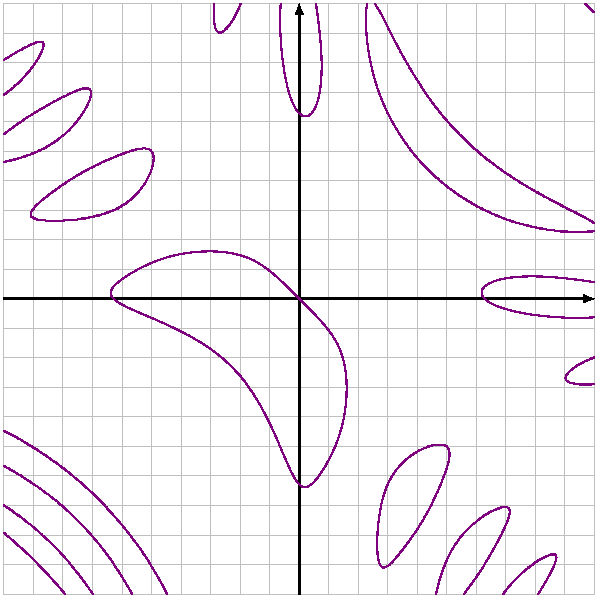
\includegraphics{tkz-grapheur-implicit-ex1.pdf}%
\hfill\null
\end{tcblisting}

\begin{tcblisting}{listing engine=minted,minted language=latex,colframe=lightgray,colback=lightgray!5,listing only}
\begin{GraphiqueTikz}%
    [x=1.5cm,y=1.5cm,Xmin=-2,Xmax=2,Ymin=-2,Ymax=2]
  \TracerAxesGrilles{}{}
  \TracerCourbeImplicite[Couleur=blue]{x*y^2+2*x^3*y^3-y-1}
\end{GraphiqueTikz}
\end{tcblisting}

\begin{tcblisting}{listing engine=minted,minted language=latex,colframe=lightgray,colback=lightgray!5,text only}
\hfill%
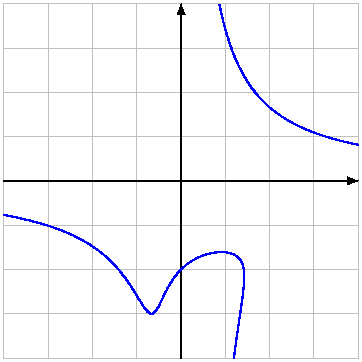
\includegraphics{tkz-grapheur-implicit-ex2.pdf}%
\hfill\null
\end{tcblisting}

\subsubsection{Courbes de niveaux}

En complément de la commande précédente, une commande de tracé de lignes de niveau est proposé, sous la forme $f(x,y)=k$, sur la même base.

À noter qu'une clé \MontreCode{[Couleurs=...]} a été rajoutée pour permettre de proposer une liste (qui sera traitée comme cyclique) de couleurs.

\begin{tcblisting}{listing engine=minted,minted language=latex,colframe=lightgray,colback=lightgray!5,listing only}
\TracerLignesNiveau[clés]{expression f(x,y)}{valeurs de k}
\end{tcblisting}

\begin{tcblisting}{listing engine=minted,minted language=latex,colframe=lightgray,colback=lightgray!5,listing only}
\begin{GraphiqueTikz}%
    [x=1.2cm,y=1.2cm,Xmin=-3,Xmax=3,Ymin=-3,Ymax=3]
  \TracerAxesGrilles{auto}{auto}
  % sin(x)*cos(y) = k  →  lignes de niveau d'une surface ondulée
  \TracerLignesNiveau%
    [Couleurs={blue!80,blue!50,cyan,teal,green!60!black}]%
    {sin(x)*cos(y)}%
    {-0.8,-0.6,-0.4,-0.2,0,0.2,0.4,0.6,0.8}
\end{GraphiqueTikz}
\end{tcblisting}

\begin{tcblisting}{listing engine=minted,minted language=latex,colframe=lightgray,colback=lightgray!5,text only}
\hfill%
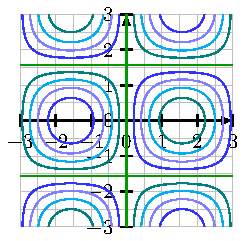
\includegraphics{tkz-grapheur-cbesniv.pdf}%
\hfill\null
\end{tcblisting}

\pagebreak

\subsection{Diagramme circulaire, diagramme annulaire}\label{diagcirculaire}\label{diagannulaire}

De manière expérimentale, il est possible de tracer un diagramme circulaire (camembert), dans un environnement \MontreCode{tikzpicture} standard (et non dans \MontreCode{GraphiqueTikz}).

\smallskip

{\footnotesize\faBomb}~Ces commandes sont expérimentales. La couleur de chaque secteur est \textbf{obligatoire} dans la liste de données.

\begin{tcblisting}{listing engine=minted,minted language=latex,colframe=lightgray,colback=lightgray!5,listing only}
%dans un environnement tikzpicture
\TracerDiagrammeCirculaire[clés]{liste}
\TracerDiagrammeAnneau[clés]{liste}
\LegendeCirculaire[clés]{liste}
\end{tcblisting}

La \MontreCode{liste} est spécifiée sous la forme \MontreCode{label/valeur/couleur/style,...}.

\smallskip

Les \MontreCode{[clés]} sont :

\begin{itemize}
  \item \MontreCode{Rayon=...} : rayon du cercle (en unités \TikZ), \MontreCode{3} par défaut ;
  \item \MontreCode{RayonInt=...} : rayon intérieur du cercle (en unités \TikZ), \MontreCode{1.75} par défaut ;
  \item \MontreCode{Titre=...} : titre affiché au-dessus du diagramme, vide par défaut.
\end{itemize}

\smallskip

Les \MontreCode{[clés]} de \MontreCode{\textbackslash LegendeCirculaire} sont :

\begin{itemize}
  \item \MontreCode{TailleCarreau=...} : taille des carreaux colorés, \MontreCode{0.28} par défaut ;
  \item \MontreCode{Espacement=...} : espacement vertical entre les entrées, \MontreCode{0.55} par défaut ;
  \item \MontreCode{DecalEst=...} : décalage horizontal depuis \MontreCode{cam-est}, \MontreCode{0.4} par défaut ;
  \item \MontreCode{Pct} : booléen, \MontreCode{true} par défaut, pour afficher les pourcentages (sinon les valeurs brutes) ;
  \item \MontreCode{Arrondi=...} : décimales pour l'affichage, \MontreCode{0} par défaut.
\end{itemize}

\smallskip

Après \MontreCode{\textbackslash DiagrammeCirculaire}, les nœuds suivants sont disponibles pour placer des éléments manuellement :

\begin{itemize}
  \item \MontreCode{cam-centre}, \MontreCode{cam-nord}, \MontreCode{cam-sud}, \MontreCode{cam-est}, \MontreCode{cam-ouest} : nœuds cardinaux ;
  \item \MontreCode{cam-i-debut}, \MontreCode{cam-i-fin} : points sur le cercle aux bornes du secteur $i$ ;
  \item \MontreCode{cam-i-mil} : point sur le cercle à l'angle médian du secteur $i$ ;
  \item \MontreCode{cam-i-int} : point intérieur (68\,\% du rayon), pour labels dans le secteur ;
  \item \MontreCode{cam-i-ext} : point extérieur (115\,\% du rayon), pour ligne et label externe.
\end{itemize}

\smallskip

\MontreCode{\textbackslash LegendeCirculaire} s'ancre automatiquement sur \MontreCode{cam-est}, elle doit donc être appelée après \MontreCode{\textbackslash DiagrammeCirculaire}, dans le même \MontreCode{tikzpicture}.

\begin{tcblisting}{listing engine=minted,minted language=latex,colframe=lightgray,colback=lightgray!5}
\def\DONNEES{%
  Français/24/cyan!60/solid,%
  Mathématiques/21/orange!70/north east lines,%
  Anglais/10/orange!40/crosshatch,%
  Arts plastiques/12/green!60/bricks,%
  Éducation physique/18/violet!80/vertical lines,%
  Musique/15/cyan!40/dots%
}

\begin{tikzpicture}[line join=bevel]
  \TracerDiagrammeCirculaire%
    [Titre={Répartition des matières}]{\DONNEES}
  \LegendeCirculaire{\DONNEES}
\end{tikzpicture}

\begin{tikzpicture}[line join=bevel]
  \TracerDiagrammeAnneau%
    [Rayon=2,RayonInt=1.25,Titre={Répartition des matières}]%
    {\DONNEES}
  \LegendeCirculaire{\DONNEES}
\end{tikzpicture}
\end{tcblisting}

\begin{tcblisting}{listing engine=minted,minted language=latex,colframe=lightgray,colback=lightgray!5}
\def\DONNEES{%
  Français/24/cyan!60/,%
  Mathématiques/21/orange!70/,%
  Anglais/10/orange!40/,%
  Arts plastiques/12/green!60/,%
  Éducation physique/18/violet!80/,%
  Musique/15/cyan!40/%
}

%effectifs bruts + labels manuels sur les grands secteurs
\begin{tikzpicture}[line join=bevel]
  \TracerDiagrammeCirculaire[]{\DONNEES}
  \LegendeCirculaire%
    [Pct=false,DecalEst=0.3]{\DONNEES}
  %labels manuels via les nœuds
  \node[align=center,font=\small] at (cam-1-int) {Français} ;
  \node[align=center,font=\small] at (cam-2-int) {Maths} ;
  \draw[gray,thin] (cam-3-mil) -- (cam-3-ext) ;
  \node[right,font=\small] at (cam-3-ext) {Anglais} ;
  %visualisation des nœuds créés (secteur 5)
  \filldraw[red] (cam-5-debut) circle[radius=2pt]
                 (cam-5-fin) circle[radius=2pt]
                 (cam-5-mil) circle[radius=2pt]
                 (cam-5-int) circle[radius=2pt]
                 (cam-5-ext) circle[radius=2pt] ;
\end{tikzpicture}
\end{tcblisting}

\pagebreak

\section{Commandes numériques}\label{outilnums}

\subsection{Introduction}

En marge des commandes graphiques, des commandes numériques ont été intégrées au package \MontreCode{tkz-grapheur}.

Les résultats obtenus sont \textit{bruts}, afin de pouvoir être réutilisés (arrondis, formatage) ultérieurement.

\smallskip

Les commandes présentées dans cette section sont des \textit{moteurs de calcul numérique} utilisables dans et hors de l'environnement \MontreCode{GraphiqueTikz}.

Elles stockent leurs résultats dans des macros et/ou les affichent directement. La convention est :

\begin{itemize}
  \item sans étoile \MontreCode{\textbackslash commande\{...\}} : affiche le résultat ;
  \item avec étoile \MontreCode{\textbackslash commande*\{...\}[\textbackslash macro]} : stocke le résultat dans \MontreCode{\textbackslash macro} (défaut : \MontreCode{\textbackslash mycalcres}).
\end{itemize}

\subsection{Analyse}

\subsubsection{Maximum, minimum}

\begin{tcblisting}{listing engine=minted,minted language=latex,colframe=lightgray,colback=lightgray!5,listing only}
\tkzgCalcMax[precision]{expr}{deb}{fin}[\macromax][\macroxmax]
\tkzgCalcMax[precision]{expr}{deb}{fin}[\macromin][\macroxmin]
\end{tcblisting}

\begin{itemize}
  \item \MontreCode{[précision]} : précision décimale.
\end{itemize}

\begin{tcblisting}{listing engine=minted,minted language=latex,colframe=lightgray,colback=lightgray!5}
\tkzgCalcMax{80*x*exp(-0.2*x)}{3}{10}\tmpmax\ en \tmpmaxvalx
\end{tcblisting}

\begin{tcblisting}{listing engine=minted,minted language=latex,colframe=lightgray,colback=lightgray!5}
\tkzgCalcMin[0.001]
  {log(exp(-x)+1)+0.25*x}{1}{1.2}
  [\MonMin]
  [\MonMinX]
\MonMin\ en \MonMinX
\end{tcblisting}

\subsubsection{Taux d'accroissement, nombre dérivée}

\begin{tcblisting}{listing engine=minted,minted language=latex,colframe=lightgray,colback=lightgray!5,listing only}
\tkzgTauxAccroiss*{expression}{a}{h}[\macro]

\tkzgDeriveeNum*[précision]<gd>{expr}{a}[\macro]
\end{tcblisting}

\begin{itemize}
  \item \MontreCode{[précision]} : précision décimale.
\end{itemize}

\begin{tcblisting}{listing engine=minted,minted language=latex,colframe=lightgray,colback=lightgray!5}
% entre 2 et 2 + 0.5, avec f(x)=x^2
\tkzgTauxAccroiss{x**2}{2}{0.5}
\end{tcblisting}

\begin{tcblisting}{listing engine=minted,minted language=latex,colframe=lightgray,colback=lightgray!5}
% en x=3 : f'(3) = 6
\tkzgDeriveeNum{x^2}{3}           % symétrique → 6.000...
\tkzgDeriveeNum<d>{x^2}{3}        % droite → 6.0001...
\tkzgDeriveeNum<g>{x^2}{3}        % gauche → 5.9999...

% en x=0 (borne gauche) : utiliser <d>
\tkzgDeriveeNum<d>{x^2}{0}        % → 0.0001...

% f(x) = sin(x), f'(0) = 1
\tkzgDeriveeNum{sin(x)}{0}        % → 1.000...
\end{tcblisting}

\subsubsection{Intégrale numérique (méthode de Simpson)}

\begin{tcblisting}{listing engine=minted,minted language=latex,colframe=lightgray,colback=lightgray!5,listing only}
\tkzgCalcIntegrale[N]{expression}{a}{b}
\tkzgCalcIntegrale*[N]{expression}{a}{b}[\macro]
\end{tcblisting}

\begin{itemize}
  \item \MontreCode{[N]} : nombre de subdivisions (\MontreCode{50} par défaut).
\end{itemize}

\begin{tcblisting}{listing engine=minted,minted language=latex,colframe=lightgray,colback=lightgray!5}
$\displaystyle\int_0^{\pi} \sin(x)\,\mathrm{d}x \approx \tkzgCalcIntegrale{sin(x)}{0}{pi}$

\tkzgCalcIntegrale*{sin(x)}{0}{pi}[\monres]
$\displaystyle\int_0^{\pi} \sin(x)\,\mathrm{d}x \approx \monres$
\end{tcblisting}

\subsubsection{Résolution approchée par dichotomie}

\begin{tcblisting}{listing engine=minted,minted language=latex,colframe=lightgray,colback=lightgray!5,listing only}
\tkzgResolApproch[precision]{equation}{a:b}
\tkzgResolApproch*[precision]{equation}{a:b}[\macro]

%avec vérification TVI (f(a)*f(b)<0)
\tkzgResolApprochTVI[precision]{equation}{a:b}
\tkzgResolApprochTVI*[precision]{equation}{a:b}[\macro]
\end{tcblisting}

\begin{itemize}
  \item \MontreCode{[precision]} : précision en valeur absolue (\MontreCode{0.001} par défaut) ;
  \item \MontreCode{\{equation\}} : équation de la forme \MontreCode{f(x)=valeur} ou simplement \MontreCode{f(x)} (résolution $=0$) ;
  \item \MontreCode{\{a:b\}} : intervalle de recherche.
\end{itemize}

La version \MontreCode{TVI} vérifie que $f(a) \times f(b)<0$ avant de lancer la dichotomie — si ce n'est pas le cas, la macro retourne \MontreCode{???}.

\begin{tcblisting}{listing engine=minted,minted language=latex,colframe=lightgray,colback=lightgray!5}
%résolution de e^x = 3 sur [0;2]
$x \approx \tkzgResolApproch{exp(x)=3}{0:2}$

%stockage
\tkzgResolApproch*{exp(x)=3}{0:2}[\monx]
$x \approx \monx$
\end{tcblisting}

\subsubsection{Seuil d'une suite récurrente}

\begin{tcblisting}{listing engine=minted,minted language=latex,colframe=lightgray,colback=lightgray!5,listing only}
\tkzgCalcSeuilSuite[Nmax]{f(x)}{n0}{u0}{signe}{seuil}
\tkzgCalcSeuilSuite*[Nmax]{f(x)}{n0}{u0}{signe}{seuil}[\macro]
\end{tcblisting}

\begin{itemize}
  \item \MontreCode{\{f(x)\}} : relation de récurrence $u_{n+1} = f(u_n)$ ;
  \item \MontreCode{\{n0\}}, \MontreCode{u0} : rang et valeur initiaux ;
  \item \MontreCode{\{signe\}} : condition d'arrêt parmi \MontreCode{>}, \MontreCode{<}, \MontreCode{>=}, \MontreCode{<=} ;
  \item \MontreCode{\{seuil\}} : valeur seuil à atteindre ;
  \item \MontreCode{[Nmax]} : nombre maximal d'itérations (\MontreCode{1000} par défaut) — sécurité anti-boucle infinie.
\end{itemize}

\begin{tcblisting}{listing engine=minted,minted language=latex,colframe=lightgray,colback=lightgray!5}
%premier n tel que 1.05^n > 2
\tkzgCalcSeuilSuite*{1.05*x}{0}{1}{>}{2}[\monrang]
$n_0 = \monrang$
\end{tcblisting}

\subsection{Probabilités}

\subsubsection{Lois discrètes}

\textbf{-- Loi binomiale}

\begin{tcblisting}{listing engine=minted,minted language=latex,colframe=lightgray,colback=lightgray!5,listing only}
%P(X=k)
\tkzgCalcBinomP{n}{p}{k}
\tkzgCalcBinomP*{n}{p}{k}[\macro]

%P(a<=X<=b)  (a/b = * => borne naturelle, 0 ou n)
\tkzgCalcBinomC{n}{p}{a}{b}
\tkzgCalcBinomC*{n}{p}{a}{b}[\macro]
\end{tcblisting}

\begin{tcblisting}{listing engine=minted,minted language=latex,colframe=lightgray,colback=lightgray!5}
% X -> B(10 ; 0.3)
$P(X=3) \approx \tkzgCalcBinomP{10}{0.3}{3}$

$P(X \leqslant 4) \approx \tkzgCalcBinomC{10}{0.3}{*}{4}$

$P(2 \leqslant X \leqslant 5) \approx \tkzgCalcBinomC{10}{0.3}{2}{5}$
\end{tcblisting}

\textbf{-- Loi de Poisson}

\begin{tcblisting}{listing engine=minted,minted language=latex,colframe=lightgray,colback=lightgray!5,listing only}
%P(X=k)
\tkzgCalcPoissP{lambda}{k}
\tkzgCalcPoissP*{lambda}{k}[\macro]

%P(a<=X<=b)
\tkzgCalcPoissC{lambda}{a}{b}
\tkzgCalcPoissC*{lambda}{a}{b}[\macro]
\end{tcblisting}

\begin{tcblisting}{listing engine=minted,minted language=latex,colframe=lightgray,colback=lightgray!5}
% Y -> P(5)
$P(Y=3) \approx \tkzgCalcPoissP{5}{3}$

$P(Y \geqslant 2) \approx \tkzgCalcPoissC{5}{2}{*}$
\end{tcblisting}

\textbf{-- Loi géométrique}

\begin{tcblisting}{listing engine=minted,minted language=latex,colframe=lightgray,colback=lightgray!5,listing only}
%P(X=k)
\tkzgCalcGeomP{p}{k}
\tkzgCalcGeomP*{p}{k}[\macro]

%P(a<=X<=b)
\tkzgCalcGeomC{p}{a}{b}
\tkzgCalcGeomC*{p}{a}{b}[\macro]
\end{tcblisting}

\begin{tcblisting}{listing engine=minted,minted language=latex,colframe=lightgray,colback=lightgray!5}
% T -> G(0.3)
$P(T=4) \approx \tkzgCalcGeomP{0.3}{4}$

$P(T \leqslant 5) \approx \tkzgCalcGeomC{0.3}{*}{5}$
\end{tcblisting}

\textbf{-- Loi hypergéométrique}

\begin{tcblisting}{listing engine=minted,minted language=latex,colframe=lightgray,colback=lightgray!5,listing only}
%P(X=k)   N=population  n=tirage  m=succès dans population

\tkzgCalcHypergeomP{N}{n}{m}{k}
\tkzgCalcHypergeomP*{N}{n}{m}{k}[\macro]

%P(a<=X<=b)
\tkzgCalcHypergeomC{N}{n}{m}{a}{b}
\tkzgCalcHypergeomC*{N}{n}{m}{a}{b}[\macro]
\end{tcblisting}

\begin{tcblisting}{listing engine=minted,minted language=latex,colframe=lightgray,colback=lightgray!5}
% W -> H(50,10,6)
$P(W=3) \approx \tkzgCalcHypergeomP{50}{6}{10}{3}$

$P(1 \leqslant W \leqslant 4) \approx \tkzgCalcHypergeomC{50}{6}{10}{1}{4}$
\end{tcblisting}

\subsubsection{Lois continues}

\textbf{-- Loi normale}

\begin{tcblisting}{listing engine=minted,minted language=latex,colframe=lightgray,colback=lightgray!5,listing only}
%P(a<=X<=b)  (a/b = * => borne infinie)
\tkzgCalcNormC{mu}{sigma}{a}{b}
\tkzgCalcNormC*{mu}{sigma}{a}{b}[\macro]
\end{tcblisting}

\begin{tcblisting}{listing engine=minted,minted language=latex,colframe=lightgray,colback=lightgray!5}
% X -> N(100 ; 10)
$P(X \leqslant 115) \approx \tkzgCalcNormC{100}{10}{*}{115}$

$P(90 \leqslant X \leqslant 110) \approx \tkzgCalcNormC{100}{10}{90}{110}$

$P(X \geqslant 120) \approx \tkzgCalcNormC{100}{10}{120}{*}$
\end{tcblisting}

\textbf{-- Loi exponentielle}

\begin{tcblisting}{listing engine=minted,minted language=latex,colframe=lightgray,colback=lightgray!5,listing only}
%P(a<=X<=b)  (a/b = * => 0 pour a, +inf approché pour b)
\tkzgCalcExpoC{lambda}{a}{b}
\tkzgCalcExpoC*{lambda}{a}{b}[\macro]
\end{tcblisting}

\begin{tcblisting}{listing engine=minted,minted language=latex,colframe=lightgray,colback=lightgray!5}
% Z -> Exp(0.1)
$P(Z \geqslant 5) \approx \tkzgCalcExpoC{0.1}{5}{*}$

$P(3 \leqslant Z \leqslant 8) \approx \tkzgCalcExpoC{0.1}{3}{8}$
\end{tcblisting}

\textbf{-- Loi de Student}

\begin{tcblisting}{listing engine=minted,minted language=latex,colframe=lightgray,colback=lightgray!5,listing only}
%P(a<=T_nu<=b)  [N] = subdivisions Simpson (50 par défaut)
\tkzgCalcStudentC[N]{nu}{a}{b}
\tkzgCalcStudentC*[N]{nu}{a}{b}[\macro]
\end{tcblisting}

\begin{tcblisting}{listing engine=minted,minted language=latex,colframe=lightgray,colback=lightgray!5}
% T -> Student(5)
$P(-2 \leqslant T \leqslant 2) \approx \tkzgCalcStudentC{5}{-2}{2}$

$P(T \geqslant 1.5) \approx \tkzgCalcStudentC{5}{1.5}{*}$
\end{tcblisting}

\textbf{-- Loi de Fischer}

\begin{tcblisting}{listing engine=minted,minted language=latex,colframe=lightgray,colback=lightgray!5,listing only}
%P(a<=F_{d1,d2}<=b)  attention : a > 0 !
\tkzgCalcFischerC[N]{d1}{d2}{a}{b}
\tkzgCalcFischerC*[N]{d1}{d2}{a}{b}[\macro]
\end{tcblisting}

\begin{tcblisting}{listing engine=minted,minted language=latex,colframe=lightgray,colback=lightgray!5}
% F -> Fischer(5,10)
$P(1 \leqslant F \leqslant 3) \approx \tkzgCalcFischerC{5}{10}{1}{3}$
\end{tcblisting}

\subsubsection{Quantiles}

\textbf{-- Loi normale}

\begin{tcblisting}{listing engine=minted,minted language=latex,colframe=lightgray,colback=lightgray!5,listing only}
%P(X<=k)=p
\tkzgQuantileNormal{mu}{sigma}{p}
\tkzgQuantileNormal*{mu}{sigma}{p}[\macro]

%P(X>k)=p
\tkzgQuantileNormalSup{mu}{sigma}{p}
\tkzgQuantileNormalSup*{mu}{sigma}{p}[\macro]

%P(mu-h<X<mu+h)=p  -> retourne h
\tkzgQuantileNormalCentre{mu}{sigma}{p}
\tkzgQuantileNormalCentre*{mu}{sigma}{p}[\macro]
\end{tcblisting}

\begin{tcblisting}{listing engine=minted,minted language=latex,colframe=lightgray,colback=lightgray!5}
% X -> N(100 ; 10)
$k$ tel que $P(X \leqslant k)=0{,}95$ :
$k \approx \tkzgQuantileNormal{100}{10}{0.95}$

$k$ tel que $P(X > k)=0{,}05$ :
$k \approx \tkzgQuantileNormalSup{100}{10}{0.05}$

$h$ tel que $P(100-h \leqslant X \leqslant 100+h)=0{,}95$ :
$h \approx \tkzgQuantileNormalCentre{100}{10}{0.95}$
\end{tcblisting}

\textbf{-- Loi binomiale}

\begin{tcblisting}{listing engine=minted,minted language=latex,colframe=lightgray,colback=lightgray!5,listing only}
%plus petit k tel que P(X<=k)>=p
\tkzgQuantileBinom{n}{p}{seuil}
\tkzgQuantileBinom*{n}{p}{seuil}[\macro]

%plus grand k tel que P(X>=k)>=p
\tkzgQuantileBinomSup{n}{p}{seuil}
\tkzgQuantileBinomSup*{n}{p}{seuil}[\macro]
\end{tcblisting}

\begin{tcblisting}{listing engine=minted,minted language=latex,colframe=lightgray,colback=lightgray!5}
% X -> B(20 ; 0.3)
plus petit $k$ tel que $P(X \leqslant k) \geqslant 0{,}95$ :
$k = \tkzgQuantileBinom{20}{0.3}{0.95}$

plus grand $k$ tel que $P(X \geqslant k) \geqslant 0{,}05$ :
$k = \tkzgQuantileBinomSup{20}{0.3}{0.05}$
\end{tcblisting}

\subsubsection{Intervalles de fluctuation et de confiance}

\begin{tcblisting}{listing engine=minted,minted language=latex,colframe=lightgray,colback=lightgray!5,listing only}
%intervalle de fluctuation : p=proportion théorique, n=taille échantillon
\tkzgCalcIntFluctu<seuil>[niveau]{p}{n}[\borneinf][\bornesup]
\tkzgCalcIntFluctu*<seuil>[niveau]{p}{n}[\borneinf][\bornesup]

%intervalle de confiance : f=fréquence observée, n=taille échantillon
\tkzgCalcIntConf<seuil>[niveau]{f}{n}[\borneinf][\bornesup]
\tkzgCalcIntConf*<seuil>[niveau]{f}{n}[\borneinf][\bornesup]
\end{tcblisting}

\begin{itemize}
  \item \MontreCode{<seuil>} : niveau de probabilité parmi \MontreCode{90}, \MontreCode{95} (défaut), \MontreCode{99}, ou \MontreCode{val} ;
  \item \MontreCode{[niveau]} : niveau scolaire parmi \MontreCode{2de} et \MontreCode{Term} ;
  \item \MontreCode{\textbackslash borneinf}, \MontreCode{\textbackslash bornesup} : macros de stockage des bornes (défaut : \MontreCode{\textbackslash myborneinf}, \MontreCode{\textbackslash mybornesup}).
\end{itemize}

\begin{tcblisting}{listing engine=minted,minted language=latex,colframe=lightgray,colback=lightgray!5}
%IF à 95% niveau Term, p=0.6, n=500
\tkzgCalcIntFluctu*{0.6}{500}[\myif][\myifs]
$I_f = [\myif;\myifs]$

%IC à 95% niveau Term, f=0.63, n=500
\tkzgCalcIntConf*{0.63}{500}[\myic][\myics]
$I_c = [\myic;\myics]$
\end{tcblisting}

\subsection{Statistiques}

\subsubsection{Paramètres statistiques}

\begin{tcblisting}{listing engine=minted,minted language=latex,colframe=lightgray,colback=lightgray!5,listing only}
%liste simple
\tkzgCalcParamStats{liste}[min][Q1][mediane][Q3][max]

%liste avec effectifs (valeur/effectif, séparateur .)
\tkzgCalcParamStats*{liste}[min][Q1][mediane][Q3][max]
\end{tcblisting}

Des résultats sont également stockés automatiquement dans :

\begin{itemize}
  \item \MontreCode{\textbackslash mamoyenne} : moyenne ;
  \item \MontreCode{\textbackslash monecarttype} : écart-type.
\end{itemize}

\begin{tcblisting}{listing engine=minted,minted language=latex,colframe=lightgray,colback=lightgray!5}
\tkzgCalcParamStats{2,5,3,8,4,7,6,1,9,5}
Min : \monmin, Q1 : \monquartileun, Médiane : \mamediane,
Q3 : \monquartiletrois, Max : \monmax,
Moyenne : \mamoyenne, Écart-type : \monecarttype
\end{tcblisting}

\subsubsection{Moyenne et écart-type}

\begin{tcblisting}{listing engine=minted,minted language=latex,colframe=lightgray,colback=lightgray!5,listing only}
%liste simple
\tkzgCalcMoyEctype{liste}[\moyenne][\ecarttype]

%liste avec effectifs
\tkzgCalcMoyEctype*{liste}[\moyenne][\ecarttype]
\end{tcblisting}

\begin{tcblisting}{listing engine=minted,minted language=latex,colframe=lightgray,colback=lightgray!5}
\tkzgCalcMoyEctype{2,5,3,8,4,7,6,1,9,5}[\mamoy][\monect]
Moyenne : \mamoy, Écart-type : \monect

%avec effectifs : valeur/effectif
\tkzgCalcMoyEctype*{10/3,20/5,30/2}[\mamoy][\monect]
Moyenne : \mamoy, Écart-type : \monect
\end{tcblisting}

\subsection{Sommes de termes de suites}

\subsubsection{Somme générale}

\begin{tcblisting}{listing engine=minted,minted language=latex,colframe=lightgray,colback=lightgray!5,listing only}
\tkzgCalcSommeSuite{expr(k)}{deb}{fin}
\tkzgCalcSommeSuite*{expr(k)}{deb}{fin}[\macro]
\end{tcblisting}

\begin{itemize}
  \item \MontreCode{\{expr(k)\}} : expression du terme général en fonction de \MontreCode{k} ;
  \item \MontreCode{\{deb\}}, \MontreCode{\{fin\}} : bornes inférieure et supérieure de la somme.
\end{itemize}

\begin{tcblisting}{listing engine=minted,minted language=latex,colframe=lightgray,colback=lightgray!5}
%somme des 10 premiers entiers
$\displaystyle\sum_{k=1}^{10} k = \tkzgCalcSommeSuite{k}{1}{10}$

%somme avec stockage
\tkzgCalcSommeSuite*{k^2}{1}{5}[\monres]
$\displaystyle\sum_{k=1}^{5} k^2 = \monres$
\end{tcblisting}

\subsubsection{Somme d'une suite arithmétique}

\begin{tcblisting}{listing engine=minted,minted language=latex,colframe=lightgray,colback=lightgray!5,listing only}
\tkzgCalcSommeArithm{p}{a}{r}{n}
\tkzgCalcSommeArithm*{p}{a}{r}{n}[\macro]
\end{tcblisting}

\begin{itemize}
  \item \MontreCode{\{p\}} : rang initial ;
  \item \MontreCode{\{a\}} : valeur initiale $u_p$ ;
  \item \MontreCode{\{r\}} : raison ;
  \item \MontreCode{\{n\}} : rang final.
\end{itemize}

\begin{tcblisting}{listing engine=minted,minted language=latex,colframe=lightgray,colback=lightgray!5}
%u0=3, raison=2, somme de u0 à u10
$S = \tkzgCalcSommeArithm{0}{3}{2}{10}$

\tkzgCalcSommeArithm*{0}{3}{2}{10}[\monres]
$S = \monres$
\end{tcblisting}

\subsubsection{Somme d'une suite géométrique}

\begin{tcblisting}{listing engine=minted,minted language=latex,colframe=lightgray,colback=lightgray!5,listing only}
\tkzgCalcSommeGeo{p}{a}{q}{n}
\tkzgCalcSommeGeo*{p}{a}{q}{n}[\macro]
\end{tcblisting}

\begin{itemize}
  \item \MontreCode{\{p\}} : rang initial ;
  \item \MontreCode{\{a\}} : valeur initiale $u_p$ ;
  \item \MontreCode{\{q\}} : raison ;
  \item \MontreCode{\{n\}} : rang final.
\end{itemize}

\begin{tcblisting}{listing engine=minted,minted language=latex,colframe=lightgray,colback=lightgray!5}
%u0=1, raison=0.5, somme de u0 à u8
$S = \tkzgCalcSommeGeo{0}{1}{0.5}{8}$

\tkzgCalcSommeGeo*{0}{1}{0.5}{8}[\monres]
$S = \monres$
\end{tcblisting}

\subsubsection{Somme d'une suite récurrente}

\begin{tcblisting}{listing engine=minted,minted language=latex,colframe=lightgray,colback=lightgray!5,listing only}
\tkzgCalcSommeSuiteRecurr{f(x)}{p}{up}{n}
\tkzgCalcSommeSuiteRecurr*{f(x)}{p}{up}{n}[\macro]
\end{tcblisting}

\begin{itemize}
  \item \MontreCode{\{f(x)\}} : relation de récurrence $u_{n+1}=f(u_n)$ ;
  \item \MontreCode{\{p\}}, \MontreCode{\{up\}} : rang et valeur initiaux ;
  \item \MontreCode{\{n\}} : rang final.
\end{itemize}

\begin{tcblisting}{listing engine=minted,minted language=latex,colframe=lightgray,colback=lightgray!5}
%u0=100, un+1=1.03*un, somme de u0 à u5
$S = \tkzgCalcSommeSuiteRecurr{1.03*x}{0}{100}{5}$

\tkzgCalcSommeSuiteRecurr*{1.03*x}{0}{100}{5}[\monres]
$S \approx \monres$
\end{tcblisting}

\subsection{Taux d'évolution}

\subsubsection{Taux d'évolution}

\begin{tcblisting}{listing engine=minted,minted language=latex,colframe=lightgray,colback=lightgray!5,listing only}
\tkzgCalcTauxEvol{VA}{VD}
\tkzgCalcTauxEvol*{VA}{VD}[\macro]
\end{tcblisting}

\begin{itemize}
  \item \MontreCode{\{VA\}} : valeur d'arrivée ;
  \item \MontreCode{\{VD\}} : valeur de départ.
\end{itemize}

Le résultat est le taux $t = \dfrac{V_A - V_D}{V_D}$, exprimé sous forme décimale.

\begin{tcblisting}{listing engine=minted,minted language=latex,colframe=lightgray,colback=lightgray!5}
%passage de 80 à 92
$t = \tkzgCalcTauxEvol{92}{80}$

\tkzgCalcTauxEvol*{92}{80}[\montaux]
$t \approx \num{\montaux}$
\end{tcblisting}

\subsubsection{Taux réciproque}

\begin{tcblisting}{listing engine=minted,minted language=latex,colframe=lightgray,colback=lightgray!5,listing only}
\tkzgCalcTauxReciproque{t}
\tkzgCalcTauxReciproque*{t}[\macro]
\end{tcblisting}

\begin{itemize}
  \item \MontreCode{\{t\}} : taux d'évolution (sous forme décimale).
\end{itemize}

Le résultat est le taux réciproque $t' = \dfrac{1}{1+t} - 1$.

\begin{tcblisting}{listing engine=minted,minted language=latex,colframe=lightgray,colback=lightgray!5}
%taux réciproque d'une augmentation de 15%
$t' = \tkzgCalcTauxReciproque{0.15}$

\tkzgCalcTauxReciproque*{0.15}[\treciproque]
$t' \approx \num{\treciproque}$
\end{tcblisting}

\subsubsection{Taux moyen}

\begin{tcblisting}{listing engine=minted,minted language=latex,colframe=lightgray,colback=lightgray!5,listing only}
\tkzgCalcTauxMoyen{t}{n}
\tkzgCalcTauxMoyen*{t}{n}[\macro]
\end{tcblisting}

\begin{itemize}
  \item \MontreCode{\{t\}} : taux global d'évolution (sous forme décimale) ;
  \item \MontreCode{\{n\}} : nombre de périodes.
\end{itemize}

Le résultat est le taux moyen $t_m = (1+t)^{1/n} - 1$.

\begin{tcblisting}{listing engine=minted,minted language=latex,colframe=lightgray,colback=lightgray!5}
%taux moyen d'une augmentation globale de 30% sur 5 ans
$t_m = \tkzgCalcTauxMoyen{0.30}{5}$

\tkzgCalcTauxMoyen*{0.30}{5}[\tmoy]
$t_m \approx \num{\tmoy}$
\end{tcblisting}

\pagebreak

\section{Codes source des exemples de la page d'accueil}

\begin{tcblisting}{listing engine=minted,minted language=latex,colframe=lightgray,colback=lightgray!5}
\begin{GraphiqueTikz}[x=0.85cm,y=0.35cm,Xmin=0,Xmax=10,Ymin=0,Ymax=16]
  %préparation de la fenêtre
  \TracerAxesGrilles[Derriere,Elargir=2.5mm,Police=\small]{0,1,...,10}{0,2,...,16}
  %déf des fonctions avec nom courbe + nom fonction + expression (tracés à la fin !)
  \DefinirCourbe[Nom=cf]<f>{3*x-6}
  \DefinirCourbe[Nom=cg]<g>{-(x-6)^2+12}
  %antécédents et intersection
  \TrouverIntersections[Aff=false,Nom=K]{cf}{cg}
  \TrouverAntecedents[AffDroite,Couleur=orange,Nom=I]{cg}{8}
  \TrouverAntecedents[Aff=false,Nom=J]{cg}{0}
  %intégrale sous une courbe, avec intersection
  \TracerIntegrale%
    [Couleurs=blue/purple,Bornes=noeuds,Style=hachures,Hachures=bricks]%
    {g(x)}%
    {(I-2)}{(J-2)}
  %intégrale entre les deux courbes
  \TracerIntegrale[Bornes=noeuds,Type=fct/fct]%
    {f(x)}[g(x)]%
    {(K-1)}{(K-2)}
  %tracé des courbes et des points
  \TracerCourbe[Couleur=red]{f(x)}
  \TracerCourbe[Couleur=teal]{g(x)}
  \PlacerPoints<\small>{(K-1)/below right/L,(K-2)/above left/M}%
  \PlacerPoints[violet]<\small>{(I-1)/above left/D,(I-2)/above right/E}%
  %tangente
  \TracerTangente[Couleurs=pink!75!black/yellow,kl=2,kr=2,AffPoint]{g}{5}
  %images
  \PlacerImages[Couleurs=cyan]{g}{7,7.25,7.5}
  %surimpression des axes
  \TracerAxesGrilles[Devant,Elargir=2.5mm]{0,1,...,10}{0,2,...,16}
\end{GraphiqueTikz}
\end{tcblisting}

\pagebreak

\begin{tcblisting}{listing engine=minted,minted language=latex,colframe=lightgray,colback=lightgray!5}
\begin{GraphiqueTikz}%
  [x=3.5cm,y=4cm,
  Xmin=0,Xmax=3.5,Xgrille=pi/12,Xgrilles=pi/24,
  Ymin=-1.05,Ymax=1.05,Ygrille=0.2,Ygrilles=0.05]
  %préparation de la fenêtre
  \TracerAxesGrilles[Derriere,Elargir=2.5mm,Format=ntrig/nsqrt]{}{}
  %rajouter des valeurs
  \RajouterValeursAxeX{0.25,1.4,3.3}{\num{0.25},\num{1.4},\num{3.3}}
  %fonction trigo (déf + tracé)
  \DefinirCourbe[Nom=ccos,Debut=0,Fin=pi]<fcos>{cos(x)}
  \DefinirCourbe[Nom=csin,Debut=0,Fin=pi]<fsin>{sin(x)}
  %intégrale
  \TrouverIntersections[Aff=false,Nom=JKL]{ccos}{csin}
  \TracerIntegrale%
    [Bornes=noeud/abs,Type=fct/fct,Couleurs=cyan/cyan!50]%
    {fsin(x)}[fcos(x)]%
    {(JKL-1)}{pi}
  %tracé des courbes
  \TracerCourbe[Couleur=red,Debut=0,Fin=pi]{fcos(x)}
  \TracerCourbe[Couleur=olive,Debut=0,Fin=pi]{fsin(x)}
  %antécédent(s)
  \PlacerAntecedents[Couleurs=blue/teal!50!black,Traits]{ccos}{-0.25}
  \PlacerAntecedents[Couleurs=red/magenta!50!black,Traits]{csin}{0.5}
  \PlacerAntecedents[Couleurs=orange/orange!50!black,Traits]{csin}{sqrt(2)/2}
  \PlacerAntecedents[Couleurs=green!50!black/green,Traits]{csin}{sqrt(3)/2}
  %surimpression axes
  \TracerAxesGrilles[Devant,Format=ntrig/nsqrt]%
    {pi/6,pi/4,pi/3,pi/2,2*pi/3,3*pi/4,5*pi/6,pi}
    {0,sqrt(2)/2,1/2,sqrt(3)/2,1,-1,-sqrt(3)/2,-1/2,-sqrt(2)/2}
\end{GraphiqueTikz}
\end{tcblisting}

\newpage

\section{Commandes auxiliaires}

\subsection{Intro}

En marge des commandes purement \textit{graphiques}, quelques commandes auxiliaires sont disponibles :

\begin{itemize}
  \item une pour formater un nombre avec une précision donnée ;
  \item une pour travailler sur des nombres aléatoires, avec contraintes.
\end{itemize}

\subsection{Arrondi formaté}\label{numarrond}

La commande \MontreCode{\textbackslash ArrondirNum} permet de formater, grâce au package \MontreCode{siunitx}, un nombre (ou un calcul), avec une précision donnée. Cela peut être \textit{utile} pour formater des résultats obtenus grâce aux commandes de récupération des coordonnées, par exemple.

\begin{tcblisting}{listing engine=minted,minted language=latex,colframe=lightgray,colback=lightgray!5,listing only}
\ArrondirNum[précision]{calcul xint}
\end{tcblisting}

\begin{tcblisting}{listing engine=minted,minted language=latex,colframe=lightgray,colback=lightgray!5}
\ArrondirNum{1/3}\\
\ArrondirNum{16.1}\\
\ArrondirNum[3]{log(10)}\\
\end{tcblisting}

\subsection{Gestion de listes}\label{gestlistes}

Les commandes suivantes permettent de travailler sur les listes \textsf{CSV} générées automatiquement via la clé \MontreCode{ListeRes} ou manuellement via
\MontreCode{\textbackslash CreerListeAbscisses}.

\begin{description}
  \item[\textbackslash\texttt{CreerListeAbscisses\{préfixe\}\{nb\}\{nom\}}]
  Construit une liste CSV des abscisses des nœuds \textsf{préfixe-1},
  \textsf{préfixe-2}, \ldots, \textsf{préfixe-nb}, et la stocke dans la macro \verb|\nom|. Si \MontreCode{nb} vaut \MontreCode{0}, la macro est laissée vide sans erreur.
  \item[\textbackslash\texttt{tkzgCalcLongueurListe{*}\{liste\}{[macro]}}]
  Retourne le nombre d'éléments de la liste CSV \MontreCode{liste}.
  La version étoilée stocke le résultat dans \MontreCode{macro} sans
  l'afficher~; la version normale affiche également le résultat.
  \item[\textbackslash\texttt{tkzgCalcElementListe{*}\{liste\}\{index\}{[macro]}}]
  Retourne l'élément d'index \MontreCode{index} de la liste CSV
  \MontreCode{liste}. L'index peut être positif (depuis le début) ou négatif
  (depuis la fin)~: \MontreCode{-1} désigne ainsi le dernier élément.
  La version étoilée stocke sans afficher.
\end{description}

Ces trois commandes s'articulent naturellement avec les itérateurs de
\textsf{xint}, notamment \MontreCode{\textbackslash xintFor*} et
\MontreCode{\textbackslash xintNthElt}, pour parcourir ou exploiter les
listes générées.

\pagebreak

\subsection{Nombre aléatoire sous contraintes}\label{nbalea}

L'idée de cette deuxième commande est de pouvoir déterminer un nombre aléatoire :

\begin{itemize}
  \item entier ou décimal ;
  \item sous contraintes (entre deux valeurs fixées).
\end{itemize}

Cela peut permettre, par exemple, de travailler sur des courbes avec points \textit{aléatoires}, mais respectant certaines contraintes.

\begin{tcblisting}{listing engine=minted,minted language=latex,colframe=lightgray,colback=lightgray!5,listing only}
\ChoisirNbAlea(*)[precision (déf 0)]{borne inf}{borne sup}[\macro]
\end{tcblisting}

La version étoilée prend les contraintes sous forme stricte ($\text{borne inf} < \text{macro} < \text{borne sup}$) alors que la version normale prend les contraintes sous forme large ($\text{borne inf} \leqslant \text{macro} \leqslant \text{borne sup}$).

\smallskip

À noter que les \textit{bornes} peuvent être des \textit{macros} existantes !

\begin{tcblisting}{listing engine=minted,minted language=latex,colframe=lightgray,colback=lightgray!5}
%un nombre (2 chiffres après la virgule) entre 0.75 et 0.95
%un nombre (2 chiffres après la virgule) entre 0.05 et 0.25
%un nombre (2 chiffres après la virgule) entre 0.55 et \YrandMax
%un nombre (2 chiffres après la virgule) entre \YrandMin et 0.45
\ChoisirNbAlea[2]{0.75}{0.95}[\YrandMax]%
\ChoisirNbAlea[2]{0.05}{0.25}[\YrandMin]%
\ChoisirNbAlea*[2]{0.55}{\YrandMax}[\YrandA]%
\ChoisirNbAlea*[2]{\YrandMin}{0.45}[\YrandB]%
%vérification
\num{\YrandMax} \& \num{\YrandMin} \& \num{\YrandA} \& \num{\YrandB}
\end{tcblisting}

\begin{tcblisting}{listing engine=minted,minted language=latex,colframe=lightgray,colback=lightgray!5}
%un nombre (2 chiffres après la virgule) entre 0.75 et 0.95
%un nombre (2 chiffres après la virgule) entre 0.05 et 0.25
%un nombre (2 chiffres après la virgule) entre 0.55 et \YrandMax
%un nombre (2 chiffres après la virgule) entre \YrandMin et 0.45
\ChoisirNbAlea[2]{0.75}{0.95}[\YrandMax]%
\ChoisirNbAlea[2]{0.05}{0.25}[\YrandMin]%
\ChoisirNbAlea*[2]{0.55}{\YrandMax}[\YrandA]%
\ChoisirNbAlea*[2]{\YrandMin}{0.45}[\YrandB]%
%vérification
\num{\YrandMax} \& \num{\YrandMin} \& \num{\YrandA} \& \num{\YrandB}
\end{tcblisting}

\begin{tcblisting}{listing engine=minted,minted language=latex,colframe=lightgray,colback=lightgray!5}
%la courbe est prévue pour qu'il y ait 3 antécédents
\ChoisirNbAlea[2]{0.75}{0.95}[\YrandMax]%
\ChoisirNbAlea[2]{0.05}{0.25}[\YrandMin]%
\ChoisirNbAlea*[2]{0.55}{\YrandMax}[\YrandA]%
\ChoisirNbAlea*[2]{\YrandMin}{0.45}[\YrandB]%

\begin{GraphiqueTikz}
  [x=0.075cm,y=7.5cm,Xmin=0,Xmax=150,Xgrille=10,Xgrilles=5,
  Ymin=0,Ymax=1,Ygrille=0.1,Ygrilles=0.05]
  \TracerAxesGrilles[Dernier,Elargir=2.5mm]{auto}{auto}
  \DefinirCourbeInterpo[Couleur=red,Trace,Nom=fonctiontest,Tension=0.75]
  {(0,\YrandA)(40,\YrandMin)(90,\YrandMax)(140,\YrandB)}
  \TrouverAntecedents[Aff=false,Nom=ANTECED]{fonctiontest}{0.5}
  \PlacerAntecedents[Couleurs=blue/teal,Traits]{fonctiontest}{0.5}
  \RecupererAbscisse{(ANTECED-1)}[\Aalpha]
  \RecupererAbscisse{(ANTECED-2)}[\Bbeta]
  \RecupererAbscisse{(ANTECED-3)}[\Cgamma]
\end{GraphiqueTikz}

Les solutions de $f(x)=\num{0.5}$ sont, par lecture graphique :
$\begin{cases}
  \alpha \approx \ArrondirNum[0]{\Aalpha} \\
  \beta \approx \ArrondirNum[0]{\Bbeta} \\
  \gamma \approx \ArrondirNum[0]{\Cgamma}
\end{cases}$.
\end{tcblisting}

\newpage

\subsection{Tableaux de valeurs}\label{tabval}

Les commandes suivantes permettent de générer un tableau de valeurs
pour une fonction \textsf{xint}, avec un choix de présentation
horizontale ou verticale.

\begin{itemize}
  \item \MontreCode{\textbackslash CalcTableauValeurs} génère uniquement
  le \textit{corps} du tableau, stocké dans une macro — l'utilisateur
  gère ensuite la mise en forme avec son environnement préféré
  (\MontreCode{tblr}, \MontreCode{NiceTabular}, \MontreCode{tabular}...) ;
  \item \MontreCode{\textbackslash ConstruireTableauValeurs} fait tout
  en un avec \MontreCode{tabularray} (nécessite de ce fait
  \MontreCode{\textbackslash usepackage\{tabularray\}} !).
\end{itemize}

\subsubsection{Génération du corps}

\begin{tcblisting}{listing engine=minted,minted language=latex,colframe=lightgray,colback=lightgray!5,listing only}
%horizontal (défaut)
\CalcTableauValeurs[clés]<nom/expr>{valeurs}{nomMacro}

%vertical (version étoilée)
\CalcTableauValeurs*[clés]<nom/expr>{valeurs}{nomMacro}
\end{tcblisting}

\begin{itemize}
  \item \MontreCode{<nom/expr>} : nom de fonction \textsf{xint}
  (défaut) ou expression directe si \MontreCode{Expr=true} ;
  \item \MontreCode{\{valeurs\}} : liste des valeurs de \MontreCode{x}
  (syntaxe \MontreCode{\textbackslash foreach} :
  \MontreCode{\{-2,-1,0,1,2\}} ou \MontreCode{\{-2,-1,...,2\}}) ;
  \item \MontreCode{\{nomMacro\}} : nom de la macro de sortie
  (sans \textbackslash) — crée \MontreCode{\textbackslash nomMacro}
  (le body) et \MontreCode{\textbackslash nomMacronbvals}
  (le nombre de colonnes/lignes) ;
  \item \MontreCode{Arrondi} : précision de l'arrondi
  (\MontreCode{2} par défaut) ;
  \item \MontreCode{NomFct} : label de la fonction dans le tableau
  (\MontreCode{f} par défaut) ;
  \item \MontreCode{NomVar} : label de la variable dans le tableau
  (\MontreCode{x} par défaut) ;
  \item \MontreCode{Expr} : booléen (\MontreCode{false} par défaut)
  — si \MontreCode{true}, \MontreCode{<...>} est une expression
  directe avec \MontreCode{x} comme variable.
\end{itemize}

\begin{tcblisting}{listing engine=minted,minted language=latex,colframe=lightgray,colback=lightgray!5}
%usepackage{tabularray}
\GenererFonction<f>{x^2+1}

%horizontal
\CalcTableauValeurs[Arrondi=1]<f>{-2,-1,0,1,2}[montab]

\begin{tblr}%
  [expand=\montab]%
  {%
    colspec={*{\montabnbvals}{c}},hlines,%
    row{1}={bg=gray!25,font=\bfseries}%
  }
  \montab
\end{tblr}
\end{tcblisting}

\begin{tcblisting}{listing engine=minted,minted language=latex,colframe=lightgray,colback=lightgray!5}
%vertical + expression directe
\CalcTableauValeurs*%
  [Expr,NomFct=g,NomVar=t]%
  <x^2+1>{0,1,2,3}[montabv]

\begin{tblr}%
  [expand=\montabv]%
  {%
    colspec={*{2}{c}},hlines,%
    row{1}={bg=blue!15,font=\bfseries}%
  }
  \montabv
\end{tblr}
\end{tcblisting}

\subsubsection{Tableau complet avec \textsf{tabularray}}

\begin{tcolorbox}[colframe=orange,colback=orange!5]
Cette commande nécessite le chargement préalable de
\MontreCode{tabularray} — un avertissement est émis sinon.
\end{tcolorbox}

\begin{tcblisting}{listing engine=minted,minted language=latex,colframe=lightgray,colback=lightgray!5,listing only}
%horizontal (défaut, Presentation=H)
\ConstruireTableauValeurs[clés]<options tblr>{nom/expr}{valeurs}

%vertical (Presentation=V)
\ConstruireTableauValeurs[clés,Presentation=V]<options tblr>{nom/expr}{valeurs}
\end{tcblisting}

\begin{itemize}
  \item \MontreCode{[clés]} : mêmes clés que
  \MontreCode{\textbackslash CalcTableauValeurs} ;
  \item \MontreCode{<options tblr>} : options passées directement à l'environnement ;
  \item \MontreCode{Presentation} : \MontreCode{H} (horizontal, défaut) ou \MontreCode{V} (vertical) ;
  \item \MontreCode{\textbackslash tdvnbvals} : macro exposée contenant le nombre de colonnes — utile pour \MontreCode{colspec}.
\end{itemize}

\begin{tcblisting}{listing engine=minted,minted language=latex,colframe=lightgray,colback=lightgray!5}
\GenererFonction<f>{x^2+1}

%horizontal
\ConstruireTableauValeurs%
  [Arrondi=2]%
  <colspec={*{\tdvnbvals}{c}},hlines,row{1}={bg=gray!25,font=\bfseries}>%
  {f}{-2,-1,0,1,2}

%vertical
\ConstruireTableauValeurs%
  [Arrondi=2,Presentation=V]%
  <colspec={*{2}{c}},hlines,row{1}={bg=gray!25,font=\bfseries}>%
  {f}{0,0.5,...,2}
\end{tcblisting}

\newpage

\section{Liste des commandes}

\NewDocumentCommand\lstcmd{ m m m }{%
  \item[\footnotesize\texttt{#1}]{\footnotesize : \hyperref[#3]{\mintinline{latex}|#2|}\hfill{}page \pageref{#3}}
}

\subsection{Environnement, axes et grilles}

\begin{description}[noitemsep]
  \lstcmd{environnement~~}{\begin{GraphiqueTikz}...\end{GraphiqueTikz}}{creaenvt}
  \lstcmd{axes et grilles}{\TracerAxesGrille}{creaaxesgr}
  \lstcmd{ax/gril pol~~~~}{\TracerAxesGrillePol}{courbespolaires}
  \lstcmd{aj val axes X~~}{\RajouterValeursAxeX}{ajoutvals}
  \lstcmd{aj val axes Y~~}{\RajouterValeursAxeY}{ajoutvals}
  \lstcmd{semilog loglog~}{}{loglog}
\end{description}

\subsection{Courbes, suites}

\begin{description}[noitemsep]
  \lstcmd{def formule~~~~}{\GenererFonction}{genererfct}
  \lstcmd{def fonction~~~}{\DefinirCourbe}{deftracfct}
  \lstcmd{tracé courbe~~~}{\TracerCourbe}{deftracfct}
  \lstcmd{def interpo~~~~}{\DefinirCourbeInterpo}{deftracinterpo}
  \lstcmd{tracé interpo~~}{\TracerCourbeInterpo}{deftracinterpo}
  \lstcmd{interp Lagrange}{\GenererPolynomeLagrange}{lagrangeinterpo}
  \lstcmd{def Taylor~~~~~}{\DefinirTaylor}{taylor}
  \lstcmd{tracé Taylor~~~}{\TracerTaylor}{taylor}
  \lstcmd{def spline~~~~~}{\DefinirCourbeSpline}{deftracfctspline}
  \lstcmd{tracé spline~~~}{\TracerCourbeSpline}{deftracfctspline}
  \lstcmd{tracé droite~~~}{\TracerDroite}{tracdroite}
  \lstcmd{asymptote vert~}{\TracerAsymptote}{tracdroite}
  \lstcmd{tangente~~~~~~~}{\TracerTangente}{tgte}
  \lstcmd{nuage suite~~~~}{\TracerNuageSuite}{nuagesuite}
  \lstcmd{toile récurr~~~}{\TracerToileRecurrence}{toilerecurr}
  \lstcmd{déf fam cbes~~~}{\DefinirFamilleCourbes}{famcourbes}
  \lstcmd{trace famille~~}{\TracerFamilleCourbes}{famcourbes}
\end{description}

\subsection{Outils graphiques}

\begin{description}[noitemsep]
  \lstcmd{def points~~~~~}{\DefinirPts}{defpts}
  \lstcmd{def image~~~~~~}{\DefinirImage}{defpts}
  \lstcmd{marq pts~~~~~~~}{\MarquerPts}{markpts}
  \lstcmd{placer txt~~~~~}{\PlacerTexte}{placetxt}
  \lstcmd{pts discont~~~~}{\AfficherPtsDiscont}{ptsdiscont}
  \lstcmd{récup absc~~~~~}{\RecupererAbscisse}{recupcoordo}
  \lstcmd{récup ordo~~~~~}{\RecupererOrdonnee}{recupcoordo}
  \lstcmd{récup coordos~~}{\RecupererCoordonnees}{recupcoordo}
  \lstcmd{images~~~~~~~~~}{\PlacerImages}{images}
  \lstcmd{antécédents~~~~}{\TrouverAntecedents}{defanteced}
  \lstcmd{antécédents~~~~}{\PlacerAntecedents}{tracanteced}
  \lstcmd{intersection~~~}{\TrouverIntersections}{intersect}
  \lstcmd{maximum~~~~~~~~}{\TrouverMaximum}{maximum}
  \lstcmd{minimum~~~~~~~~}{\TrouverMinimum}{minimum}
  \lstcmd{dérivée~~~~~~~~}{\TracerDerivee}{derivprimit}
  \lstcmd{inég. linéaire~}{\InegaliteLineaire}{ineglin}
  \lstcmd{primitive~~~~~~}{\TracerPrimitive}{derivprimit}
  \lstcmd{transform refl~}{\TracerReflexion}{transformfreflex}
  \lstcmd{transform~~~~~~}{\TracerTransformee}{transform}
\end{description}

\subsection{Intégrales, probabilités, statistiques}

\begin{description}[noitemsep]
  \lstcmd{intégrale~~~~~~}{\TracerIntegrale}{integr}
  \lstcmd{méthodes int~~~}{\RepresenterMethodeIntegrale}{methodesintergrales}
  \lstcmd{Monte-Carlo~~~~}{\SimulerMonteCarlo}{montecarlo}
  \lstcmd{loi normale~~~~}{\DefinirLoiNormale}{loinormale}
  \lstcmd{loi normale~~~~}{\TracerLoiNormale}{loinormale}
  \lstcmd{loi expo~~~~~~~}{\DefinirLoiExpo}{loiexpo}
  \lstcmd{loi expo~~~~~~~}{\TracerLoiExpo}{loiexpo}
  \lstcmd{loi khideux~~~~}{\DefinirLoiKhiDeux}{loikhideux}
  \lstcmd{loi khideux~~~~}{\TracerLoiKhiDeux}{loikhideux}
  \lstcmd{loi binom~~~~~~}{\TracerHistoBinomiale}{histobinom}
  \lstcmd{loi Poisson~~~~}{\TracerLoiPoisson}{loipoisson}
  \lstcmd{loi géom~~~~~~~}{\TracerLoiGeo}{loigeo}
  \lstcmd{loi hypergéo~~~}{\TracerLoiHyperGeo}{loihypergeo}
  \lstcmd{loi Student~~~~}{\DefinirLoiStudent}{loistudent}
  \lstcmd{loi Student~~~~}{\TracerLoiStudent}{loistudent}
  \lstcmd{loi Fischer~~~~}{\DefinirLoiFischer}{loifischer}
  \lstcmd{loi Fischer~~~~}{\TracerLoiFischer}{loifischer}
  \lstcmd{aire continue~~}{\RepresenterProbaContinue}{loiinteg}
  \lstcmd{courbe ECC~~~~~}{\TracerCourbeECC}{cbeECC}
  \lstcmd{stats 2 var~~~~}{\TracerNuage}{nuage}
  \lstcmd{regressions~~~~}{\TracerAjustement}{regressions}
  \lstcmd{nuage transfo~~}{\TracerNuagePoints}{nuagetransfo}
  \lstcmd{diagramme~~~~~~}{\TracerDiagrammeBatons}{diagbatons}
  \lstcmd{histogramme~~~~}{\TracerHistogramme}{histogramme}
  \lstcmd{moustaches~~~~~}{\TracerBoiteMoustaches}{boitemoustaches}
\end{description}

\subsection{Courbes polaires, paramétriques}

\begin{description}[noitemsep]
  \lstcmd{déf param~~~~~~}{\DefinirCourbeParam}{courbesparam}
  \lstcmd{trac param~~~~~}{\TracerCourbeParam}{courbesparam}
  \lstcmd{déf param~~~~~~}{\DefinirCourbeParam}{courbesparam}
  \lstcmd{trac param~~~~~}{\TracerCourbeParam}{courbesparam}
  \lstcmd{déf polaire~~~~}{\DefinirCourbePol}{courbespolaires}
  \lstcmd{trac polaire~~~}{\TracerCourbePol}{courbespolaires}
\end{description}

\subsection{Coniques}

\begin{description}[noitemsep]
  \lstcmd{ellipse~~~~~~~~}{\TracerEllipse}{coniques}
  \lstcmd{ellipse param~~}{\AfficherElementsEllipse}{coniques}
  \lstcmd{parabole~~~~~~~}{\TracerParabole}{coniques}
  \lstcmd{parabol param~~}{\AfficherElementsParabole}{coniques}
  \lstcmd{hyperbole~~~~~~}{\TracerHyperbole}{coniques}
  \lstcmd{hyperbol param~}{\AfficherElementsHyperbole}{coniques}
\end{description}

\subsection{Commandes diverses}

\begin{description}[noitemsep]
  \lstcmd{vals interd~~~~}{ValeursInterdites=...}{valinterdites}
  \lstcmd{voisinages~~~~~}{\AfficherVoisinage}{voisinages}
  \lstcmd{diag camembert~}{\TracerDiagrammeCirculaire}{diagcirculaire}
  \lstcmd{diaganneau~~~~~}{\TracerDiagrammeAnneau}{diagannulaire}
  \lstcmd{arrondi~~~~~~~~}{\ArrondirNum}{numarrond}
  \lstcmd{nb aléat~~~~~~~}{\ChoisirNbAlea}{nbalea}
  \lstcmd{gestion listes~}{}{gestlistes}
  \lstcmd{outils num~~~~~}{}{outilnums}
  \lstcmd{tab valeurs~~~~}{\ConstruireTableauValeurs}{tabval}
  \lstcmd{gestion csv~~~~}{\CreerListesDepuisCSV}{csv}
  \lstcmd{cbe implicite~~}{\TracerCourbeImplicite}{implicit}
\end{description}

\newpage

\section{Quelques commandes liées à pgfplots}

\subsection{Introduction}

Pour des graphiques avec des fenêtres d'affichage \textit{particulières}, il est fort possible que les commandes \textit{classiques} de \MontreCode{tkz-grapheur} coincent, avec notamment des \MontreCode{dimension too large}$\ldots$

\smallskip

Dans ce cas, il est possible d'utiliser plutôt l'environnement \MontreCode{axis} de \MontreCode{pgfplots}, qui, de plus, permet \textit{souvent} de pallier ce problème \textit{interne}$\ldots$

\MontreCode{tkz-grapheur} ne fournit pas d'environnement dédié pour la création de la fenêtre, mais quelques commandes spécifiques ont été intégrées pour certains points, avec un fonctionnement assez semblable (donc se référer aux paragraphes précédents) à celui des commandes \textit{classiques}.

\subsection{Macros spécifique pgfplots/axis}

\begin{tcblisting}{listing engine=minted,minted language=latex,colframe=lightgray,colback=lightgray!5,listing only}
%déterminer l'intersection de deux objets préalablement définis via [name path]
\findintersectionspgf[base nom nœuds]{objet1}{objet2}[macro nb total]

%extraction (globale, non limitée à l'environnement) et stockage de coordonnées
\gextractxnodepgf{nœud}[\myxcoord]
\gextractynodepgf{nœud}[\myycoord]
\gextractxynodepgf{nœud}[\myxcoord][\myycoord]

%domaine entre courbes
\fillbetweencurvespgf[options tikz]{courbe1}{courbe2}<options soft domain>

%splines cubiques
\addplotspline(*)[options tikz]<coeffs>{liste des points support}[\monspline]
\end{tcblisting}

\subsection{Exemple illustré}

\begin{tcblisting}{listing only,listing engine=minted,minted language=latex,colframe=lightgray,colback=lightgray!5}
%\usepackage{alphalph}

\begin{tikzpicture}
  \begin{axis}%
    [%
    axis y line=center,axis x line=middle,                                   %axes
    axis line style={line width=0.8pt,-latex},
    x=0.33cm,y=0.55cm,xmin=1985,xmax=2030,ymin=56,ymax=70,                   %unités
    grid=both,xtick distance=5,ytick distance=2,                             %grillep
    minor x tick num=4,minor y tick num=1,                                   %grilles
    extra x ticks={1985},extra x tick style={grid=none},                     %origx
    extra y ticks={56},extra y tick style={grid=none},                       %origy
    x tick label style={/pgf/number format/.cd,use comma,1000 sep={}},       %année
    major tick length={2*3pt},minor tick length={1.5*3pt},                   %grads
    every tick/.style={line width=0.8pt},enlargelimits=false,                %style
    enlarge x limits={abs=2.5mm,upper},enlarge y limits={abs=2.5mm,upper},   %élargir
    ]
    %spline + y=66
    \addplot[name path global=eqtest,mark=none,red,line width=1.05pt,domain=1985:2030] {66} ;
    \def\LISTETEST{1985/60/0§1995/68/0§2015/58/0§2025/69/0§2030/62/-2}
    \addplotspline*[line width=1.05pt,violet,name path global=splinecubtest]{\LISTETEST}[\monsplineviolet]
    %recherche d'antécédents
    \findintersectionspgf[MonItsc]{eqtest}{splinecubtest}
    %extraction des coordonnées
    \gextractxnodepgf{(MonItsc-1)}[\xMonItscA]
    \gextractxnodepgf{(MonItsc-2)}[\xMonItscB]
    \gextractxnodepgf{(MonItsc-3)}[\xMonItscC]
    \gextractxnodepgf{(MonItsc-4)}[\xMonItscD]
    %visualisation
    \xintFor* #1 in {\xintSeq{1}{4}}\do{%
      \draw[line width=0.9pt,densely dashed,olive,->,>=latex] (MonItsc-#1) -- (\csname xMonItsc\AlphAlph{#1}\endcsname,56) ;
      \filldraw[olive] (MonItsc-#1) circle[radius=1.75pt] ;
    }
    %intégrale
    \path [name path=xaxis] (1985,56) -- (2030,56);
    \fillbetweencurvespgf{splinecubtest}{xaxis}<domain={\xMonItscB:\xMonItscA}>
    \fillbetweencurvespgf{splinecubtest}{xaxis}<domain={\xMonItscD:\xMonItscC}>
  \end{axis}
\end{tikzpicture}

Les solutions de $f(x)=66$ sont d'environ \ArrondirNum*[0]{\xMonItscA} \&\ \ArrondirNum*[0]{\xMonItscB} \&\ \ArrondirNum*[0]{\xMonItscC} \&\ \ArrondirNum*[0]{\xMonItscD}.
\end{tcblisting}

\begin{tikzpicture}
  \begin{axis}%
    [%
    axis y line=center,axis x line=middle,                                   %axes
    axis line style={line width=0.8pt,-latex},
    x=0.33cm,y=0.55cm,xmin=1985,xmax=2030,ymin=56,ymax=70,                   %unités
    grid=both,xtick distance=5,ytick distance=2,                             %grillep
    minor x tick num=4,minor y tick num=1,                                   %grilles
    extra x ticks={1985},extra x tick style={grid=none},                     %originex
    extra y ticks={56},extra y tick style={grid=none},                       %originey
    x tick label style={/pgf/number format/.cd,use comma,1000 sep={}},       %année
    major tick length={2*3pt},minor tick length={1.5*3pt},                   %grads
    every tick/.style={line width=0.8pt},enlargelimits=false,                %style
    enlarge x limits={abs=2.5mm,upper},enlarge y limits={abs=2.5mm,upper},   %élargir
    ]
    %spline + y=66
    \addplot[name path global=eqtest,mark=none,red,line width=1.05pt,domain=1985:2030] {66} ;
    \def\LISTETEST{1985/60/0§1995/68/0§2015/58/0§2025/69/0§2030/62/-2}
    \addplotspline*[line width=1.05pt,violet,name path global=splinecubtest]{\LISTETEST}[\monsplineviolet]
    %recherche d'antécédents
    \findintersectionspgf[MonItsc]{eqtest}{splinecubtest}
    %extraction des coordonnées
    \gextractxnodepgf{(MonItsc-1)}[\xMonItscA]
    \gextractxnodepgf{(MonItsc-2)}[\xMonItscB]
    \gextractxnodepgf{(MonItsc-3)}[\xMonItscC]
    \gextractxnodepgf{(MonItsc-4)}[\xMonItscD]
    %visualisation
    \xintFor* #1 in {\xintSeq{1}{4}}\do{%
      \draw[line width=0.9pt,densely dashed,olive,->,>=latex] (MonItsc-#1) -- (\csname xMonItsc\AlphAlph{#1}\endcsname,56) ;
      \filldraw[olive] (MonItsc-#1) circle[radius=1.75pt] ;
    }
    %intégrale
    \path [name path=xaxis] (1985,56) -- (2030,56);
    \fillbetweencurvespgf{splinecubtest}{xaxis}<domain={\xMonItscB:\xMonItscA}>
    \fillbetweencurvespgf{splinecubtest}{xaxis}<domain={\xMonItscD:\xMonItscC}>
  \end{axis}
\end{tikzpicture}

Les solutions de $f(x)=66$ sont d'environ \ArrondirNum*[0]{\xMonItscA} \&\ \ArrondirNum*[0]{\xMonItscB} \&\ \ArrondirNum*[0]{\xMonItscC} \&\ \ArrondirNum*[0]{\xMonItscD}.

\pagebreak

\section{Historique}

{\footnotesize \begin{quote}
\begin{verbatim}
0.30f : Ajouts en statistiques (barres/bâtons/histogrammes/moustaches/camembert)
0.30e : Meilleure gestion de la taille du graphique
-----   Améliorations dans les valeurs interdites
-----   Courbe de niveaux (expérimental)
0.30d : Ajout d'une clé pour créer une liste d'abscisse + exploitation de listes
-----   Famille de courbes (expérimental)
-----   Définition globales de fonctions (hors environnement ou via clé [DefGlobale])
-----   Tableau de valeurs (expérimental)
-----   Graphiques semi-log ou log-log (expérimental)
-----   Nuage de points avec transformations et/ou par csv (expérimental)
-----   Macros de calculs pour des évolutions en %, des sommes de suites
-----   Courbe implicite (très expérimental, lua)
0.30c : Refonte du fonctionnement avec séparation commandes [en/fr]
-----   Transformations, Taylor (expérimental)
-----   Ajout de lois de probabilités (continues + discrètes)
-----   Outils numériques
0.30b : Dérivée/primitive (expérimental)
-----   Nuage suites
-----   Courbes paramétrées, polaires
-----   Voisinages (expérimental)
-----   Valeurs interdites (expérimental)
-----   Coniques (expérimental)
0.30a : Création des nœuds (fenêtre + axes)
0.2.9 : Ajout de thèmes de couleurs pour les grilles
0.2.7 : Possibilité de spécifier les dimensions du graphique (en test)
0.2.6 : Inegalité linéaire (en test)
0.2.5 : Interpolation de Lagrange + améliorations
0.2.4 : Clé [StyleTrace] pour des pointillés par exemple
0.2.3 : Bugfix avec une longueur
0.2.0 : Méthode alternative des splines cubiques + commandes auxiliaires pgfplots
0.1.9 : Correction d'un bug avec la détermination d'unités
0.1.8 : Courbes ECC/FCC + Toile récurrence + Points discontinuité + HistoBinom
0.1.7 : Méthodes intégrales avec des splines
0.1.6 : Asymptote verticale + Méthodes intégrales (géom + Monte Carlo)
0.1.5 : Correction d'un bug sur les rajouts de valeurs + Nœud pour une image + [en] version !
0.1.4 : Placement de texte
0.1.3 : Ajout de régressions avec le package xint-regression
0.1.2 : Droites + Extremums
0.1.1 : Densité loi normale et khi deux + Marquage points + Améliorations
0.1.0 : Version initiale
\end{verbatim}
\end{quote}}

\end{document}